\documentclass[11pt]{article}
\usepackage{graphicx, color}
\usepackage[a4paper,margin=2cm]{geometry}

% \addtolength{\hoffset}{-2.25cm}
% \addtolength{\textwidth}{4.5cm}
% \addtolength{\voffset}{-3.25cm}
% \addtolength{\textheight}{5cm}
% \setlength{\parindent}{0in}

%----------------------------------------------------------------------------------------
%	PACKAGES AND OTHER DOCUMENT CONFIGURATIONS
%----------------------------------------------------------------------------------------
\usepackage[labelfont=bf]{caption}
\usepackage[]{subcaption}
\usepackage{multirow}
\usepackage[dvipsnames]{xcolor}
\definecolor{darkblue}{rgb}{0, 0, 0.5}
\usepackage{blindtext} % Package to generate dummy text
\usepackage{charter} % Use the Charter font
\usepackage[utf8]{inputenc} % Use UTF-8 encoding
\usepackage{microtype} % Slightly tweak font spacing for aesthetics
\usepackage[english]{babel} % Language hyphenation and typographical rules
\usepackage{amsthm, amsmath, amssymb, amsfonts, bbm, stmaryrd} % Mathematical typesetting
\usepackage{float} % Improved interface for floating objects
\usepackage[final, colorlinks=true, linkcolor=black, citecolor=darkblue, urlcolor=darkblue]{hyperref} % For hyperlinks in the PDF
\usepackage{graphicx, multicol} % Enhanced support for graphics
\usepackage{pgfplots} \pgfplotsset{compat=1.13}
\usepackage{xcolor} % Driver-independent color extensions
\usepackage{marvosym, wasysym} % More symbols
\usepackage{rotating} % Rotation tools
\usepackage{booktabs} % Enhances quality of tables
%\usepackage[numbers,sort]{natbib}
\usepackage[sort]{natbib}
\renewcommand\cite{\citep}
\usepackage{bm}
\usepackage{wrapfig}
\usepackage{enumitem}
\usepackage{csquotes} % Context sensitive quotation facilities
\usepackage[nodayofweek]{datetime} % Uses YEAR-MONTH-DAY format for dates
\usepackage{acronym}
\usepackage{adjustbox}
\usepackage{pifont}
\newcommand{\cmark}{\ding{51}}%
\newcommand{\xmark}{\ding{55}}%
\usepackage{nicefrac}
\let\rfb\reflectbox
\newcommand{\flipfracout}[2]{\rfb{\nicefrac{\rfb{#1}}{\rfb{#2}}}}
\newcommand{\flipfrac}[2]{\flipfracout{\ensuremath{#1}}{\ensuremath{#2}}}

\usepackage{fancyhdr} % Headers and footers
\pagestyle{fancy} % All pages have headers and footers
\fancyhead{}\renewcommand{\headrulewidth}{0pt} % Blank out the default header
\fancyfoot[L]{} % Custom footer text
\fancyfoot[C]{} % Custom footer text
\fancyfoot[R]{\thepage} % Custom footer text
% \newcommand{\note}[1]{\marginpar{\scriptsize \textcolor{red}{#1}}} % Enables comments in red on margin
\newcommand{\TODO}[1]{\textbf{\textcolor{red}{#1}}}
\newcommand{\note}[1]{\textit{\textcolor{blue}{Note: #1}}}
\newcommand{\rephrase}[1]{\textcolor{orange}{#1}}
\newcommand{\Comment}[1]{\textcolor{blue}{\textit{#1}}}
\newcommand{\E}[0]{\mathbb{E}}
\newcommand{\R}[0]{\mathbb{R}}

%----------------------------------------------------------------------------------------

\usepackage{fancyhdr}
% Headers
\usepackage{titlesec}
\titleformat{\section}[hang]
{\LARGE\bfseries}
{Section \thesection.}{0.4em}{}
\titlespacing{\section}{0pc}{0.5cm plus 0cm minus 0cm}{1cm plus .3cm minus .5cm}
\titleformat{\subsection}[hang]
{\fontsize{13pt}{12pt}\selectfont\bfseries}
{\thesubsection.}{0.4em}{}
\titlespacing{\subsection}{0pc}{0.5cm}{0.3cm}
\titlespacing{\paragraph}{%
  0pt}{%              left margin
  0.6\baselineskip}{% space before (vertical)
  0.75em}%               space after (horizontal)
\titleformat{\paragraph}[runin]
{\fontsize{10pt}{12pt}\selectfont\bfseries}
{\theparagraph}{0.4em}{}

% Figures
\captionsetup{aboveskip=0.2cm,belowskip=0.2cm}


% Acronyms 
\acrodef{NF}{normalizing flow}
\acrodef{VAE}{variational auto-encoder}
\acrodef{GAN}{generative adversarial network}
\acrodef{MC}{monte-carlo}
\acrodef{IWVAE}{importance-weighted VAE}
\acrodef{LDJ}{log-determinant Jacobian}
\acrodef{SOTA}{state-of-the-art}
\acrodef{CDF}{cumulative distribution function}
\acrodef{VI}{variational inference}
\acrodef{GNN}{graph neural network}
\acrodef{ELBO}{evidence lower bound}

\makeatletter
\renewenvironment{abstract}{%
    \if@twocolumn
      \section*{\abstractname}%
    \else %% <- here I've removed \small
      \begin{center}%
        {\bfseries \large\abstractname\vspace{\z@}}%  %% <- here I've added \large
      \end{center}%
      \quotation
    \fi}
    {\if@twocolumn\else\endquotation\fi}
\makeatother

\newcommand{\red}[1]{{\color{red}{#1}}}
\DeclareCaptionFont{xipt}{\fontsize{10}{12}\mdseries}

\begin{document}

\begin{titlepage} 

\newcommand{\HRule}{\rule{\linewidth}{0.5mm}} % Defines a new command for the horizontal lines, change thickness here
\center % Center everything on the page
 
%----------------------------------------------------------------------------------------
%	HEADING SECTIONS
%----------------------------------------------------------------------------------------


\includegraphics[width=0.8\linewidth]{figures/uvaENG.jpg}\\[2.5cm]
\textsc{\Large MSc Artificial Intelligence}\\[0.2cm]
% \textsc{\normalsize Track: \red{track}}\\[1.0cm] % track
\textsc{\Large Master Thesis}\\[0.5cm] 

%----------------------------------------------------------------------------------------
%	TITLE SECTION
%----------------------------------------------------------------------------------------

\HRule \\[0.4cm]
{ \huge \bfseries Categorical Normalizing Flows\\ via Continuous Transformations}\\[0.4cm] % Title of your document
\HRule \\[0.5cm]
 
%----------------------------------------------------------------------------------------
%	AUTHOR SECTION
%----------------------------------------------------------------------------------------

by\\[0.2cm]
\textsc{\Large Phillip Lippe}\\[0.2cm] %you name
12182451\\[1cm]


%----------------------------------------------------------------------------------------
%	DATE SECTION
%----------------------------------------------------------------------------------------

{\Large \today}\\[1cm] % Date, change the \today to a set date if you want to be precise

48 ECTS\\ %
November 2019 - July 2020\\[1cm]%

%----------------------------------------------------------------------------------------
%	COMMITTEE SECTION
%----------------------------------------------------------------------------------------
\begin{minipage}[t]{0.4\textwidth}
\begin{flushleft} \large
\emph{Supervisor:} \\
Dr. Efstratios Gavves\\
% Dr Jakub Tomczak % Supervisor's Name
\end{flushleft}
\end{minipage}
~
\begin{minipage}[t]{0.4\textwidth}
\begin{flushright} \large
\emph{Assessor:} \\
Dr. Max Welling\\
\end{flushright}
\end{minipage}\\[2cm]

%----------------------------------------------------------------------------------------
%	LOGO SECTION
%----------------------------------------------------------------------------------------

% \framebox{\rule{0pt}{2.5cm}\rule{2.5cm}{0pt}}\\[0.5cm]

\includegraphics[width=2.5cm]{figures/uvaLogo.pdf}\\[0.5cm] % Include a department/university logo - this will require the graphicx package
\textsc{\large Informatics Institute (IvI)\\Intelligent Sensory Information Systems (ISIS)}\\[1.0cm] % 
 
%----------------------------------------------------------------------------------------

\vfill % Fill the rest of the page with whitespace

\end{titlepage}

\fontsize{10.0}{12.0}\selectfont
\captionsetup{font=xipt}
\AtBeginEnvironment{tabular}{\fontsize{10.0}{12.0}\selectfont}
\AtBeginEnvironment{tabular*}{\fontsize{10.0}{12.0}\selectfont}

\pagenumbering{gobble}
\newpage
\text{ }
\newgeometry{top=3cm,bottom=3cm,left=2.75cm,right=2.75cm,headheight=17pt}
\pagenumbering{roman}
\pagestyle{fancy}
\fancyhf{}
\cfoot{\thepage}
\chead{\textit{\rightmark}}
\renewcommand{\headrulewidth}{0.5pt}
\renewcommand{\footrulewidth}{0.5pt}
\fancyheadoffset{0pt}

\newpage
\setcounter{tocdepth}{2}
\tableofcontents
\newpage
\listoffigures
\newpage
\listoftables
\newpage
\setlength{\parindent}{0pt}
\setlength{\parskip}{5.5pt}
\markboth{Abstract}{ABSTRACT}
\null\vspace{2cm}
\begin{abstract}
Despite their popularity, to date, the application of normalizing flows on categorical data stays limited.
The current practice of using dequantization to map discrete data to a continuous space is inapplicable as categorical data has no intrinsic order.
Instead, categorical data have complex and latent relations that must be inferred, like the synonymy between words. 
In this thesis, we
investigate \emph{Categorical Normalizing Flows}, that is normalizing flows for categorical data.
By casting the encoding of categorical data in continuous space as a variational inference problem, we jointly optimize the continuous representation and the model likelihood.
To maintain unique decoding, we learn a partitioning of the latent space by factorizing the posterior. 
Meanwhile, the complex relations between the categorical variables are learned by the ensuing normalizing flow, thus maintaining a close-to exact likelihood estimate and making it possible to scale up to a large number of categories.
Based on Categorical Normalizing Flows, we propose GraphCNF a permutation-invariant generative model on graphs, outperforming both one-shot and autoregressive flow-based state-of-the-art on molecule generation.\\

%\noindent Paper: \href{https://arxiv.org/abs/2006.09790}{https://arxiv.org/abs/2006.09790}\\ 
%Code: \href{https://github.com/phlippe/CategoricalNF}{https://github.com/phlippe/CategoricalNF}
    
\end{abstract}
\newpage
\pagenumbering{arabic}

\vspace*{0cm}
\section{Introduction}
\label{sec:introduction}

Generative deep learning models have gained increasing interest in recent years due to their many applications and real-world use cases \cite{Goodfellow2014GenerativeNets, StyleGAN, BigGAN, VAE, VQVAE2, NVAE}. 
Given a dataset, their goal is to model a distribution that describes the processes of generating the data.
One family of generative models which allows both efficient sampling (i.e. generating new data) and exact density evaluation (i.e. determining the likelihood of a sample) is normalizing flows \cite{NormalizingFlowsFundamentals, NormalizingFlowsOriginalMathConcept}. 
Normalizing flows model distributions by applying a sequence of invertible transformations mapping the input distribution to a known base distribution such as a factorized Gaussian. 
In contrast to other common generative models like \acp{GAN} and \acp{VAE}, normalizing flows do not suffer from training issues like mode collapse or posterior collapse \cite{VAEPosteriorCollapse, StyleGAN, NormalizingFlowsOverview}. 
Successful applications of normalizing flows include image generation \cite{RealNVP, Glow, Flow++, IntegerNF}, audio generation \cite{FloWaveNet, Waveglow} and reinforcement learning \cite{NFReinforcementLearning1, NFReinforcementLearning2}.

The recent advances of normalizing flows concentrated on continuous distributions because the concept normalizing flows rely on is the rule of change of variables, a continuous transformation naturally working on continuous data.
However, many real-world applications involve discrete data, such as natural language, graphs and sets (see Figure~\ref{fig:introduction_categorical_applications}). 
Naturally, applying continuous flows on these discrete data points would lead to an undesired, degenerate solution where all probability mass is placed on only these discrete values, making the modeled distribution useless \cite{UriaContPeaks, Theis2015}. 
For the application on images, where close-by values are strongly related (i.e. a pixel value of 127 and 128 are almost visually indistinguishable), a common solution is to add a small amount of noise to each value for dequantization \cite{RealNVP, Flow++}.
Such dequantization techniques, however, cannot be as simply applied on nominal discrete data where the values represent categories with no intrinsic order. 
Treating these categories as integers for dequantization
biases the data to a non-existing order, and makes the modeling task significantly harder. 
Previous insights on learning the noise distribution in dequantization, called variational dequantization \cite{Flow++, EmielDequantization}, have underlined the great importance of a flexible representation of ordinal data in normalizing flows, and hence we suspect a similar impact for categorical data.

\begin{figure}[b!]
    \centering
    \begin{subfigure}{.3\textwidth}
        \centering
        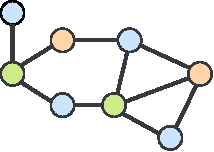
\includegraphics[height=2.5cm]{figures/intro_figures/graph_coloring.pdf}
        \caption{Combinatorial problems}
        \label{fig:introduction_applications_combinatorial_problems}
    \end{subfigure}
    \hfill
    \begin{subfigure}{.3\textwidth}
        \centering
        \vfill
        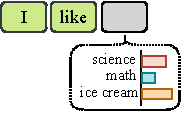
\includegraphics[height=2.5cm]{figures/intro_figures/language_modeling.pdf}
        \caption{Language modeling}
        \label{fig:introduction_applications_language_modeling}
    \end{subfigure}
    \hfill
    \begin{subfigure}{.3\textwidth}
        \centering
        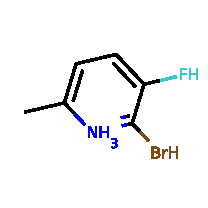
\includegraphics[height=2.5cm]{figures/intro_figures/zinc250k_tiny_981.pdf} %molecule_generation_rdkit.pdf}
        \caption{Molecule generation}
        \label{fig:introduction_applications_molecule_generation}
    \end{subfigure}
    \caption[Common applications and areas involving categorical distributions]{
    Common applications that involve categorical distributions include (a) combinatorial problems such as graph coloring, (b) language modeling and (c) use cases in biology and chemistry such as molecule generation. We will visit all three applications in experiments throughout this work.}
    \label{fig:introduction_categorical_applications}
\end{figure}

%%%%%%%%%%%%%%%%%%
%% Discrete NFs %%
%%%%%%%%%%%%%%%%%%
An alternative, which recently gained interested, is to apply normalizing flows directly on discrete distributions instead of continuous. 
This means that the input and the output distribution, as well as the intermediate steps in the flow model rely on discrete values. 
To implement this in a neural network, \citet{IntegerNF} proposed to use rounding operations on top of the continuous outputs of a neural flow to discretize it to the nearest integer. 
Another approach suggested by \citet{TranDiscreteFlows} operates on categorical distributions being suitable for non-ordinal data. 

However, while both have proven to work reasonably well in certain settings, there are considerable drawbacks with working directly on discrete space.
Firstly, discrete operations such as rounding or argmax are not differentiable, and thus cannot be used for backpropagation during training. 
Although solutions such as the straight-through estimator \cite{STEGradientEstimator} can approximate gradients for these operations, an experiment by \citet{IntegerNF} showed that a deep discrete flow obtains lower performance compared to a shallow flow.
This is because the gradient approximation accumulates bias with increasing depth, and destabilizes gradient-based optimization techniques \cite{IntegerNF, IDF++}.
Secondly, \citet{TranDiscreteFlows} discusses that their gradient approximation prevents them from scaling up to distributions with more than 200 categories.
Thus, such flows cannot be applied to large distributions like word-level language modeling.
Finally, discrete normalizing flows can only learn a permutation of its original input space, as the invertibility of the flow requires a one-to-one mapping from the input to the output \cite{SemiDiscreteNFSequence, IDF++, NormalizingFlowsOverview2}.
This limits the possible distributions it can model since with a uniform base distribution, any possible mapping learned by the flow will result in a uniform distribution.
Hence, discrete normalizing flows have to rely on powerful base distribution like autoregressive models as used in \cite{IntegerNF, TranDiscreteFlows}.

\begin{figure}[b!]
    \centering
    \begin{subfigure}{.48\textwidth}
        \centering
        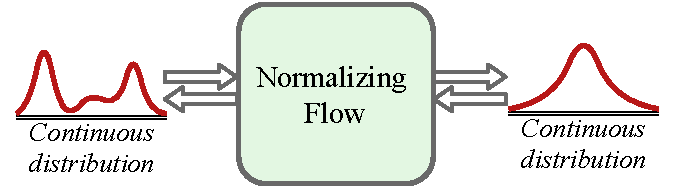
\includegraphics[width=\linewidth]{figures/intro_figures/GeneralNFs_Continuous_to_Continuous.pdf}
        \caption{Continuous Normalizing Flow}
        \label{fig:introduction_NFs_continuous_to_continuous}
    \end{subfigure}
    \hfill
    \begin{subfigure}{.48\textwidth}
        \centering
        
\includegraphics[width=\linewidth]{figures/intro_figures/GeneralNFs_Discrete_to_Discrete.pdf}
        \caption{Discrete Normalizing Flow}
        \label{fig:introduction_NFs_discrete_to_discrete}
    \end{subfigure}
    \begin{subfigure}{.48\textwidth}
        \centering
        
\includegraphics[width=\linewidth]{figures/intro_figures/GeneralNFs_Discrete_to_Continuous.pdf}
        \caption{Categorical Normalizing Flow}
        \label{fig:introduction_NFs_discrete_to_continuous}
    \end{subfigure}
    \caption[Comparison of Continuous, Discrete and Categorical Normalizing Flows]{
    Continuous normalizing flows are used to model a mapping between a complex, unknown continuous distribution to a base distribution like a Gaussian. 
    Discrete NFs map a discrete distribution to another by permuting its elements, being less flexible than a continuous flow.
    Our proposed approach, Categorical NF, also models discrete distributions, but stays with a continuous base distribution on the other side. This allows the usage of powerful continuous flows while operating on categorical data.}
    \label{fig:introduction_NFs_concept_semi_discrete}
\end{figure}

Meanwhile, continuous flows can learn much richer mappings between distributions. 
This allows them to model complex distributions using simple, factorized base distributions from which it can be efficiently sampled in parallel. 
Moreover, it has been theoretically shown that a flow on continuous data with sufficiently complex transformations can model a mapping between any two distributions \cite{NormalizingFlowsOriginalMathConcept, NormalizingFlowsOverview2}. 
Considering the issues of discrete normalizing flows, the question arises whether we can develop a method to apply powerful continuous flows on discrete, categorical input data.
Hence, in this work, we propose and investigate the framework of \emph{Categorical Normalizing Flows} which learn a mapping from a categorical distribution to a continuous base distribution while preserving a close-to exact likelihood estimate (see Figure~\ref{fig:introduction_NFs_discrete_to_continuous}). 




\subsection{Contributions}
\label{sec:introduction_contributions}

The first step in Categorical Normalizing Flows is to embed the discrete values into continuous space. 
Instead of pre-specifying non-overlapping volumes for each discrete value as done in dequantization, we propose to use variational inference as a toolkit to jointly optimize the mapping to continuous latent space and modeling the likelihood by a normalizing flow.
Previous work on combining variational inference with normalizing flows have mainly focused on improving the approximate posterior's flexibility \cite{InverseAutoregressiveFlows, NormalizingFlowsFundamentals, SylvesterNF}. 
Here, instead, we use variational inference to provide a continuous representation of the discrete data to a normalizing flow. 
Learning the continuous representation is crucial for categorical data as in contrast to integers, categories do not have an intrinsic order. On the contrary, there usually exist (hidden) relations between categories that may be beneficial to represent (i.e. similarity of word senses), and thus can be learned in Categorical Normalizing Flows.

To maintain a close-to exact likelihood estimate despite the introduced lower bound of the variational inference framework, the modeling of the categorical distribution needs to happen solely in the normalizing flow.
Thus, no information should be lost when mapping the data into continuous space.
We achieve this by limiting the encoding distributions to ones whose (approximate) posterior is independent over discrete variables. 
As a result, we obtain a learned partitioning of the latent space with an almost unique decoding, which is jointly learned with the model likelihood in continuous space.
We call this approach \emph{Categorical Normalizing Flows} and experiment with three different encoding distributions of increasing flexibility: (1) a mixture model where every category is represented by a logistic, (2) a model with additional flows applied to each category independently, and (3) a normalizing flow spanning across all variables, similar to variational dequantization.
Nonetheless, we find that in general a simple mixture model is sufficient for encoding categorical data well, and that increasing the complexity of the encoding distribution does not lead to a noticeable performance gain.

Categorical Normalizing Flows can be applied to any task involving categorical variables.
Examples, which we visit experimentally in this work, include words as categorical (one-hot vector) variables, sets and graphs~\cite{GraphOverview1, GraphOverview2}.
We put particular emphasis on graphs, as
current approaches are mostly autoregressive \cite{GraphRNNDeep, GraphAF, GraphRNN} and view graphs as sequences, although there exists no intrinsic order of the nodes. 
Normalizing flows, however, can perform generation in parallel making a definition of order unnecessary. 
By treating both nodes and edges as categorical variables, we employ our variational inference encoding and propose GraphCNF.
GraphCNF is a novel permutation-invariant normalizing flow on graph generation which assigns equal likelihood to any ordering of nodes. 
Meanwhile, GraphCNF encodes the node attributes, edge attributes and graph structure in three consecutive steps for efficiency.
As shown in the experiments on graph coloring and molecule generation, the improved encoding and flow architecture allows GraphCNF to outperform significantly both the autoregressive and parallel flow-based state-of-the-art.

Overall, our contributions are summarized as follows:
\begin{itemize}
	\item We propose Categorical Normalizing Flows, which apply a novel encoding method for categorical data in normalizing flows. 
	By using variational inference with a factorized posterior, we still support a close-to exact likelihood estimate and scale up to large number of categories.
	\item Building on the framework of Categorical Normalizing Flows, we propose GraphCNF, a permutation-invariant normalizing flow on graph generation.
	On molecule generation, GraphCNF sets a new state-of-the-art for flow-based methods, outperforming one-shot and autoregressive baselines. 
	\item We experiment with encoding distributions of increasing flexibility on various tasks including sets, language and graphs, and show that a simple mixture model is sufficient for modeling discrete, categorical distribution accurately. Moreover, we show that the encoding dimensionality also corresponds to the task's complexity underlining the importance of applying flexible, continuous flows on categorical data.
\end{itemize}


\subsection{Outline}
\label{sec:introduction_outline}
This thesis consists of six further sections. In Section~\ref{sec:background}, we review the fundamentals and common design choices of normalizing flows. 
The related work, including Discrete Normalizing Flows and combinations of \acp{VAE} and normalizing flows, is discussed in Section~\ref{sec:related_work}. 
Continuing in Section~\ref{sec:methodology}, we introduce the framework of Categorical Normalizing Flows in detail. Furthermore, we present GraphCNF, a permutation-invariant normalizing flow on graphs. 
Section~\ref{sec:experiments} discusses experiments on set modeling, graph coloring, molecule generation and language modeling that have been performed to evaluate and analyze the frameworks mentioned before. 
Finally, Section~\ref{sec:conclusion} concludes this thesis with a reflection of the results and suggestions for future work. 
\newpage
\section{Preliminaries}
\label{sec:background}

The following chapter provides an introduction to the field of Normalizing Flows. 
Section~\ref{sec:background_introduction_NF} discusses the basic concepts on which normalizing flows rely, namely the rule of change of variables, and how a flow can be used for density estimation and sampling. 
Consecutively, Section~\ref{sec:background_flow_layers} provides an overview of commonly applied flow layers and their properties.

\subsection{Introduction to Normalizing Flows}
\label{sec:background_introduction_NF}

Normalizing flows are a family of generative models that learn to transform a simple probability distribution like a Gaussian into a more complex distribution. 
Thereby, a characteristic of normalizing flows is that they are invertible such that the flow models a bijective mapping between the two distributions.
Initially proposed by \citet{NormalizingFlowsOriginalMathConcept}, normalizing flows have been popularized in the machine learning community by \citet{NormalizingFlowsFundamentals} in the context of variational inference, specifically to enable a more flexible posterior distribution, and by \citet{RealNVP} for density estimation, particularly on images. 

\subsubsection{Change of Variables}
To transform a (complex) probability density $p\left(\bm{z}^{(0)}\right), \bm{z}^{(0)}\in\mathbb{R}^{d}$ into a simpler, known distribution $p\left(\bm{z}^{(K)}\right)$, normalizing flows apply a sequence of invertible transformations $f_1,...,f_K:\mathbb{R}^d \to \mathbb{R}^d$ \cite{NormalizingFlowsOriginalMathConcept, NormalizingFlowsFundamentals}. These functions have to be differentiable and model a bijective mapping from $p\left(\bm{z}^{(0)}\right)$ to $p\left(\bm{z}^{(K)}\right)$, and reverse. Using the rule of change of variables, the likelihood of the input $\bm{z}^{(0)}$ can be expressed as follows:
\begin{equation}
	\label{eqn:related_work_change_of_variables}
	p(\bm{z}^{(0)}) = p(\bm{z}^{(K)}) \cdot \prod_{k=1}^{K} \left|\det \frac{\partial f_k(\bm{z}^{(k-1)})}{\partial \bm{z}^{(k-1)}}\right|
\end{equation}
where $\bm{z}^{(k)}=f_{k}(\bm{z}^{(k-1)})$. The second term on the RHS is the determinant of the Jacobian for $f_1,...,f_K$, and represents the change of volume modeled by the transformations. This part ensures that the probability mass overall remains unchanged for any possible transformation.

Intuitively, the transformations $f_1,...,f_K$ can be arbitrarily complex, and one could find a single transformation to model a bijective mapping for any two distributions \cite{Bogachev_2005, NormalizingFlowsOverview}. 
Therefore, flow-based models can represent any distribution $p\left(\bm{z}^{(0)}\right)$ if the transformations are complex enough \cite{NormalizingFlowsOverview2}.
However, finding the Jacobian for an arbitrary function is computationally expensive and not feasible, especially when the parameters of the flow should be learned. 
Thus, the transformations are often designed to allow efficient computation of its determinant. 
This is commonly achieved by choosing $f$ such that the Jacobian is a triangular matrix, as the determinant is then simply the multiplication of the Jacobian's diagonal:
\begin{equation}
    \det \frac{\partial f_k(\bm{z}^{(k-1)})}{\partial \bm{z}^{(k-1)}} = \prod_{i} \frac{\partial {f_k(\bm{z}^{(k-1)})}_i}{\partial \bm{z}^{(k-1)}_i}
\end{equation}
In conclusion, normalizing flows consist of transformations that are convenient to compute, invert and calculate the determinant of their Jacobian \cite{NormalizingFlowsOverview}.

\subsubsection{Density estimation and sampling}
A natural application of normalizing flows is density estimation by parameterizing the flow transformations: $f_k(\bm{z}^{(k-1)};\bm{\theta}_k)$ \cite{NormalizingFlowsOverview}. Given observed data $\mathcal{D}=\{\bm{z}_i\}_{i=1}^{M}$ from some unknown, complex distribution, we can perform likelihood-based estimation of the parameters by maximizing the data log-likelihood:
\begin{equation}
    \log p(\mathcal{D};\bm{\theta}) 
    = \sum_{\bm{z}^{(0)} \in \mathcal{D}} \log p(\bm{z}^{(0)}; \bm{\theta}) 
    = \sum_{\bm{z}^{(0)} \in \mathcal{D}} \left[ \log p(\bm{z}^{(K)}) + \sum_{k=1}^{K} \log \left|\det \frac{\partial f_k(\bm{z}^{(k-1)}; \bm{\theta}_k)}{\partial \bm{z}^{(k-1)}}\right| \right]
\end{equation}
The prior distribution $p(\bm{z}^{(K)})$ is chosen such that it allows fast density estimation and sampling itself. 
If needed, it can contain trainable parameters itself, such as the mean and the scaling.
Hence, a normalizing flow can be trained to model the dataset distribution via standard methods like stochastic gradient descend. 
In contrast to methods like \acp{VAE}, normalizing flows can use the exact likelihood as an objective and do not model a lower bound.

Once a flow sufficiently models a data distribution, a second common application is sampling. 
This can be done by sampling from the prior distribution, and apply the inverse transformations $f_1^{-1},...,f_K^{-1}$ in reverse order:
\begin{equation}
    \begin{split}
        \bm{\tilde{z}}^{(K)} & \sim p(\bm{z}^{(K)})\\
        \bm{\tilde{z}}^{(0)} & = f_1^{-1} \circ f_2^{-1} \circ ... \circ f_K^{-1}\left( \bm{\tilde{z}}^{(K)}\right)
    \end{split}
\end{equation}
Sampling and density estimation use the flow in two different directions, and can differ in their computational requirements. 
Hence, depending on the desired application, the flow transformations can be designed to allow fast sampling, fast density estimation or both, while the latter commonly restricts the complexity of the individual transformations. 

\subsection{Transformations in Normalizing Flows}
\label{sec:background_flow_layers}

In recent years, a wide variety of possible transformation functions $f$ have been proposed that can be learned with neural networks.
The following section introduces the transformation layers that are being used within this work in experiments: coupling layers, autoregressive flows, activation normalization and invertible 1x1 convolutions.
For a more elaborative list of flow layers beyond the scope of this thesis, we refer the reader to \citet{NormalizingFlowsOverview} and \citet{NormalizingFlowsOverview2}.

\subsubsection{Coupling layer}
A recent popular flow layer, which works well in combination with deep neural networks, is the coupling layer introduced by \citet{RealNVP}. The input $\bm{z}\in\mathbb{R}^{d}$ is arbitrarily split into two parts, $\bm{z}_{1:j}$ and $\bm{z}_{j+1:d}$, of which the first remains unchanged by the flow. Yet, $\bm{z}_{1:j}$ is used to parameterize the transformation $f$ for the second part, $\bm{z}_{j+1:d}$: 
\begin{eqnarray}
	\bm{z}^{(k)}_{1:j} & = & \bm{z}^{(k-1)}_{1:j}\\
	\bm{z}^{(k)}_{j+1:d} & = & f\left(\bm{z}^{(k-1)}_{j+1:d};\hspace{1mm} \bm{\Theta}\left(\bm{z}^{(k-1)}_{1:j}\right)\right)
\end{eqnarray}
While $f$ needs to be a smooth, invertible mapping, the function $\bm{\Theta}$ is usually implemented in form of a neural network with no specific constraints, since the input $\bm{z}^{(k-1)}_{1:j}$ is known when inverting the layer. The Jacobian of this layer forms a triangular matrix as the upper part is the identity matrix, and the transformations for $\bm{z}^{(k)}_{j+1:d}$ are independent among latent variables and only depend on $\bm{z}^{(k-1)}_{1:j}$. The split that determines which latents shall be used as inputs ($\bm{z}^{(k-1)}_{1:j}$) and which ones shall be transformed ($\bm{z}^{(k-1)}_{j+1:d}$) is alternated between layers. There have been several transformations $f$ proposed in recent time \cite{NeuralSplineFlows, SemiDiscreteNFSequence, Flow++, NormalizingFlowsOverview}, and we review the following two forms: affine couplings \cite{RealNVP} and logistic mixture coupling layers \cite{Flow++}.

\paragraph{Affine Coupling} The first coupling layer to be proposed was affine coupling layer, and uses a mean $\mu$ and scale $\sigma$ for specifying an affine transformation on $\bm{z}_{j+1:d}$:
\begin{eqnarray}
	\label{eqn:background_affine_coupling}
	\bm{z}^{(k)}_{j+1:d} & = & \bm{\mu}_{\theta}(\bm{z}^{(k-1)}_{1:j}) +  \bm{\sigma}_{\theta}(\bm{z}^{(k-1)}_{1:j}) \odot \bm{z}^{(k-1)}_{j+1:d}
\end{eqnarray}
The functions $\bm{\mu}_{\theta}$ and $\bm{\sigma}_{\theta}$ are commonly implemented by a (partially) shared neural network architecture. The \ac{LDJ} is thereby the sum of the logs of the scaling factors: $\sum_{i=j+1}^{d} \log {\sigma_{\theta}}_i(\bm{z}^{(k-1)}_{1:j})$.
To invert the mapping, the same parameters $\bm{\mu}_{\theta}(\bm{z}^{(k-1)}_{1:j})$ and $\bm{\sigma}_{\theta}(\bm{z}^{(k-1)}_{1:j})$ are calculated, but this time the mean is subtracted from $\bm{z}^{(k)}_{j+1:d}$ and afterwards divided by the scaling:
\begin{equation}
	\bm{z}^{(k-1)}_{j+1:d} = \left(\bm{z}^{(k)}_{j+1:d} - \bm{\mu}_{\theta}(\bm{z}^{(k-1)}_{1:j})\right) / \bm{\sigma}_{\theta}(\bm{z}^{(k-1)}_{1:j})
\end{equation}
Affine coupling layers allow efficient computation of both the forward and the inverse path.
However, the affine transformation is limited in its expressiveness, which is why more complex transformations have been proposed and are being used in \acl{SOTA} flow architectures.

\begin{figure}[t!]
    \centering
    \begin{subfigure}{\textwidth}
        \centering
        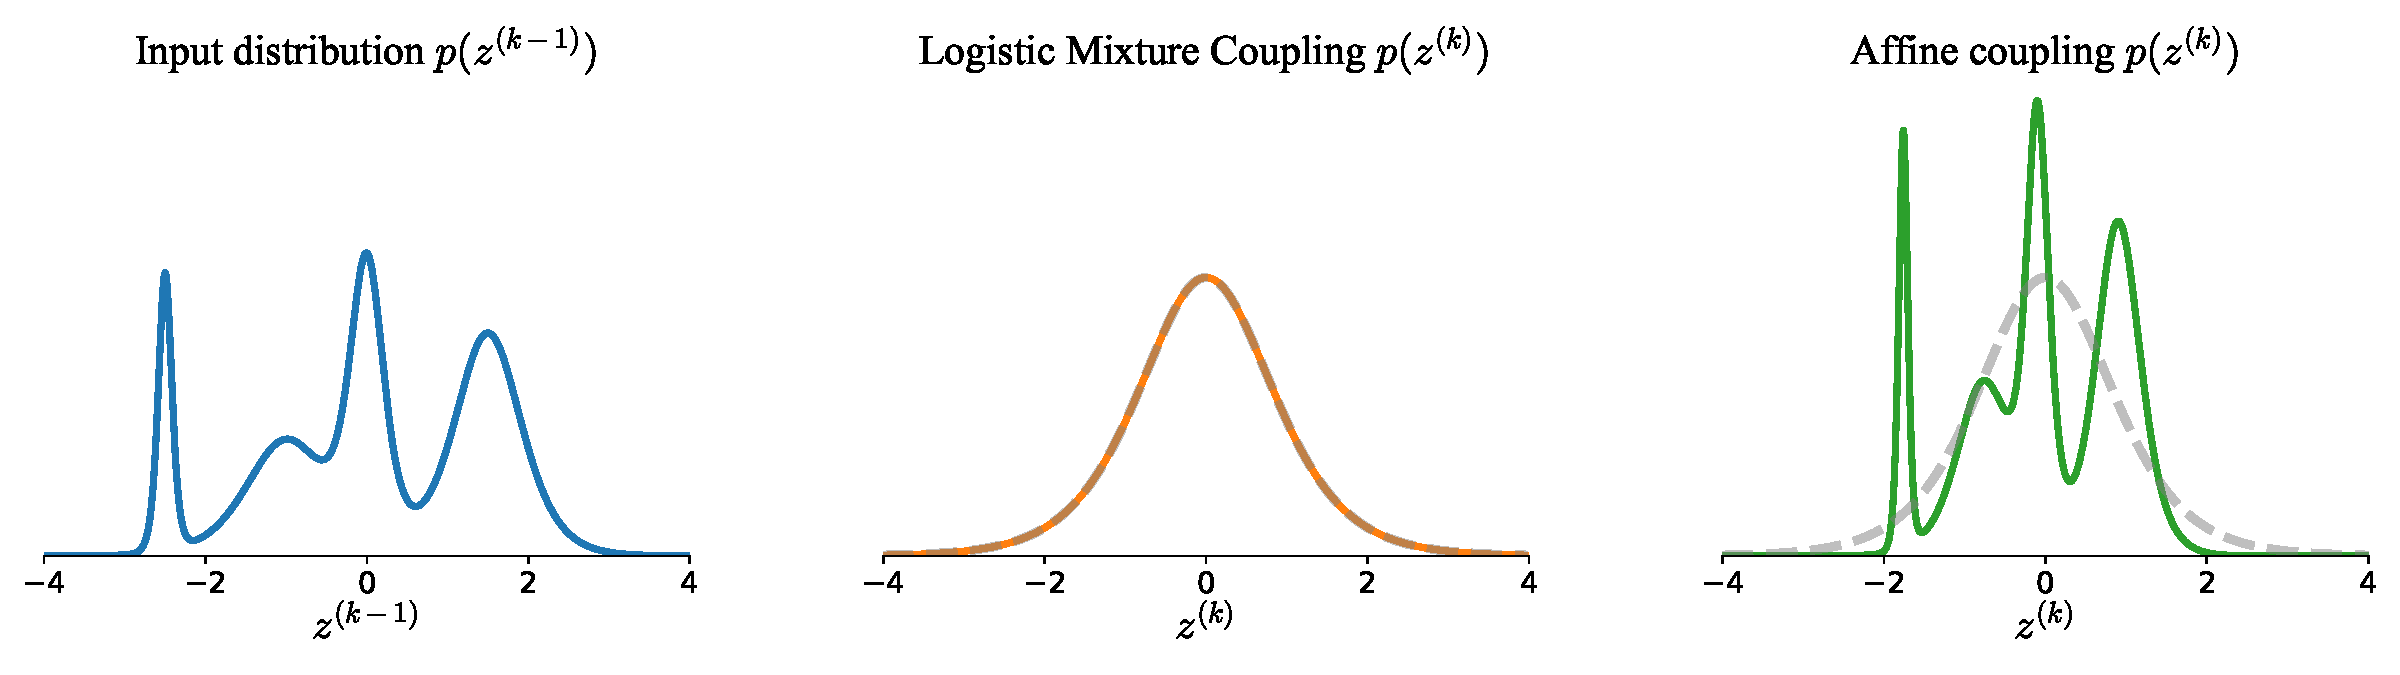
\includegraphics[width=\linewidth]{figures/flow_layer_figures/MoL_logistic_prior_font.pdf}
    \end{subfigure}
    \caption[Comparing affine and logistic mixture coupling layer on single dimension]{Comparing a standard affine coupling layer with a logistic mixture variant on transforming a mixture model to a single mode (shown in gray) in one dimension. While the logistic mixture layer is able to map the input distribution to a single mode, the affine coupling can only change the scaling and mean. Such transformations are crucial for flows as prior distributions have commonly a single mode.}
    \label{sec:background_comparing_coupling_layers}
\end{figure}

\paragraph{Logistic Mixture Coupling} The logistic mixture coupling layer is based on the idea of mapping a distribution of $K$ mixtures back into a single mode. This allows more complex transformations than affine coupling and can especially help for multi-modal input distribution, as visualized in Figure~\ref{sec:background_comparing_coupling_layers}.

The transformation $f$ consists of applying a \ac{CDF} for a mixture of $K$ logistic distributions on $\bm{z}^{(k-1)}_{j+1:d}$. This transformation is followed by an inverse sigmoid to ensure a globally existing inverse of the layer, and a standard affine transformation parameterized by $a$ and $b$. The position $\bm{\mu}$ and scale $\bm{s}$, as well as the mixture components $\pi_{1,...,K}$ of those $K$ logistics are also parameterized by a neural network with $\bm{z}^{(k-1)}_{1:j}$ as input. The full transformation for a single scalar latent variable $z$ with given parameters $\bm{\pi}, \bm{\mu}, \bm{s}, a, b$ is defined as follows:
\begin{equation}
    y = \sigma^{-1}\left(\sum_{i=1}^{K} \pi_i \sigma\left(\frac{z-\mu_i}{\exp(-s_i)}\right)\right)\cdot \exp(a)+b
\end{equation}
where $\sigma$ represents the sigmoid function: $\sigma(x)=\left(1+\exp(-x)\right)^{-1}$.
In general, this coupling layer is not limited to the logistic distribution and could be applied to any mixture model. However, logistics provide a cheap and differentiable \ac{CDF} making them attractive for backpropagation-based optimization. 
The Jacobian determinant can be efficiently calculated based on the probability density function of the logistics.
Inverting the transformation requires the usage of an iterative algorithm like the bisection method because it represents a monotonically increasing function without an analytical inverse.

\subsubsection{Autoregressive flows}
Intuitively, a single coupling layer is limited by the inter-variable interactions it can model as the transformations solely depend on one part of the input. 
Furthermore, the other part of the input is not changed at all requiring multiple coupling layers to be used.
A class of more complex flows that are flexible enough to model any probability distribution while still having a triangular Jacobian are \textit{autoregressive flows}. 
Instead of splitting the input into two parts, autoregressive flows define an order of the latent variables and use all previous elements to calculate the transformation parameters of the next variable:
\begin{eqnarray}
	\bm{z}^{(k)}_{j} & = & f\left(\bm{z}^{(k-1)}_{j};\hspace{1mm} \bm{\Theta}\left(\bm{z}^{(k-1)}_{1:j-1}\right)\right)
\end{eqnarray}
The transformation $f$ can use the same design choices as in coupling layers. 
Networks for modeling the transformation parameters are usually recurrent neural networks or masked feedforward networks which support autoregressive prediction \cite{MaskedAutoregressiveFlow}.
While the forward pass can be parallelized, inverting the flow requires a sequential execution as for calculating $\bm{z}^{(k-1)}_j$, the outputs $\bm{z}^{(k-1)}_{1:j-1}$ need to be determined first. 
Such a sequential calculation significantly slows down the sampling process for which the inverse is required. 
However, the flow could also be flipped such that the inverse is used during training and the forward for sampling. 
Those flows are called \textit{inverse autoregressive flows} \cite{InverseAutoregressiveFlows}, and trade fast sampling for slow density estimation.

\subsubsection{Activation Normalization}

When training deep normalizing flows, initialization must be done carefully as arbitrary transformations with large scaling and/or bias terms can introduce a very high initial KL divergence \cite{NormalizingFlowsOverview}. 
Taking inspiration from normalization layers in standard neural networks, \citet{RealNVP} proposed to apply batch normalization on the outputs of each flow. 
This layer improves the gradient signal throughout the flow and stabilizes scaling-based transformations while keeping the output distribution close to the prior. 
Nevertheless, batch normalization has shown to be noisy for small mini-batches.

As an alternative, \citet{Glow} proposed an \textit{activation normalization} layer which performs an affine transformation using a scale and bias parameter that can be shared across certain dimensions. 
Thereby, the parameters are initialized such that for a randomly selected batch of data, the latent variables after this layer have a zero mean and unit variance. 
Still, the scale and mean parameter are afterwards treated as trainable variables. 
Activation Normalization has shown to stabilize normalizing flows despite their simplicity and is being used in most \acl{SOTA} architectures \cite{Glow, Flow++, FloWaveNet, VFlow, EmielDequantization}.

\subsubsection{Permutation layers}
When using coupling layers, it is important to alternate the input split to allow transformations on all variables. 
This is usually done by permuting the latent variables $\bm{z}$ across a dimension. 
For instance, when modeling images, \citet{RealNVP} reversed the order of the channels before performing a coupling layer.
However, this permutation is predefined and fixed although it is not clear whether this is the optimal split of latent variables for all coupling layers.
To allow a permutation to be learned, \citet{Glow} proposed an invertible 1x1 convolution where the weight matrix is initialized as a random rotation matrix. 
Specifically, the transformation can be formulated as:
\begin{equation}
    \bm{z}^{(k)} = \bm{W}\bm{z}^{(k-1)}
\end{equation}
with $\bm{W}\in\mathbb{R}^{D\times D}$. 
Note that this operation is performed across the dimension that should be permuted (e.g. channels in images).
The transformation is invertible if $\bm{W}$ is invertible itself. 
To guarantee the invertibility of $\bm{W}$, \citet{Glow} suggest representing the weight matrix in its LU decomposition:
\begin{equation}
    \bm{W} = \bm{P}\bm{L}\left(\bm{U} + \text{diag}\left(\bm{s}\right)\right)
\end{equation}
where $\bm{P}$ is a permutation matrix, $\bm{L}$ is a lower triangular matrix with ones on the diagonal, and $\bm{U}$ an upper triangular matrix with zeros on the diagonal. 
The vector $\bm{s}$ is an additional scaling term based on which the Jacobian can be calculated. 
While $\bm{P}$ is fixed after initialization, $\bm{L}$, $\bm{U}$ and $\bm{s}$ are being optimized while enforcing the triangularity of the matrices.
With such a decomposition, the invertible 1x1 convolution enables the optimization of the permutation within a normalizing flow. 
\newpage
\section{Related Work}
\label{sec:related_work}

The following section reviews recent work on modeling discrete data distributions using normalizing flows. 
Specifically, Section~\ref{sec:related_work_dequantization} discusses the concept of \textit{dequantization} to represent ordinal discrete data as a continuous distribution, which is commonly used for normalizing flows trained on image modeling \cite{RealNVP, Glow, Flow++}. 
An alternative, popular generative model for discrete data is the framework of \acfp{VAE} \cite{VAE} that model a lower-bound estimate of the data likelihood. 
Its hybrid versions with a flow-based posterior or prior are reviewed in Section~\ref{sec:related_work_VAE_flow}. 
Additionally, normalizing flows can be directly applied to discrete data by reformulating the change-of-variable formula to discrete inputs, which is presented in Section~\ref{sec:related_work_discrete_flows}.
Finally, Section~\ref{sec:related_work_graph_modeling} reviews recent work on applying normalizing flows to the task of graph modeling.

\subsection{Input Dequantization}
\label{sec:related_work_dequantization}

% A common application and benchmark of normalizing flows has been the modeling and generation of images. Thereby, images are a discretized representation of a real-world scene, as in reality, colors are not limited to discrete pixel values. Directly applying continuous normalizing flows on discrete data will lead to an undesired solution \cite{UriaContPeaks, Theis2015}. As discrete points correspond to delta functions with infinite height in continuous space, the flow would try to fit such delta functions. Therefore, the probability of a value such as $127$ could be close to infinity while $127.1$ has one close to zero. Hence, the likelihood values would be almost meaningless as single data points can reach infinite probabilities.
Applying continuous normalizing flows on discrete data leads to undesired density models where arbitrarily high likelihoods are placed on particular values. This is because discrete data points represent delta peaks in a continuous distribution, and a normalizing flow would place arbitrarily high likelihood to those discrete points making the density function useless \cite{Theis2015, UriaContPeaks}. 
To prevent such degenerated solutions, a common solution is to add a small amount of noise to each discrete value, which is also referred to as dequantization \cite{RealNVP, Flow++, EmielDequantization}. 
Considering $\bm{x}$ as an integer, the dequantized representation $\bm{v}$ can be formulated as $\bm{v}=\bm{x}+\bm{u}$ where $\bm{u}\in[0,1)^D$. 
Thus, the discrete value $1$ is modeled by a distribution over the interval $[1.0, 2.0)$.   \citet{Theis2015} have shown that modeling the dequantized representation, $p_{\text{model}}(\bm{v})$, lower-bounds the modeled discrete distribution $P_{\text{model}}(\bm{x})$, and hence prevents arbitrarily high likelihoods. 
Meanwhile, the flow remains invertible as $\bm{x}+\bm{u}$ constitute disjoint intervals so that each continuous point can be mapped back to exactly one discrete point $\bm{x}$ by finding the next lower whole number for each element $v_i$. 
In summary, modelling the discrete data distribution $P_{\text{data}}(\bm{x})$ by a normalizing flow can be written as:
\begin{eqnarray}
    \label{eqn:related_work_dequantization_uniform}
    % P_{\text{model}}(\bm{x}) = \int_{[0,1)^D} p_{\text{model}}(\bm{x}+\bm{u})\hspace{1mm}d\bm{u} = \E_{\bm{u} \sim [0,1)^D}\left[p_{\text{model}}(\bm{x}+\bm{u})\right] \\
    & & \E_{\bm{x}\sim P_{\text{data}}}\left[\log P_{\text{model}}(\bm{x})\right] \geq \E_{\bm{x}\sim P_{\text{data}}}\E_{\bm{u} \sim [0,1)^D}\left[\log p_{\text{model}}(\bm{x}+\bm{u})\right]
\end{eqnarray}
% following the notation of \citet{Flow++} where $P(x)$ represents the discrete probability distribution, and $p(x)$ the continuous flow-modeled distribution. The vector $\bm{u}$ corresponds to uniform noise which is sampled independently for all $D$ dimensions of the data.

Nevertheless, by representing discrete values as uniform distributions, the flow is required to model unit hypercubes around the data points. This is difficult for smooth transformation to capture and has shown to harm the modeling capacity \cite{EmielDequantization} (see Figure~\ref{fig:related_work_dequantization_techniques}). Dequantization has therefore been extended to more sophisticated, learnable distributions beyond uniform in a variational framework. In particular, the uniform distribution can be replaced by a learned distribution $q(\bm{u}|\bm{x})$ with support over $\bm{u}\in[0,1)^D$ by rewriting Equation~\ref{eqn:related_work_dequantization_uniform} as follows:
\begin{equation}
    \label{eqn:related_work_dequantization_variational}
    % P(\bm{x}) = \int_{[0,1)^D} q(\bm{u}|\bm{x})\frac{p(\bm{x}+\bm{u})}{q(\bm{u}|\bm{x})} d\bm{u} = \E_{\bm{u} \sim q(\bm{u}|\bm{x})}\left[\frac{p(\bm{x}+\bm{u})}{q(\bm{u}|\bm{x})}\right]
    \E_{\bm{x}\sim P_{\text{data}}}\left[\log P_{\text{model}}(\bm{x})\right] \geq \E_{\bm{x}\sim P_{\text{data}}}\E_{\bm{u}\sim q(\cdot|\bm{x})}\left[\log \frac{p_{\text{model}}(\bm{x}+\bm{u})}{q(\bm{u}|\bm{x})}\right]
\end{equation}
The distribution $q(\bm{u}|\bm{x})$ is commonly implemented by a normalizing flow conditioned on the input $\bm{x}$ (i.e. the applied transformations are influenced by $\bm{x}$). 
The constraint of having a support only over the unit hypercube $[0,1)^D$ can be fulfilled by applying a sigmoid activation function on the final output of the normalizing flow. 
Currently, models with variational dequantization like autoregressive models constitute the \acl{SOTA} for flow-based image modeling \cite{VFlow, EmielDequantization}. 

Such dequantization techniques, however, cannot be as simply applied on nominal discrete data where the values represent categories with no intrinsic order. 
Treating these categories as integers for dequantization biases the data to a non-existing order, and consequently makes the modeling task significantly harder.
Therefore, the application of variational dequantization has been mostly limited to ordinal discrete data.

\begin{figure}[t!]
    \centering
    \begin{subfigure}{0.4\textwidth}
        \centering
        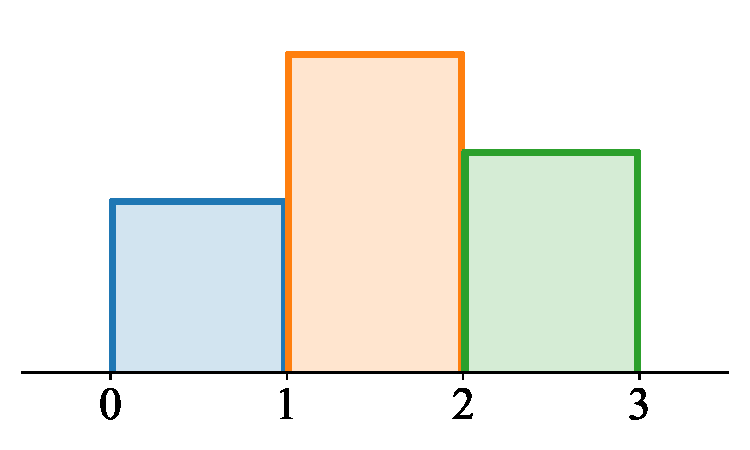
\includegraphics[width=0.65\textwidth]{figures/related_work_figures/dequant.pdf}
        \caption{Uniform dequantization}
    \end{subfigure}
    \begin{subfigure}{0.4\textwidth}
        \centering
        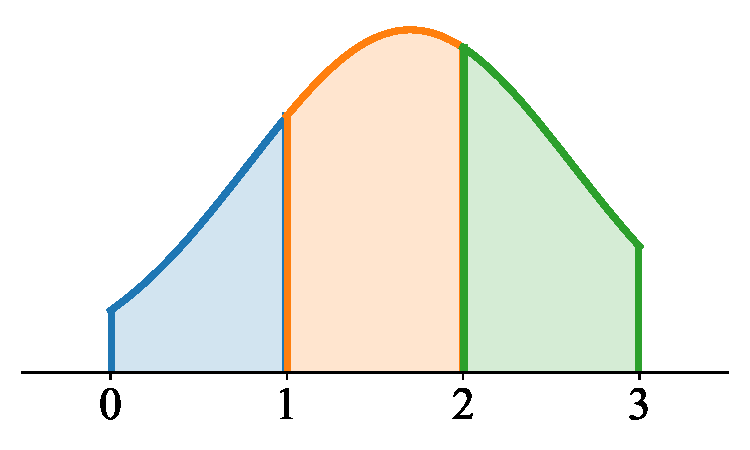
\includegraphics[width=0.65\textwidth]{figures/related_work_figures/var_dequant.pdf}
        \caption{Variational dequantization}
    \end{subfigure}
    \caption[Uniform and variational dequantization]{Visual comparison between (a) uniform and (b) variational dequantization for the integers $0$ (blue), $1$ (orange) and $2$ (green). The continuous representation shows the dequantization distribution of $x+u$ for a single dimension. While the uniform case requires the flow to model sharp edges between integers, variational dequantization allows for more flexible distributions and simplifies the modeling task for the consecutive normalizing flow.}
    \label{fig:related_work_dequantization_techniques}
\end{figure}

%%% - SUBSECTION - %%%
\subsection{Flow-based Variational Auto-Encoders}
\label{sec:related_work_VAE_flow}

In contrast to normalizing flows, \acp{VAE} \cite{VAE} can handle discrete data without additional overhead. This is because the \ac{VAE} framework models the following variational lower bound of the data likelihood, called \ac{ELBO}:
\begin{equation}
    \log p(\bm{x}) \geq \E_{q_{\phi}(\bm{z}|\bm{x})}\left[\log p_{\theta}(\bm{x}|\bm{z}) + \log p_{\theta}(\bm{z}) - \log q_{\phi}(\bm{z}|\bm{x})\right]
\end{equation}
The likelihood $p_{\theta}(\bm{x}|\bm{z})$ represents the decoder (i.e. decoding latent variable $\bm{z}$ to $\bm{x}$), while the (approximate) posterior $q_{\phi}(\bm{z}|\bm{x})$ is the encoder (i.e. encoding $\bm{x}$ into latent variable $\bm{z}$). The difference between the true log-likelihood and the ELBO is the KL divergence between the approximate posterior $q_{\phi}(\bm{z}|\bm{x})$ and the true (unknown) posterior $p_{\theta}(\bm{z}|\bm{x})$: $D_{\text{KL}}(q_{\phi}(\bm{z}|\bm{x})||p_{\theta}(\bm{z}|\bm{x}))$.
Both the encoder and decoder are usually implemented by deep neural networks, which, in comparison to normalizing flows, do not have to be invertible. Thus, a mapping from discrete space to continuous is easily possible by predicting a suitable distribution for $\bm{z}$. 

The prior $p_{\theta}(\bm{z})$ is often assumed to be a standard normal distribution in the \ac{VAE} \cite{VAE} but also other distributions such as Mises-Fisher on hyperspherical space \cite{VAEHyperspherical} or mixture-based approaches \cite{VAESemiSupervised, VampPrior} have been proposed. The output of the encoder $q_{\phi}(\bm{z}|\bm{x})$ is usually designed to fit the prior distribution. For a Gaussian prior with diagonal covariance, the encoder predicts a mean and variance per latent dimension. This allows an efficient computation of the KL divergence between prior and encoder, but limits the flexibility of the encoder which is needed to accurately fit the true posterior $p_{\theta}(\bm{z}|\bm{x})$. One approach for increasing flexibility is applying a normalizing flow on top of the output of the encoder \cite{InverseAutoregressiveFlows}. Those flow transformations are parameterized by the features of the encoder, to allow simpler, input-dependent transformations. Figure~\ref{fig:related_work_VAE_flow_hybrids_1} visualizes the approach. The usage of various kinds of normalizing flows has been explored in the setting of a \ac{VAE}, including inverse autoregressive flows \cite{InverseAutoregressiveFlows} and Sylvester normalizing flows \cite{SylvesterNF}, a generalization of planar flows.

\begin{figure}[t!]
    \centering
    \begin{subfigure}{0.53\textwidth}
        \centering\vspace{8mm}
        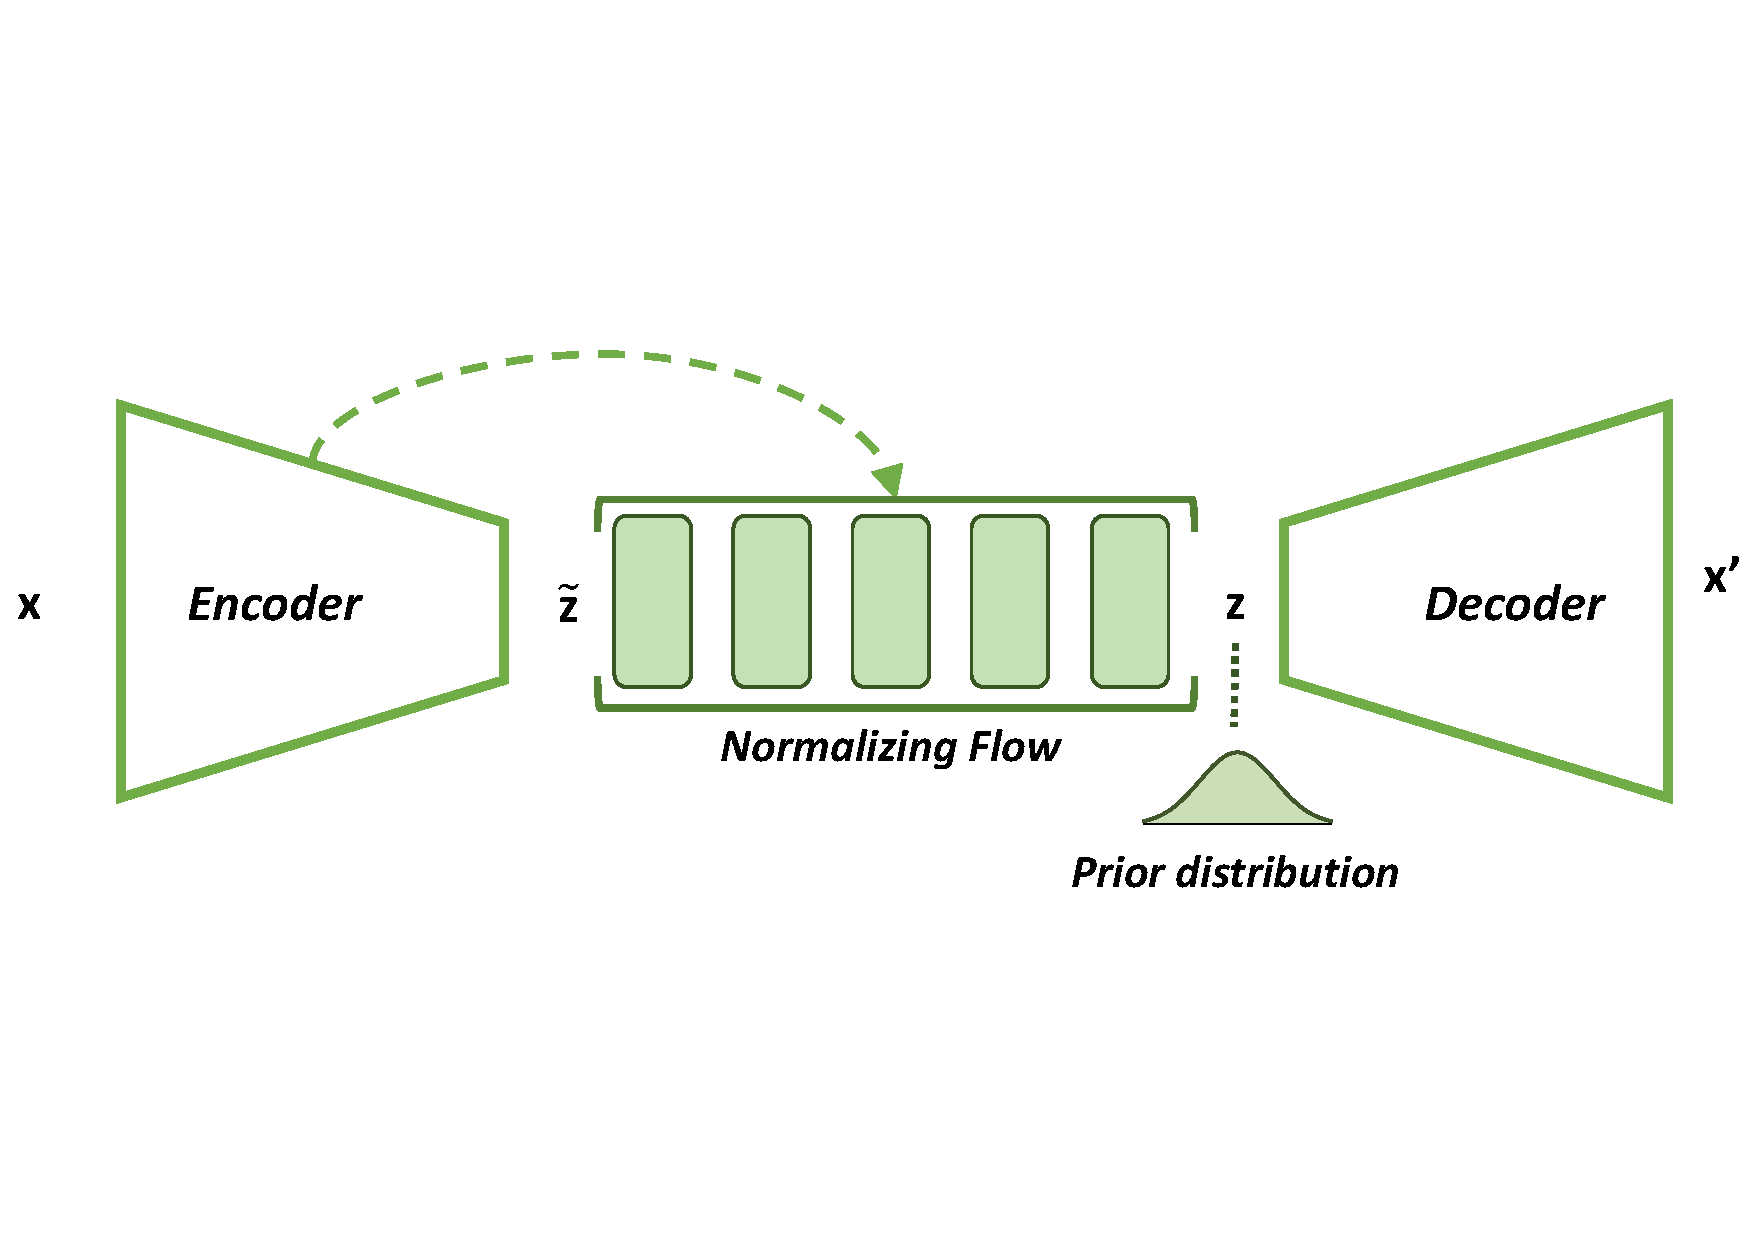
\includegraphics[width=\linewidth]{figures/related_work_figures/VAE_Flow_1.pdf}\vspace{8mm}
        \caption{Flow-based encoder}
        \label{fig:related_work_VAE_flow_hybrids_1}
    \end{subfigure} \hspace{10mm}
    \begin{subfigure}{0.39\textwidth}
        \centering
        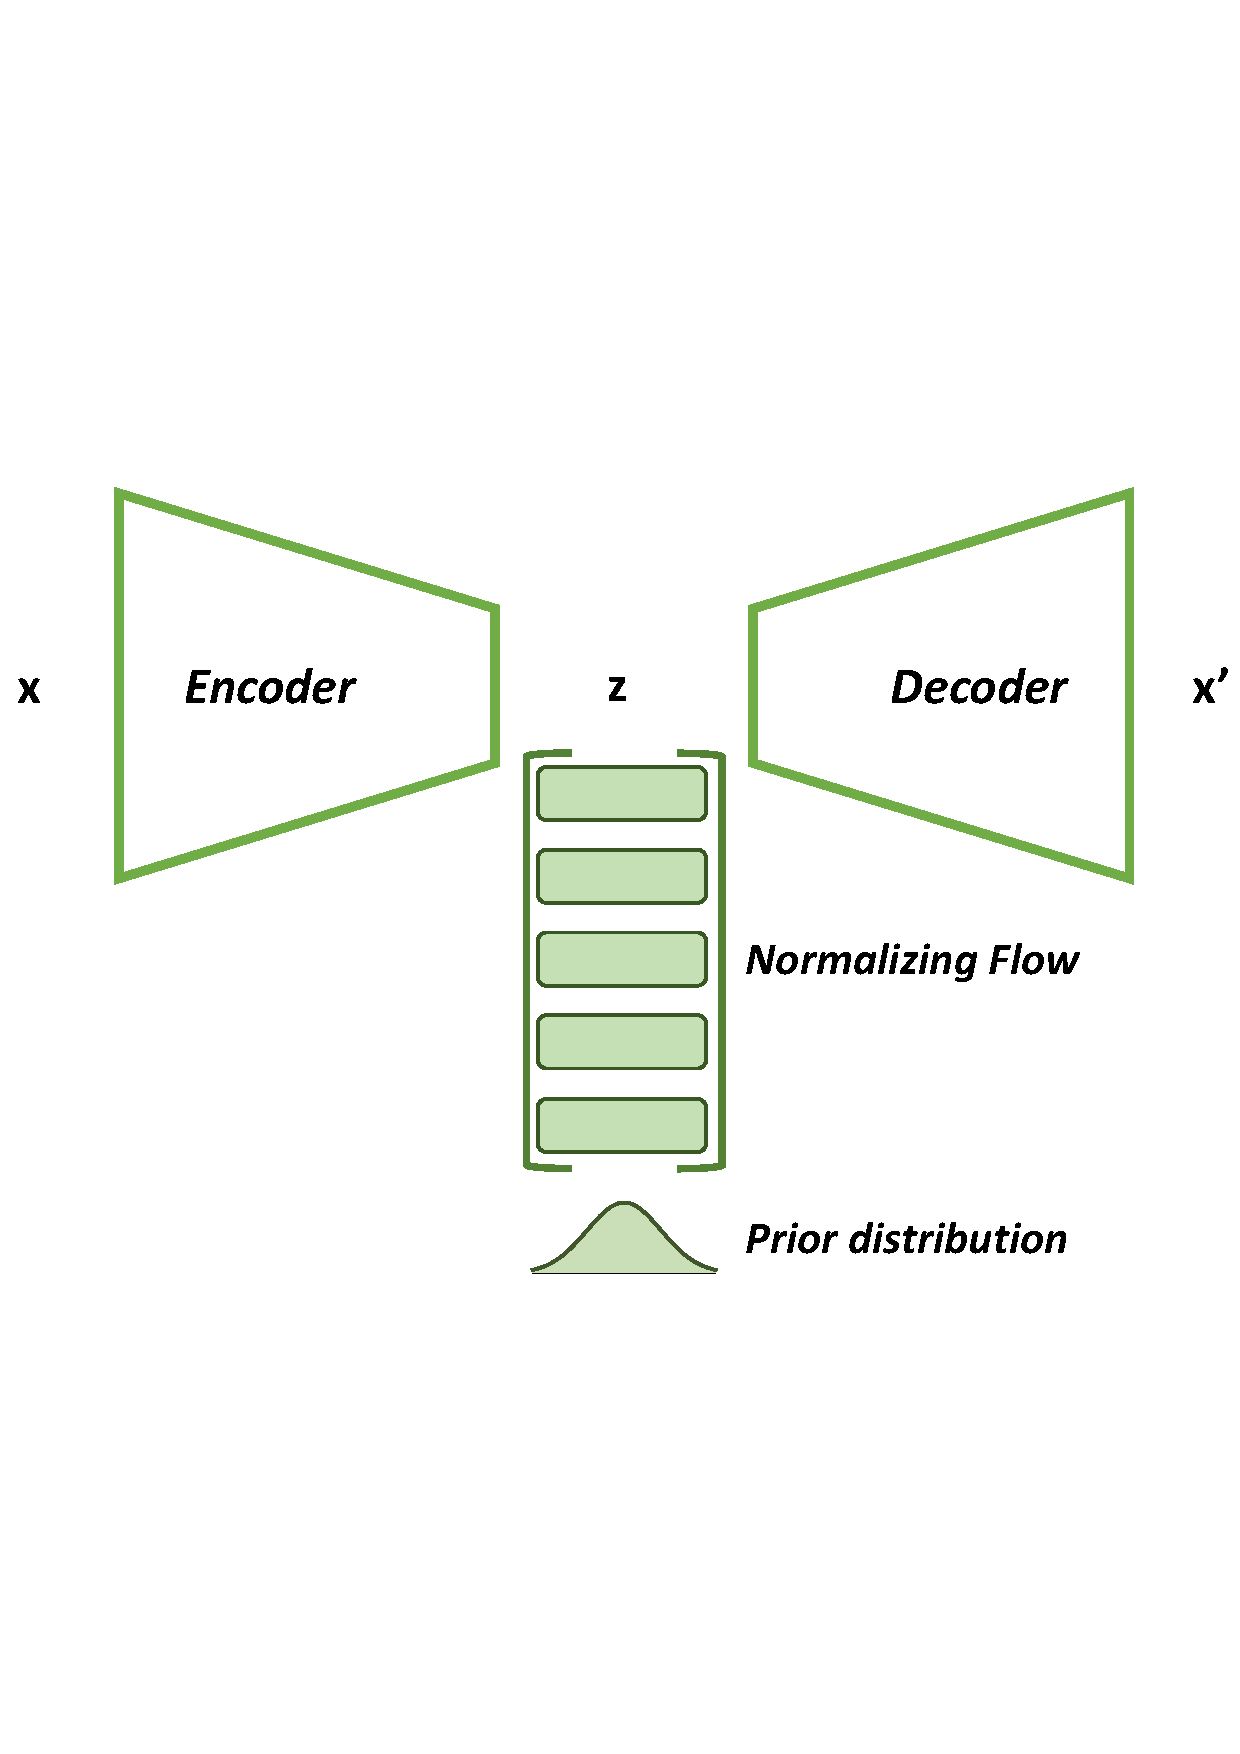
\includegraphics[width=\linewidth]{figures/related_work_figures/VAE_Flow_2.pdf}
        \caption{Flow-based prior}
        \label{fig:related_work_VAE_flow_hybrids_2}
    \end{subfigure}
    \caption[Hybrid model variants for combining VAEs with normalizing flows]{Hybrid model variants for combining \ac{VAE} with normalizing flows. (a) The encoder's distribution can be extended by applying a normalizing flow on top of a simpler output distribution $q_{\phi}(\bm{z}'|\bm{x})$. Features from the encoder parameterize the flow. The output of the flow, representing $\bm{z}$, is trained to follow the prior distribution $p(\bm{z})$. (b) The prior $p(\bm{z})$ can itself be a normalizing flow allowing a more flexible prior distribution. The encoder and decoder are usually smaller in this case as the complexity is moved into the prior.}
    \label{fig:related_work_VAE_flow_hybrids}
\end{figure}

A second approach, called Latent Normalizing Flows \citet{SemiDiscreteNFSequence}, is to model the prior $p(\bm{z})$ by a normalizing flow instead (see Figure~\ref{fig:related_work_VAE_flow_hybrids_2}). 
In this setup, the main modeling complexity is moved into the normalizing flow while the encoder and decoder networks are usually simplified. 
As a result, the KL divergence between the approximate and true posterior is expected to be considerably lower and pushes the evidence lower bound closer to the true likelihood. 
This motivation was verified by experiments of \citet{SemiDiscreteNFSequence} where the reconstruction loss was close to zero while the prior likelihood dominated the objective. 
Although the flow requires $\bm{z}$ to be continuous, the input $\bm{x}$ can be discrete. 
Nevertheless, experiments on language modeling showed that even a 5 layer autoregressive flow was not able to meet the single-layer RNN baseline. 
The encoder and decoder were both modeled by a two-layer bidirectional LSTM \cite{LSTM}.
This suggests that the added complexity of the encoder and decoder actually harms the modeling capability of the normalizing flow, and we verify this issue by experiments in Section~\ref{sec:experiments_language_modeling}.
% \TODO{This part needs to be clear and convincing. Currently it is not...}

% Nevertheless, the \ac{VAE} framework only models a lower bound instead of an exact likelihood estimate as in the standard setup for normalizing flows. Furthermore, the decoder can suffer from posterior collapse ignoring the latent code \cite{VAEPosteriorCollapse}. This has even been the case for shallow decoder networks used by \cite{SemiDiscreteNFSequence}.

%%% - SUBSECTION - %%%
\subsection{Discrete Normalizing Flows}
\label{sec:related_work_discrete_flows}

Recent works by \citet{TranDiscreteFlows}, \citet{IntegerNF} and \citet{IDF++} have explored the approach of applying normalizing flows directly on discrete data. In particular, the rule of change of variable for an invertible function $f$ can be formulated on discrete input data as follows:
\begin{equation}
    \label{eqn:change_of_variable_discrete}
    p(\bm{z}'=z') = p(\bm{z}=f^{-1}\left(z'\right))
\end{equation}
Note that in contrast to Equation~\ref{eqn:related_work_change_of_variables}, the discrete formula does not have a log-determinant Jacobian which takes the volume change into account. This is because in a discrete space there exists no volume which could be modified. 
Furthermore, two inputs cannot be mapped to the same output as otherwise, the function is not invertible anymore. 
Hence, the determinant of the Jacobian will always be one.

Designing the invertible function $f$ can be done similarly as for the continuous case. For instance, \citet{IntegerNF} proposed to discretize the transformation by rounding the additive term of the affine coupling layer:
\begin{equation}
    \bm{z}^{(k)}_{i} = \bm{z}^{(k-1)}_{i} + \big\lfloor\bm{\mu}_{\theta,i}\big\rceil
\end{equation}
where $\lfloor\cdot\rceil$ denotes the rounding operator to the nearest integer. 
The transformation can be defined as $f:\mathbb{Z}^{d}\to\mathbb{Z}^{d}$. 
Since the rounding operator is similar to a step function and has zero gradients for almost any input, a straight-through estimator \cite{STEGradientEstimator} is applied.
This estimator effectively skips the rounding operator during backpropagation and assumes a unit gradient everywhere: $\nabla_{x}\lfloor x\rceil = 1$.
However, note that this introduces gradient bias as backpropagation is not performed on the ``true'' gradients. 

The coupling layers introduced by \citet{IntegerNF} work well on integers, but in the case of categorical variables, the input space is bounded to a finite, discrete set on which the transformations have to operate. 
For this setup, \citet{TranDiscreteFlows} proposed the following affine coupling layer:
\begin{equation}
    \bm{z}^{(k)}_{i} = (\bm{\mu}_{\theta,i} + \bm{\sigma}_{\theta,i} \odot \bm{z}^{(k-1)}_i) \hspace{-2mm}\mod{M}
\end{equation}
where $\bm{\mu}_{\theta,i}$ and $\bm{\sigma}_{\theta,i}$ are functions with discrete outputs parameterized by $\theta$, and $\bm{\mu}_{\theta,i}, \bm{\sigma}_{\theta,i}, \bm{z}^{(k-1)}_{i} \in \llbracket0\mathrel{{.}\,{.}}\nobreak M-1\rrbracket$ where $M$ denotes the number of categories in the discrete distribution.
The modulo operator ensures that the output space is in the same finite, discrete set as the input. 
For the scaling transformation to be invertible, $\bm{\sigma}_{\theta,i}$ and $M$ have to be coprime. 
As $M$ is usually fixed by the task and/or input distribution, $\bm{\sigma}_{\theta,i}$ has been set to 1 for simplicity in most experiments. 

To predict the discrete transformation parameters $\bm{\mu}_{\theta,i}$ and $\bm{\sigma}_{\theta,i}$, \citet{TranDiscreteFlows} proposed to use a standard softmax output and discretize it by taking the argmax over logits. 
However, to maintain a fully differentiable architecture, the argmax operator is replaced by the Gumbel softmax \cite{GumbelSoftmax1, GumbelSoftmax2} using a straight-through estimator \cite{STEGradientEstimator} during backpropagation:
\begin{equation}
    \frac{\partial \bm{\mu}_{\theta,i}}{\partial \theta} \approx \frac{\partial}{\partial \theta} \text{softmax}\left(\frac{\theta}{\tau}\right)
\end{equation}
The temperature parameter $\tau$ controls the trade-off between bias of the gradient estimator and vanishing gradients. 
If $\tau\to 0$, the softmax becomes an argmax, so that the bias is reduced to zero while the gradients vanish and harm learning. 
When $\tau$ is large, the bias of the gradient estimator becomes large due to the considerable difference between the argmax and softmax. 
Keeping the gradient estimator bias low is especially crucial for deep normalizing flows as the bias can aggregate over layers and destabilize the training \cite{EmielDequantization}.

In experiments on the task of language modeling, discrete normalizing flows have shown to perform on par with autoregressive models such as LSTM while allowing a fully parallelized generation process. 
Moreover, discrete flows outperformed the flow-based \ac{VAE} approach by \citet{SemiDiscreteNFSequence}. % , underlining that operating on a discrete space is not a drawback for a normalizing flow
Nevertheless, the argmax approximations prevent the number of categories to be scaled up to more than 200 as otherwise, the bias of estimator becomes too large \cite{GumbelSoftmax1, GumbelSoftmax2}.

Despite the success of discrete flows on the experiments deducted by \citet{TranDiscreteFlows}, several works have pointed out the limitations of such flows besides gradient approximation \cite{SemiDiscreteNFSequence, NormalizingFlowsOverview2, IDF++}. 
In particular, due to the invertibility constraint in Equation~\ref{eqn:change_of_variable_discrete}, transformations in discrete flows can only model permutations of the input set \cite{SemiDiscreteNFSequence}.
This significantly limits the modeling capability in low-dimensional spaces and prevents the flow from learning arbitrary distribution with factorized base distributions as it is the case for continuous flows.
For example, suppose we have the following distribution over $\bm{x}\in\{0,1\}^{2}$:
\begin{table*}[ht!]
    \centering
    \begin{tabular}{ccc}
         & $x_2=0$ & $x_2=1$ \\
         \midrule
         $x_1=0$ & $0.1$ & $0.2$ \\
         $x_1=1$ & $0.3$ & $0.4$ \\
         \bottomrule
    \end{tabular}
\end{table*}

Within the $4!$ possible permutations, there exists no invertible transformation from $\bm{x}$ to $\bm{z}\in\{0,1\}^{2}$ such that $p_z(\bm{z})$ can be expressed as by two factorized base distributions: $p_x(\bm{x})=p_z(\bm{z})=p_z(z_1)p_z(z_2)$.
Although \citet{IDF++} argue that by expanding the domain of $\bm{x}$ and $\bm{z}$ to $\{0,1,2,3\}^{2}$, the probability distribution can be modeled by a discrete flow, this only generalizes by expanding the domain to $M^{d}$ elements which is infeasible for real-world data like text.
Therefore, those flows have to rely on strong base distributions such as autoregressive ones, which inherently slow down sampling.
On the other hand, normalizing flows on continuous data can model any input distribution with the requirement of using sufficiently complex transformations \cite{NormalizingFlowsOverview, NormalizingFlowsOverview2}. 


\subsection{Graph modeling}
\label{sec:related_work_graph_modeling}

\begin{figure}[b!]
    \centering
    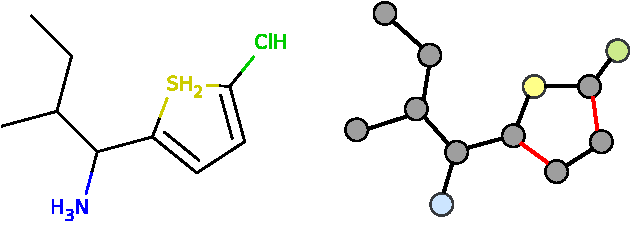
\includegraphics[width=0.65\textwidth]{figures/related_work_figures/molecule_graph.pdf}
    \caption[Visualization of molecule graph]{In graph-based molecule generation, the chemical representation (left) is translated into a graph (right) by encoding atoms as nodes and bonds as edges. Node and edge categories are visualized by different colors. The task is to model a distribution of valid graphs which is coherently difficult as the models have to consider edges between any pairs of nodes. Molecule taken from the Zinc250k dataset \cite{Zinc250k}.}
    \label{fig:related_work_graph_molecule}
\end{figure}

Modeling and generating graphs is a crucial application in areas such as biology and chemistry, and deep learning approaches have recently gained interest in such tasks \cite{GraphRNN, GraphOverview1, GraphOverview2, GraphAF}.
A graph $\mathcal{G}=(V,E)$ is defined by a set of vertices or nodes $V$, and a set of tuples representing edges $E$ between vertices. 
A common alternative representation of the edges is the adjacency matrix whose elements indicate whether a pair of nodes is connected by an edge or not.
Both the nodes and edges can have attributes that are often categorical and need to be predicted as well besides the overall graph structure.
The first generation models on graphs have been autoregressive \cite{GraphRNNAttention, GraphRNN, MolecularRNN}, generating nodes and edges in sequential order. 
While being efficient in memory, they are slow in sampling as the generation time scales quadratically with the number of nodes (for $N$ nodes, there are $N(N-1)/2$ edges to predict).

However, a considerable drawback of autoregressive models on graphs is that they assume an order in the set of nodes although the nodes are not a sequence. 
Permuting the nodes in the set while adjusting the edges accordingly represents the exact same graph.
Therefore, a generative model should ideally be permutation invariant concerning the order in the set as well to automatically assign the same likelihood to each ordering of a graph. 
Nonetheless, autoregressive models are sensitive to the order assigning the same graph with different orderings different likelihood values.
Furthermore, previous work has shown that introducing an order to an actually unordered set can lead to a strong bias and harms the performance \cite{OrderMatters}.

Normalizing flows, on the other hand, can perform generation in parallel allowing them to build a permutation invariant density model.
The first application of normalizing flows for graph generation was introduced by \citet{GraphNF}, where a flow models the latent node representations of a pretrained autoencoder. 
While the proposed flow is permutation invariant, the model does not support node or edge attributes.
Recent works of GraphNVP \cite{GraphNVP} and GraphAF \cite{GraphAF} showed applications on molecule generation where nodes represent atoms and edges different types of bonds between the atoms (see Figure~\ref{fig:related_work_graph_molecule}). 

GraphNVP consists of two separate flows, one for modeling the adjacency matrix and a second for modeling the node types. 
Although allowing parallel generation, the model is sensitive to the node order due to two design choices.
Firstly, the coupling layers in GraphNVP transform the latent variables of a single node, which is decided based on an assumed order, while using all others as input.
Hence, permuting the nodes represents a different graph for the model. 
Secondly, the feature networks in the coupling layers are multi-layer perceptrons that flatten the adjacency matrix into a vector.
Thus, the predicted transformation parameters are sensitive to the node order and fixed to a specific graph size (the model cannot generate graphs larger than in the training set).
In comparison, GraphAF combines autoregressive models and normalizing flows by applying autoregressive flows on the graph structure. 
Although having the same drawbacks as autoregressive models, it provides a latent space which can be used for tasks like drug discovery \cite{MolecularRNN, GraphAF} and outperforms GraphNVP by a considerable margin.

To embed the discrete, categorical node and edge attributes into continuous space, both flows use standard uniform dequantization on a one-hot representation of its categories.
In this work, we use a variational inference framework instead for the mapping to continuous values. 
Using this representation, we can design a fully permutation-invariant normalizing flow on graphs, called GraphCNF, which assigns an equal likelihood to any permutation of the nodes.


Variational autoencoders have also been proposed for latent-based graph generation \cite{GraphVAE, GraphVAEConstrained, GraphVAEConstrained2, JunctionTreeVAE}. 
Usually, an encoder transforms the discrete graph structure into latent Gaussian variables of fixed size, based on which a decoder reconstructs the graph by predicting the probability of each edge for a fully connected graph. 
To allow the decoder to predict any order of nodes and edges, the reconstruction loss is based on a graph matching algorithm between the input and output.
As this matching can be expensive to compute and is non-differentiable, most recent work has focused on autoregressive decoders that are sensitive to node orders \cite{JunctionTreeVAE, GraphVAEConstrained2}.
% they model a lower bound of the true likelihood.%


% \subsubsection{Review of related work}
% \label{sec:experiments_graph_generation_related_work}

% The first generation models on graphs have been autoregressive. \citet{GraphRNN} introduced GraphRNN, which generates nodes and edges in sequential order. At each inference step, a node is sampled based on the current subgraph structure. Afterward, the edges of the generated node with any other node are created, which is again performed autoregressively. Multiple variants of this model have been proposed, mostly focusing on increasing its expressiveness \cite{MolecularRNN} or memory efficiency to scale up to graphs with thousands of nodes \cite{GraphAttentionNetwork}. However, one of its limitations is the slow generation as it scales with $\mathcal{O}(N^2)$ where $N$ is the number of nodes.

% For faster generation, \citet{GraphVAE} proposed to use \acl{VAE}s on graphs. Specifically, an encoder transforms the discrete graph structure into latent Gaussian variables of fixed size. Based on this latent representation, a decoder reconstructs the graph by predicting the probability of each edge for a fully connected graph. To allow the decoder to predict any order of nodes and edges, the reconstruction loss is based on a graph matching algorithm.

% Applying normalizing flows for the task of graph generation has first been introduced by \citet{GraphNF}. Their approach consists of two steps, of which the first is to train a standard autoencoder on reconstructing graphs. Each node is encoded to an arbitrary feature vector, and for decoding the adjacency matrix, the cosine similarity is used between those vectors. The second step is to learn the distribution of the encoded node feature vectors by a normalizing flow assuming a fully connected graph in the coupling layers. Note that this approach focused on plain graphs without node or edge properties.

% \citet{GraphNVP} extended this approach solely using a normalizing flow to learn a mapping from the graph to latent space. Their model, called GraphNVP, applies coupling layers on node representations which are based on standard dequantization as used in images \cite{RealNVP}. The layers use a \ac{RGCN} \cite{RGCN} based on the adjacency matrix to be permutation invariant. In a second step, the adjacency matrix itself is transformed into a latent space. However, each row of the adjacency matrix is transformed sequentially increasing the number of flows to 38 and breaking the invariance.

% In a similar manner, \citet{GraphAF} uses an autoregressive flow to generate new molecule graphs. Combining the ideas of GraphRNN and GraphNVP

% \begin{itemize}
%     \item \citet{GraphRNN} (Graph RNN): Recurrent Neural Networks trained to generate graphs. Efficient in-memory usage compared to one-shot approaches, variants of this model can generate large graphs up to thousands of nodes \cite{GraphRNNAttention}.\\
%     \textit{Limitations}: Autoregressive although there is no clear ordering in a graph, and slow in generation
%     \item \citet{GraphNF} (Graph Normalizing Flow): First normalizing flow on graphs. It is build up by a (slightly noisy) auto-encoder, and on its output, a normalizing flow is trained. Training is a two-step process (first train auto-encoder, afterward train flow). \\
%     \textit{Limitations}: Does not consider node- and edge-types. Only predicts a binary adjacency matrix with no node specification. NF in general limit the size of the graph due to its one-shot sampling
%     \item \citet{GraphNVP} (GraphNVP): Graph normalizing flows in the context of molecule generation. Predicts the first adjacency matrix, and uses it to predict the node types. A row-mask is used in the coupling layers.\\
%     \textit{Limitations}: Not permutation invariant, uses simple dequantization and is almost autoregressive for the adjacency matrix and node prediction (one row at a time, overall 38 flows for adjacency matrix).
%     \item \citet{GraphAF} (GraphAF): Combines RNN and Flows to an autoregressive graph normalizing flow. Uses a breadth-first search to determine the (unique) ordering of the nodes. Current \ac{SOTA} on molecule generation.\\
%     \textit{Limitations}: Autoregressive, uses simple dequantization and very task specific 
% \end{itemize}
\newpage
\section{Categorical Normalizing Flows}
\label{sec:methodology}

The review of related work has shown that while normalizing flows on categorical distribution exist, they are limited in their expressiveness due to discretizing the change of variable formula.
Continuous normalizing flows, on the other hand, are significantly more powerful.
Motivated by these limitations, we present Categorical Normalizing Flows that jointly learn an encoding distribution to continuous space for categorical data and a consecutive normalizing flow on this continuous representation.
We discuss the details of this approach in Section~\ref{sec:methodology_CNF}.
In the second part, Section~\ref{sec:methodology_GraphCNF}, we introduce GraphCNF, a Categorical Normalizing Flow on graph modeling which is permutation-invariant to the node order. 

\subsection{Continuous Normalizing Flows on Categorical Data}
\label{sec:methodology_CNF}

We define $\bm{x}$ to be a multivariate, nominal discrete random variable, where each element $x_i$ is a categorical variable of $K$ categories with no intrinsic order.
Our goal is to learn the joint probability mass function, $P_{\text{model}}(\bm{x})$, via a normalizing flow.
As normalizing flows originally constitute a class of continuous transformations, it is not directly possible to rely on them for modeling $P_{\text{model}}(\bm{x})$. Instead, we propose to learn a continuous latent space 
in which each categorical choice of a variable $x_i$ maps to one distribution of a continuous variable $\bm{z}_i \in \mathbb{R}^{d}$. 
Thereby, we want to have the following properties:
\begin{itemize}
	\item The continuous distributions corresponding to different categories should be non-overlapping to preserve unique decoding, similar to current dequantization methods. Specifically, the latent space is ideally partitioned into $K$ regions, one for each category. This ensures that no information is lost when mapping the discrete data to continuous values.
	\item In contrast to integers, categories do not have an intrinsic order which would provide a natural positioning of the non-overlapping volumes.
	However, there usually exist (hidden) relations between the categories which are beneficial to represent in the encoding.
	Thus, the positioning of the volumes and distributions per category need to be jointly optimized with the continuous flow $p_{\text{model}}(\bm{z})$ instead of pre-specified.
	\item Relations between data points are usually represented by distance in continuous space. Categories can have several multi-dimensional relations as it is the case for words and their meaning. To encode those relations into the latent space, a single dimension is not sufficient as it cannot represent all the different forms of relations. Thus, the encoding distribution needs to support an arbitrary number of dimensions for $\bm{z}_i$.
\end{itemize}
In summary, the optimal encoding distribution would learn a partitioning of the continuous latent space into $K$ volumes, each representing one category with a flexible distribution within this part.

\subsubsection{Encoding categorical data into continuous latent space}

In order to find such a function, we propose to learn a flexible encoding distribution $q(\bm{z}|\bm{x})$ by simultaneously optimizing a decoder $p(\bm{x}|\bm{z})$ for the reverse mapping. 
This allows us to jointly optimize the encoding of the categorical data with the normalizing flow on the continuous representation. 
A common framework for learning such an encoder-decoder structure on distributions is variational inference \cite{VAE, NormalizingFlowsFundamentals}. 
However, variational inference in the form as presented above has two drawbacks. 
Firstly, defining a joint decoder distribution does not fulfill our desired property of partitioning the latent space. 
Instead, the encoder-decoder model will compress the information as the decoder can infer categories from other continuous variables, which also leads to overlaps in distributions per category. 
However, we want the interaction of the variables to be learned in the normalizing flow to utilize its parallel sampling and exact density evaluation.
Secondly, $p(\bm{x}|\bm{z})$ represents an approximate posterior of the likelihood $q(\bm{z}|\bm{x})$. The difference between the true and approximate posterior is the KL-divergence $D_{KL}(p(\bm{x}|\bm{z})||q(\bm{x}|\bm{z}))$, which cannot be determined as $q(\bm{x}|\bm{z})$ is unknown.
Thus, we can only model a lower bound which tends to increasingly diverge with the true posteriors' complexity \cite{VAEDeeperUnderstanding, VAEAdvances}. 

To overcome these issues, we propose to simplify the decoder by factorizing the posterior: $p(\bm{x}|\bm{z})=\prod_i p(x_i|\bm{z}_i)$. 
This limits the variational inference framework to a toolkit for learning the optimal partitioning of the latent space. 
Factorizing the posterior distribution means that we assume independence between the categorical variables given their learned continuous encodings. 
Therefore, any interaction between the categorical variables $\bm{x}$ must be learned inside the normalizing flow.
On the other hand, the encoder $q(\bm{z}|\bm{x})$ is being optimized to provide suitable representations of the categorical variables to the flow while separating the different categories in latent space to improve the decoding. The KL divergence between true and approximate posterior is also expected to be close to zero as the posterior becomes almost deterministic. 
Overall, our objective becomes:
\begin{equation}
	\E_{\bm{x}\sim P_{\text{data}}}\left[\log P_{\text{model}}(\bm{x})\right] \geq \E_{\bm{x}\sim P_{\text{data}}}\E_{\bm{z}\sim q(\cdot|\bm{x})}\left[\log \frac{p_{\text{model}}(\bm{z}) \prod_i p(x_i|\bm{z}_i)}{q(\bm{z}|\bm{x})}\right]
\end{equation}
We refer to this framework as \emph{Categorical Normalizing Flows}. In contrast to dequantization in Equation~\ref{eqn:related_work_dequantization_variational}, the continuous encoding $\bm{z}$ is not bounded by the domain of the encoding distribution. 
Instead, the partitioning is jointly learned with the model likelihood. 
Furthermore, we can freely choose the dimensionality of the continuous variables, $\bm{z}_i$, to fit the number of categories and their relations. 
This can be crucial for large sets of categories or distributions with complex interactions among categorical variables, as we show in experiments on graph coloring and language modeling (see Section~\ref{sec:experiments_graph_coloring} and \ref{sec:experiments_language_modeling}).

\subsubsection{Flexibility of encoder distribution}

In the variational inference framework, the encoder $q(\bm{z}|\bm{x})$ and decoder $p(x_i|\bm{z}_i)$ can be implemented in several ways. 
To this extent, we consider three possible encoding distributions with increasing complexity: a mixture model, linear flows, and variational encoding. 
We compare the encoding distribution in experiments in Section~\ref{sec:experiments_set_modeling}, and detail them in the following paragraphs.

\paragraph{Mixture model} The mixture model represents each category by an independent logistic distribution in continuous latent space, as visualized in Figure~\ref{fig:methodology_encoding_dist_mixt}.
Specifically, the encoder distribution $q(\bm{z}|\bm{x})$, with $\bm{x}$ being the categorical input and $\bm{z}$ the continuous latent representation, can be written as:
\begin{eqnarray}
    q(\bm{z}|\bm{x}) & = & \prod_{i=1}^{N} g(\bm{z}_i|\mu(x_i), \sigma(x_i))\\
    g(\bm{v}|\mu, \sigma) & = & \prod_{j=1}^{d} \frac{\exp(-\epsilon_j)}{\left(1+\exp(-\epsilon_j)\right)^2}\hspace{2mm}\text{where}\hspace{2mm}\epsilon_j=\frac{v_j-\mu_j}{\sigma_j}
\end{eqnarray}
$g$ represent the logistic distribution, and $d$ the dimensionality of the continuous latent space per category. Both parameters $\bm{\mu}\in\mathbb{R}^{d}$ and $\sigma\in\mathbb{R}_{>0}^{d}$ are learnable parameter, which can be implemented via a simple table lookup. 
In this setup, the true posterior can actually be found and efficiently calculated by applying the Bayes rule:
\begin{equation}
    p(x_i|\bm{z}_i) = \frac{\tilde{p}(x_i)q(\bm{z}_i|x_i)}{\sum_{\hat{x}}\tilde{p}(\hat{x})q(\bm{z}_i|\hat{x})}
\end{equation}
where the prior over categories, $\tilde{p}(x_i)$, is calculated based on the category frequencies in the training dataset. 
Finding the true posterior ensures that no additional lower bound is added to the likelihood objective by the variational inference framework.
Furthermore, the distribution is strongly peaked for most continuous points in the latent space as the model is trained to minimize the posterior entropy which pushes the posterior to be deterministic for frequently sampled continuous points. 
Hence, the posterior partitions the latent space into fragments in which all continuous points are assigned to one discrete category. 
The gaps between the fragments, where the posterior is not close to deterministic, are small and very rarely sampled by the encoder distribution. 
A visualization of the partitioning for an example of three categories is shown in Figure~\ref{fig:methodology_encoding_dist_mixt}. 

\begin{figure}[t!]
    \centering
    \setlength{\tabcolsep}{20pt}
    \begin{tabular}{cc}
        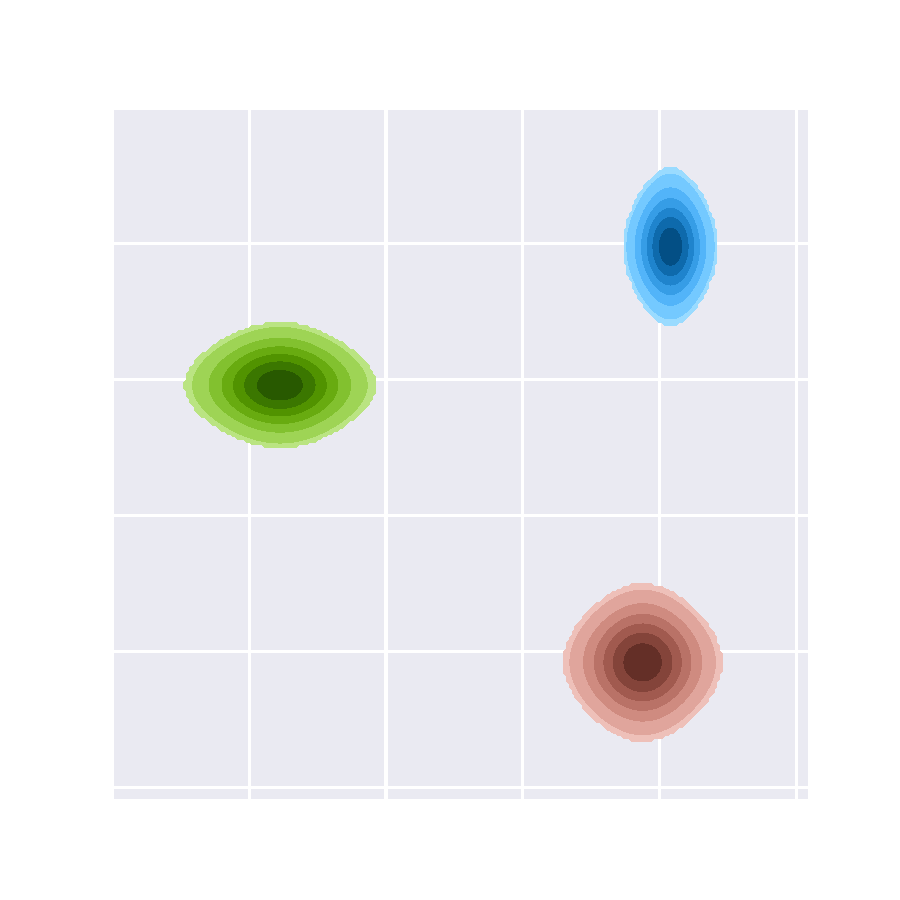
\includegraphics[width=0.28\textwidth]{figures/appendix_figures/encoding_dist_mixture_pure.pdf} & 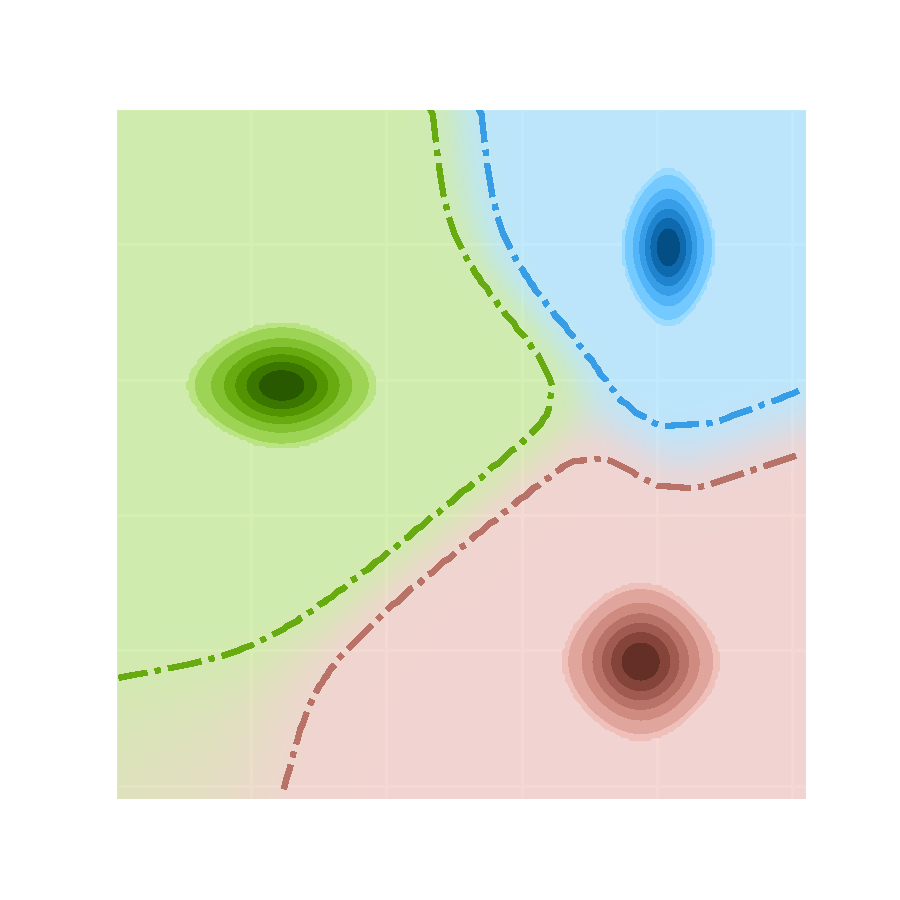
\includegraphics[width=0.28\textwidth]{figures/appendix_figures/encoding_dist_mixture.pdf} \\[3.5mm]
        (a) Encoding distribution $q(\bm{z}_i|x_i)$ & (b) Posterior partitioning $p(x_i|\bm{z_i})$ \\
    \end{tabular}
    \caption[Mixture model encoding]{Visualization of the mixture model encoding and decoding for 3 categories. Best viewed in color. (a) Each category is represented by a logistic distribution with independent mean and scale which are learned during training. (b) The posterior partitions the latent space which is visualized by the background color. The borders show from when on we have an almost unique decoding of the corresponding mixture ($>0.95$ decoding probability). Note that these borders do not directly correspond to the euclidean distance as we use logistic distributions instead of Gaussians.}
    \label{fig:methodology_encoding_dist_mixt}
\end{figure}

Besides a logistic distribution, any other continuous distributions with support over $\mathbb{R}^{d}$ such as Gaussian can also be used for $g(\bm{z}_i)$.
Still, our selection of taking a logistic is based on suitable designs of the continuous normalizing flow $p_{\text{model}}(\bm{z})$, in particular the logistic mixture coupling layer \cite{Flow++} (see Section~\ref{sec:background_comparing_coupling_layers} for a review on this flow layer). 
The logistic mixture layer maps $K$ logistics back into a single mode.
This is particularly useful in Categorical Normalizing Flows if the encoding distribution is a mixture of logistics as the goal of the continuous flow is to map this mixture back to the base distribution which again is a logistic distribution.
Furthermore, it can be shown that for a one-layer autoregressive flow with as many mixtures as the number of categories in the discrete distribution, the likelihood objective falls back to the one of a standard recurrent neural network. 
The proof is detailed in Appendix~\ref{sec:appendix_mixture_optimality}.
This statement implies that an autoregressive Categorical Normalizing Flow can be at least as powerful as an RNN with the same neural network, which has not been the case in previous work \cite{SemiDiscreteNFSequence}.  
Also for non-autoregressive flows, logistic mixture layers provide a strong framework as fewer transformations are needed to accurately model the continuous input distribution. 

\paragraph{Linear flows} Representing each category by a simple logistic distribution considerably limits the encoder's flexibility. 
This flexibility can be increased by applying normalizing flows on each mixture that dependent on the discrete category. 
We refer to this approach as \textit{linear flows} as the flows are applied for each categorical input variable independently.
Formally, we can write the distribution as: 
\begin{eqnarray}
    q(\bm{z}|\bm{x}) & = & \prod_{i=1}^{N} q(\bm{z}_i|x_i)\\
    q\left(\bm{z}^{(K)}\big\vert x_i\right) & = & g\left(\bm{z}^{(0)}\right) \cdot \prod_{k=1}^{K} \left|\det \frac{\partial f_k(\bm{z}^{(k-1)}; x_i)}{\partial \bm{z}^{(k-1)}}\right|\hspace{2mm}\text{where}\hspace{2mm}\bm{z}_i=\bm{z}^{(K)}
\end{eqnarray}
where $f_1,...,f_K$ are invertible, smooth transformations and $g$ represents a logistic distribution with $\mu=0, \sigma=1$. 
In particular, we use here a sequence of coupling layers with activation normalization and invertible 1x1 convolutions \cite{Glow}. 
Both the activation normalization and coupling use the category $x_i$ as an additional external input to determine their transformation parameters by a neural network. 
The class-conditional transformations could also be implemented by storing $K$ parameter sets for the coupling layer neural networks, which is however inefficient for a larger number of categories.  
An example of possible encoding distributions with linear flows is visualized in Figure~\ref{fig:methodology_encoding_dist_linear_flows}. 

\begin{figure}[t!]
    \centering
    \setlength{\tabcolsep}{20pt}
    \begin{tabular}{cc}
        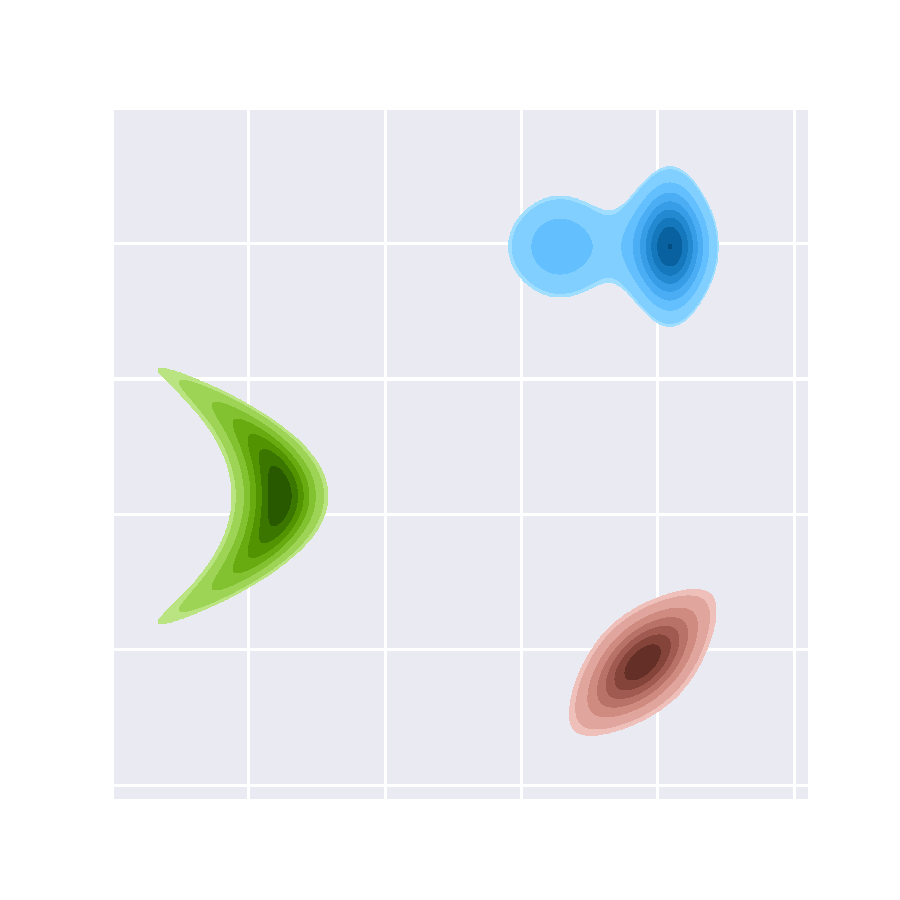
\includegraphics[width=0.28\textwidth]{figures/appendix_figures/encoding_dist_linear_flows_pure.pdf} & 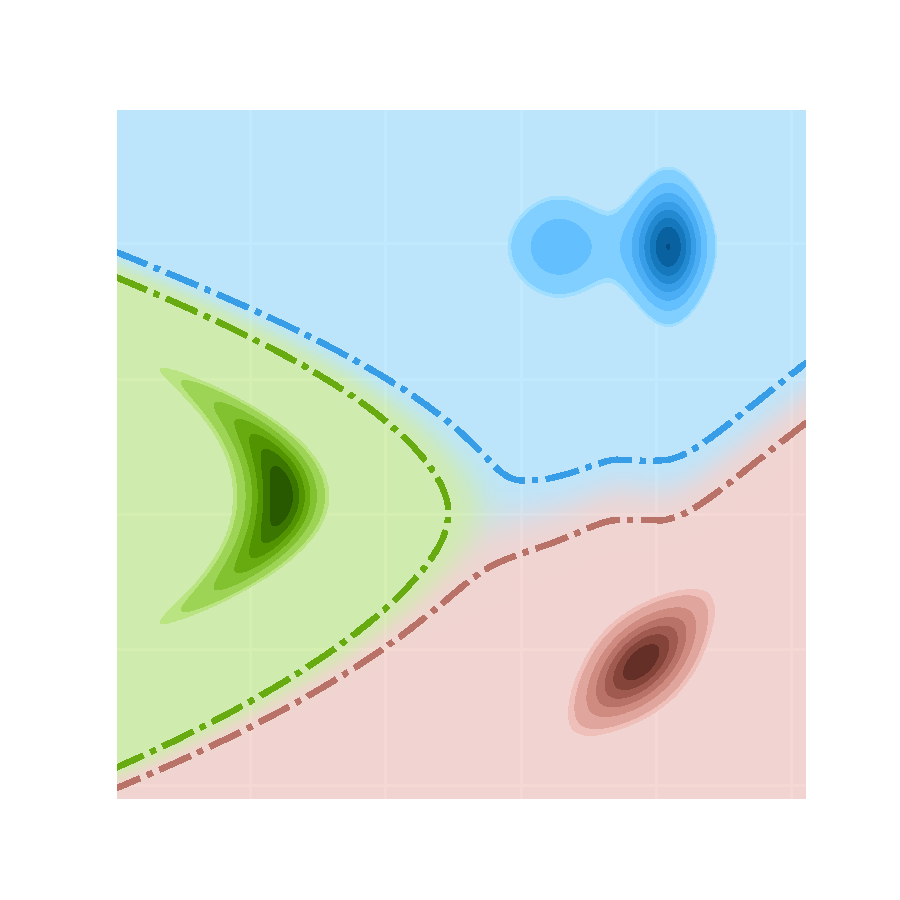
\includegraphics[width=0.28\textwidth]{figures/appendix_figures/encoding_dist_linear_flows.pdf} \\[3.5mm]
        (a) Encoding distribution $q(\bm{z}_i|x_i)$ & (b) Posterior partitioning $p(x_i|\bm{z_i})$ \\
    \end{tabular}
    \caption[Linear flow encoding]{Visualization of the linear flow encoding and decoding for 3 categories. Best viewed in color. (a) The distribution per category is not restricted to a simple logistic and can be multi-modal, rotated or transformed even more. (b) The posterior partitions the latent space which is visualized by the background color. The borders show from when on we have an almost unique decoding of the corresponding category distribution ($>0.95$ decoding probability). Those borders can take any form due to the posteriors flexibility.}
    \label{fig:methodology_encoding_dist_linear_flows}
\end{figure}

Similarly to the mixture model, we can calculate the true posterior $p(x_i|\bm{z}_i)$ using Bayes rule. 
Thereby, we sample from the flow for $x_i$ and need to invert the flows for all other categories. 
Note that as the inverse of the flow also needs to be differentiable by stochastic gradient descend in this situation, we apply affine coupling layers instead of logistic mixture layers.
However, executing linear flows for every categorical variable becomes computationally expensive when there exist more than 20 categories, and thus we use a single-layer linear network as posterior in these cases.


\paragraph{Variational encoding}
The third encoding distribution we experimented with is inspired by variational dequantization \cite{Flow++} and models $q(\bm{z}|\bm{x})$ by one flow across all categorical variables.
With this setup, the encoder distribution can model dependencies across categorical variables and allows even more complex representations than linear flows.
Nevertheless, the posterior, $p(x_i|\bm{z}_i)$, is still applied for each categorical variable independently to maintain the unique decoding and partitioning of the latent space. 
Thus, although the distribution for a category depends on the entire input $\bm{x}$ and the continuous representation of the other variables, all representations of this category are limited to their part in the latent space.
For instance, the category $a$ in the input $\bm{x}=[a,b]$ can be differently represented than in the input $\bm{x}=[a,c]$, but both distribution lie in the same partition modeled by the posterior. 
As the true posterior cannot be found for this distribution, we apply a small linear network to determine $p(x_i|\bm{z}_i)$. 


\subsection{Graph generation with Categorical Normalizing Flows}
\label{sec:methodology_GraphCNF}
Categorical Normalizing Flows can be applied to any task involving categorical data, of which one is graph modeling.
A graph $\mathcal{G}=(V,E)$ is defined by a set of nodes $V$ and a set of edges $E$ whose elements can have attributes that are often categorical. 
When modeling a graph, both the attributes and the overall graph structure need to be considered.
The most successful current approaches \cite{GraphRNNAttention, MolecularRNN, GraphAF, GraphRNN} are autoregressive although graphs are usually not sequential data. \citet{OrderMatters} has shown that treating set-like data as a sequence can significantly hurt performance, and we validate this issue in experiments on graph coloring in Section~\ref{sec:experiments_graph_coloring}. 
Furthermore, a likelihood-based model should intuitively assign equal probability to any permutation or order of the nodes as all of them represent the same graph.

Starting from Categorical Normalizing Flows, we propose GraphCNF, a normalizing flow for graph generation that is invariant to the order of nodes by generating all nodes and edges at once.
Given a graph $\mathcal{G}$, we model each node and edge as a separate categorical variable where the categories correspond to their discrete attributes. 
However, we also need to model whether there exists an edge between two nodes at all or not, as this changes across graphs. 
We implement this by adding an extra category to the edges representing the missing or \textit{virtual} edges. 
Hence, to model an arbitrary graph, we consider an edge variable for every possible tuple of nodes.
To apply normalizing flows on the node and edge categorical variables, we map them into continuous latent space using Categorical Normalizing Flows. 
Subsequent coupling layers map those representations to a continuous prior distribution.
Thereby, GraphCNF uses two crucial design choices for graph modeling: (1) we perform the generation stepwise for improved efficiency, and (2) we ensure that the model assigns an equal likelihood to any ordering of the nodes.

\begin{figure}[t!]
	\centering
	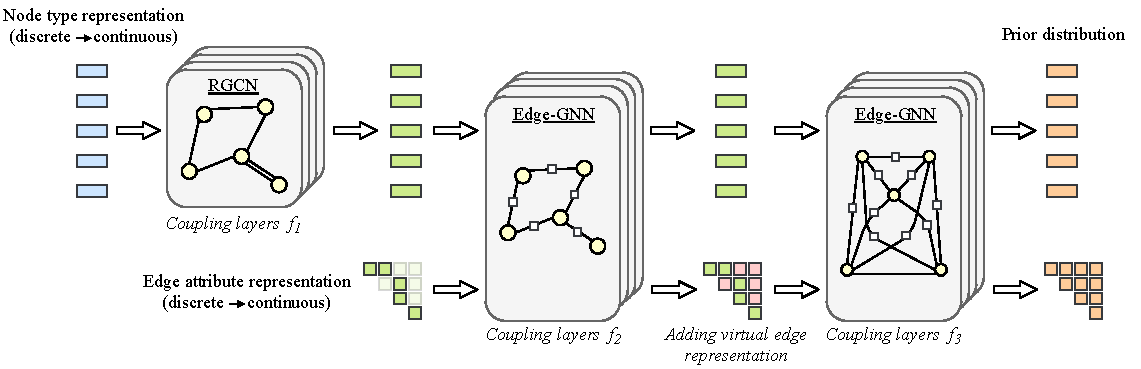
\includegraphics[width=\textwidth]{figures/methodology_figures/GraphCNF.pdf}
	\caption[Model architecture of GraphCNF]{Visualization of GraphCNF for an example graph of five nodes. We add the node and edge attributes, as well as the virtual edges stepwise to the latent space while leveraging the graph structure in the coupling layers. The last step considers a fully connected graph with features per edge.
	}
	\label{fig:methodology_graph_flow}
\end{figure}

\subsubsection{Three-step generation}
Modeling all edges including the virtual ones requires a significant amount of latent variables and is computationally expensive.
However, normalizing flows have been shown to benefit from splitting of latent variables at earlier layers while increasing efficiency \cite{RealNVP, Glow}. 
Furthermore, generating nodes based on the graph structure is a significantly easier task than jointly modeling the nodes with the edges as previous work has shown \cite{GraphNVP}.
Thus, we propose to add the node types, edge attributes, and graph structure stepwise to the latent space as visualized in Figure~\ref{fig:methodology_graph_flow}. 

In the first step, we encode the nodes into continuous latent space, $\bm{z}_0^{(V)}$, using Categorical Normalizing Flows. On those, we apply a group of coupling layers, $f_1$, which additionally use the adjacency matrix and the edge attributes, denoted by $E_{attr}$, as input. Thus, we can summarize the first step as:
\begin{eqnarray}
    z_{1}^{(V)} & = & f_1\big(z_{0}^{(V)}; E, E_{attr}\big)
\end{eqnarray}
The second step incorporates the edge attributes, $E_{attr}$, into latent space. Hence, all edges of the graph except the virtual edges are encoded into latent variables, $\bm{z}_0^{(E_{attr})}$, representing their attribute. The following coupling layers, denoted by $f_2$, transform both the node and edge attribute variables:
\begin{eqnarray}
    z_{2}^{(V)}, z_{1}^{(E_{attr})} & = & f_2\big(z_{1}^{(V)}, z_{0}^{(E_{attr})}; E\big)
\end{eqnarray}
Finally, we add the virtual edges to the latent variable model as $z_{0}^{(E^*)}$. Thereby, we need to slightly adjust our encoding from Categorical Normalizing Flows as we considered the virtual edges as an additional category of the edges. 
While the other categories are already encoded by $\bm{z}_{1}^{(E_{attr})}$, we add a separate encoding distribution for the virtual edges.
This distribution is modeled by a logistic base distribution with one additional flow layer (affine coupling, activation normalization, and invertible 1x1 convolution).
Meanwhile, the decoder needs to be applied on all edges, as we have to distinguish the continuous representation between virtual and non-virtual edges. 
Overall, the mapping can be summarized as:
\begin{eqnarray}
    z_{3}^{(V)}, z_{1}^{(E)} & = & f_3\big(z_{2}^{(V)}, z_{0}^{(E)}\big)\hspace{3mm}\text{where}\hspace{3mm}z_{0}^{(E)} = \big[z_{1}^{(E_{attr})}, z_{0}^{(E^*)}\big]
\end{eqnarray}
where the latent variables $z_{3}^{(V)}$ and $z_{1}^{(E)}$ are trained to follow a prior distribution. 
During sampling, we first invert $f_3$ and determine the general graph structure. Next, we invert $f_2$ and reconstruct the edge attributes. Finally, we apply the inverse of $f_1$ and determine the node types. 

\subsubsection{Permutation-invariant graph modeling}
To make sure that the transformations of the coupling layers are permutation invariant,
we apply a channel masking strategy \cite{RealNVP} such that the split between latent variables is independent of the order of the nodes.
Specifically, the split is performed over the latent dimensions for each node and edge independently.
Secondly, we leverage the graph structure in the coupling networks by applying graph neural networks. 
In the first step, $f_1$, we use a Relation GCN \cite{RGCN} which incorporates the categorical edge attributes into the layer.
For the second and third step, we need a graph network that supports the modeling of both node and edge features.
We refer to this network as Edge-GNN, and we found that various implementations work well.
The specific layer we used is described in the next paragraph.
Using both design choices, GraphCNF assigns equal probability to any ordering of nodes in a graph.

\paragraph{Edge-GNN} GraphCNF implements a three-step generation approach, for which the second and third step also models latent variables for edges. Hence, in the coupling layers, we need a graph neural network which supports both node and edge features. We implement this by alternating between updates of the edge and the node features. Specifically, given node features $\bm{v}^{t}$ and edge features $\bm{e}^{t}$ at layer $t$, we update those as follows:
\begin{eqnarray}
    \bm{v}^{t+1} & = & f_{node}(\bm{v}^{t}; \bm{e}^{t})\\
    \bm{e}^{t+1} & = & f_{edge}(\bm{e}^{t}; \bm{v}^{t+1})
\end{eqnarray}
The update functions, $f_{node}$ and $f_{edge}$, are both common graph neural network layers with slight adjustments to allow a communication between nodes and edges. 
Before detailing the update layers, it should be noted that we use Highway GNNs \cite{HighwayGNN} which apply a gating mechanism. 
Specifically, the updates for the nodes are determined by:
\begin{eqnarray}
    \bm{v}^{t+1} & = & \bm{v}^{t} \cdot T\left(\tilde{\bm{v}}^{t+1}\right) + H\left(\tilde{\bm{v}}^{t+1}\right) \cdot \left(1 - T\left(\tilde{\bm{v}}^{t+1}\right)\right)
\end{eqnarray}
where $\tilde{\bm{v}}^{t+1}$ is the output of the GNN layer. 
$H$ and $T$ represent single linear layer networks where $T$ has a consecutive sigmoid activation to limit the outputs between 0 and 1. 
The edge updates are applied similarly. 
We experienced that such a gated update function helps the gradient flow through the layers back to the input. 
This is important for normalizing flows as coupling layers or transformations in general strongly depend on previous transformations. 
Hence, we apply the same gating mechanism in the first step of GraphCNF, $f_1$.

\begin{figure}[t!]
    \centering
    \begin{subfigure}{.3\textwidth}
        \centering
        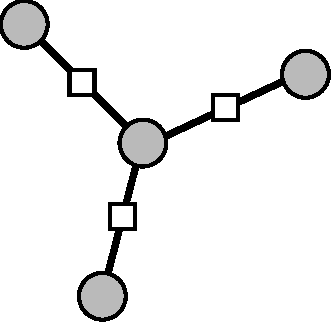
\includegraphics[height=3.5cm]{figures/methodology_figures/EdgeGNN/example_graph.pdf}
        \caption{Example graph}
        \label{fig:methodology_edgeGNN_example_graph}
    \end{subfigure}
    \hfill
    \begin{subfigure}{.3\textwidth}
        \centering
        \vfill
        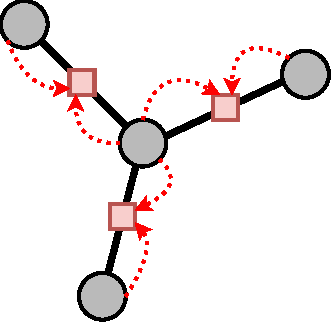
\includegraphics[height=3.5cm]{figures/methodology_figures/EdgeGNN/edge_update.pdf}
        \caption{Edge update $f_{edge}$}
        \label{fig:methodology_edgeGNN_edge_update}
    \end{subfigure}
    \hfill
    \begin{subfigure}{.3\textwidth}
        \centering
        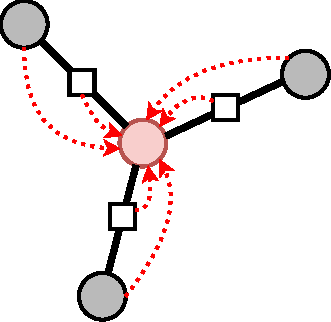
\includegraphics[height=3.5cm]{figures/methodology_figures/EdgeGNN/node_update.pdf}
        \caption{Node update $f_{node}$}
        \label{fig:methodology_edgeGNN_node_update}
    \end{subfigure}
    \caption[Edge and node udpates in EdgeGNN]{
    High-level visualization of the feature updates in EdgeGNN on an example graph (a). (b) The edge features are updated by taking into account the adjacent nodes. (c) For the node features, both the features of the neighbouring nodes as well as its edges are taken into consideration. For readability, only the update of the center node is shown although the features of all nodes are updated in parallel.}
    \label{fig:methodology_edgeGNN}
\end{figure}

Next, we detail the GNN layers to obtain $\tilde{\bm{e}}^{t+1}$ and $\tilde{\bm{v}}^{t+1}$. 
A visualization of the interaction between edge and node features in the updates is shown in Figure~\ref{fig:methodology_edgeGNN}.
The edge update layer $f_{edge}$ resembles a graph convolutional layer \cite{GraphOverview1}, and can be specified as follows:
\begin{equation}
	\tilde{e}^{t+1}_{ij} = g\left({W}^{t}_e e^{t}_{ij} + {W}^{t}_v v^{t}_{i} + {W}^{t}_v v^{t}_{j}\right)
\end{equation}
where $e^{\cdot}_{ij}$ represents the features of the edge between node $i$ and $j$. 
$g$ denotes the GELU \cite{GELU} non-linear activation function. 
In our experiments, using more complex transformations for the edge update layer did not give any notable improvements on the performance of GraphCNF.

To update the node representations, we took inspiration from the transformer architecture \cite{AttentionIsAllYouNeed} and use a modified multi-head attention layer on graphs. 
In particular, a linear transformation maps each node to a key, query and value vector:
\begin{eqnarray}
	K_{v_{i}}, Q_{v_{i}}, V_{v_{i}} & = & W_K v^{t}_{i}, W_Q v^{t}_{i}, W_V v^{t}_{i}
\end{eqnarray}
The attention value is usually computed based on the dot product between two nodes. 
However, as we explicitly have features for the edge between the two nodes, we use those to control the attention mechanism. 
Hence, we have an additional weight matrix $u$ to map the edge features to an attention bias:
\begin{eqnarray}
	\hat{a}_{ij} & = & Q_{v_{i}}K^T_{v_{i}}/\sqrt{d} + e^{t+1}_{ij}u^T
\end{eqnarray}
where $d$ represents the hidden dimensionality of the features. 
Finally, we also add an edge-based value vector to allow full communication from edges to nodes. 
Overall, the updates of the node features are calculated by:
\begin{eqnarray}
	a_{ij} & = & \frac{\exp\left(\hat{a}_{ij}\right)}{\sum_{m}\exp\left(\hat{a}_{im}\right)}, \\
	\tilde{v}^{t+1}_{i} & = & \sum_{j} a_{ij}\cdot \left[V_{v_{j}} + W_e  e^{t+1}_{ij}\right]
\end{eqnarray}
Alternatively to transformers, we also experimented with Graph Attention Networks \cite{GraphAttentionNetwork}. 
However, those showed slightly worse results which is why we used the transformer-based layer for the experiments in this thesis.

In step 2, the (binary) adjacency matrix is given such that each node has a limited number of neighbors. 
A full transformer-based architecture as above is then not necessary anymore as every node has usually a small set of neighbors (e.g. up to 5). 
% In this case, the node-to-node dot product is expensive to perform. 
Hence, we experimented with a node update layer where the attention is purely based on the edge features in step 2. 
We found both to work equally well while the second is computationally more efficient.

\subsubsection{Encoding graph size}
The number of nodes $N$ varies across graphs in the dataset, and hence a generative model needs to be flexible regarding $N$. 
To encode the number of nodes, we use a similar approach as \citet{SemiDiscreteNFSequence} for sequences and add a simple prior over $N$. 
The prior is parameterized based on the graph size frequency in the training set.
Alternatively, to integrate the number of nodes in the latent space, we could add \textit{virtual} nodes to the model, similar to virtual edges. 
Every graph in the training dataset would be filled up to the maximum number of nodes by adding such virtual nodes. 
Meanwhile, during sampling, we remove virtual nodes if the model generates such. 
GraphNVP \cite{GraphNVP} uses such an encoding as their coupling layers did not support flexible graph sizes. 
However, in experiments, we obtained similar performance with both size encodings while the external prior is computationally more efficient and therefore used in this work.
\newpage
\section{Experiments}
\label{sec:experiments}

To show the wide applicability of Categorical Normalizing Flows, we perform experiments on sets, graphs, and language modeling. 
Our goal is to investigate whether Categorical Normalizing Flows can accurately model categorical distributions despite modeling a lower bound, and what flexibility of the encoding distributions is needed for that.
Furthermore, we compare our method to baselines such as Discrete Normalizing Flows \cite{TranDiscreteFlows} and variational dequantization \cite{Flow++}. 

We study the application of Categorical Normalizing Flows on graphs on two tasks: graph coloring and molecule generation. 
On graph coloring, we examine the effect of different node orderings in autoregressive models and compare their performance to the permutation-invariant GraphCNF.
Meanwhile, molecule generation resembles a complex modeling task with various categorical node and edge attributes.
Also, there has been recent work on applying normalizing flows on molecule generation which serve as a comparison to GraphCNF and show the effect of our architectural design choices \cite{GraphNVP, GraphAF}.
A final discussion of the findings in all experiments and an additional analysis is provided in Section~\ref{sec:experiments_discussion}.

The normalizing flows we use in our experiments consist of a sequence of logistic mixture coupling layers proposed by \citet{Flow++} which map a mixture of logistic distributions back into a single mode. 
As mentioned before, this is particularly of interest for our proposed encoding strategy as its simplest implementation is based on a logistic mixture model.
Before each coupling layer, we follow current standard techniques and include an activation normalization layer and invertible 1x1 convolution \cite{Glow}.  
For full reproducibility, we outline each experiment's hyperparameter details in Appendix~\ref{sec:appendix_hyperparams}, and publish our code\footnote{Our code can be found at \href{https://github.com/phlippe/CategoricalNF}{https://github.com/phlippe/CategoricalNF}}.

\begin{figure}[ht!]
    \centering
    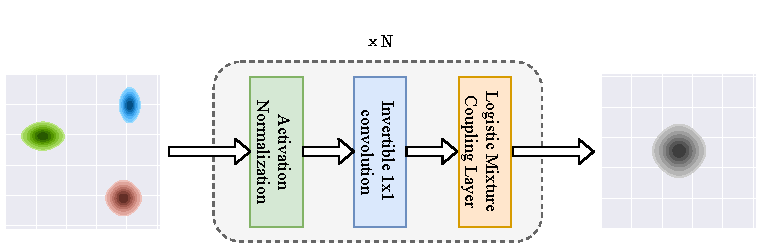
\includegraphics[width=0.75\textwidth]{figures/experiments_figures/flow_template_overview.pdf}
    \caption[Flow architecture in experiments]{Overview of the general flow architecture used in our experiments. We apply a sequence of activation normalization, invertible 1x1 convolution and logistic mixture coupling layer to map the categorical encoding (left) to a logistic base distribution (right). In case of GraphCNF, we use this sequence of flow layers within the three steps $f_1$, $f_2$ and $f_3$.}
    \label{fig:experiments_flow_template_overview}
\end{figure}


\subsection{Set modeling}
\label{sec:experiments_set_modeling}

\paragraph{Task} Sets have the unique property of being a collection of elements with no specific order. 
In order to evaluate how well different normalizing flows can model categorical distributions on sets, we create two toy datasets with a known data likelihood:  \textit{set shuffling} and \textit{set summation}. 
In set shuffling, we model a set of $N$ categorical variables each having one out of $N$ categories. 
However, each category has to appear exactly once in the set. 
Taking for instance $N=4$, we consider the set $\{1,2,3,4\}$.
Although the dataset consists of a single set, this set represents $N!$ possible assignments that need to be modeled. 
For the second toy dataset, set summation, we again consider a set of size $N$ with $N$ categories, but those categories represent the actual integers $1,2,...,N$. 
The task is to model those sets for which the sum of all elements is an arbitrary number, $L$. 
In contrast to the shuffling dataset, the data is ordinal in set summation, which we initially expected to help dequantization methods. 
In our experiments, we used $N=16$ for both datasets and $L=42$ for the summing dataset which gave us about 2000 different sets in the dataset.
For both datasets, we can compute the true likelihood in bits per element by determining the number of possible permutations for all instances together, denoted by $M$, and dividing its overall log-likelihood by the sequence length: $(\log_2 M)/N$. 

\paragraph{Models} We compare Categorical Normalizing Flows to applying variational dequantization \cite{Flow++}, Latent Normalizing Flows \cite{SemiDiscreteNFSequence} and Discrete Normalizing Flows by \citet{TranDiscreteFlows} with a factorized prior. 
In Categorical Normalizing Flows, we use a latent dimensionality of $d=4$ for each categorical variable and apply a channel mask making the flow permutation-invariant to its inputs.
While Latent Normalizing Flows can follow this setup as well, variational dequantization and Discrete NFs have to use a checkboard mask, i.e. masking every other element of the sequence, since they rely on a single dimension per discrete variable. Thus, these flows are sensitive to the order in the set.
For a fair comparison, all flows use the same setup of 8 coupling layers with a 2-layer transformer \cite{AttentionIsAllYouNeed} excluding the positional encoding. 
% We explicitly do not use positional encoding as commonly applied in transformers to maintain the permutation invariance of the data. 
Besides, we vary the encoding distribution in Categorical Normalizing Flows and compare a mixture model, linear flows, and variational encoding.
The Latent Normalizing Flows use a 2-layer transformer to determine the mean and scale of the logistic encoding distribution, and a second transformer network as decoder.

\begin{table}[t!]
	\caption[Results on set modeling]{Results on set modeling. Metric used is bits per categorical variable (dimension). The standard deviation across three seeds is reported next to the average of the models.}
	\label{tab:result_table_sets}
	\centering
	\begin{tabular}{lccc}
		\toprule
		\textbf{Model} & \textbf{Set shuffling} & \textbf{Set summation} \\
		\midrule
		Discrete NF \cite{TranDiscreteFlows} & $3.87$ \footnotesize{$\pm0.04$} & $2.51$ \footnotesize{$\pm0.00$}\\
		Variational Dequant. \cite{Flow++} & $3.01$ \footnotesize{$\pm0.02$} & $2.29$ \footnotesize{$\pm0.01$}\\
		Latent NF \cite{SemiDiscreteNFSequence} & $\bm{2.78}$  \footnotesize{$\pm0.00$} & $2.26$ \footnotesize{$\pm0.01$}\\[4pt]
		CNF $+$ Mixture model & $\bm{2.78}$ \footnotesize{$\pm0.00$} & $\bm{2.24}$  \footnotesize{$\pm0.00$}\\
		CNF $+$ Linear flows & $\bm{2.78}$ \footnotesize{$\pm0.00$} & $2.25$ \footnotesize{$\pm0.00$}\\
		CNF $+$ Variational Encoding & $2.79$ \footnotesize{$\pm0.01$} & $2.25$ \footnotesize{$\pm0.01$}\\
		\midrule 
		%Unigram & $4.00$bpd & $2.51$bpd \\
		Optimal & $2.77$ & $2.24$ \\
		\bottomrule
	\end{tabular}
\end{table}

\paragraph{Results} Our results are summarized in Table~\ref{tab:result_table_sets}. 
On both datasets, Categorical Normalizing Flows achieve close-to-optimal performance with a maximum offset of $0.01$bpd. 
This shows that although we model a lower bound in continuous space, Categorical Normalizing Flows can model discrete distributions precisely. 
Interestingly, representing the categories by a simple mixture model is sufficient for achieving these results, and more complex encoding distributions did not result in improvements. 
We observed the same trend in experiments with more complex relations between categories, such as on the graph and language modeling. 
This is presumably because of both the coupling layers and the prior distribution rest upon logistic distributions as well.
Modeling a different encoding distribution would require additional transformations inside the flow to map them back to a logistic base distribution.
This hypothesis is supported when taking a closer look at the distributions learned by linear flows and the variational encoding.
We experienced that both have fallen back to a logistic distribution per category despite being able to model much more complex distributions.
Hence, we can conclude that encoding categorical variables by a simple mixture model is indeed sufficiently powerful and efficient.

Introducing dependencies between categorical variables during decoding, as done in Latent Normalizing Flows, also shows to achieve good performance although slightly lower on set summation.
On set shuffling, the encoding parameters are constant since we only learn a single set such that the input to the encoder is always the same. 
Thus, the model effectively falls back to a mixture model.
To train Latent NFs on set summation, weighting the reconstruction error of the decoder significantly higher than the prior in the beginning of the training showed to be crucial.
In this phase, the decoder learns to be deterministic and the prior is complex enough to model the latent space consecutively.
This weighting is similar to the KL scheduling that is commonly done in VAEs and follow \citet{SemiDiscreteNFSequence} original setup.
Nevertheless, it should be kept in mind that Latent NFs model a lower bound which also attributes to the slightly higher bits per dimension score.

Meanwhile, the variational dequantization obtains a considerably worse performance on the shuffling dataset, underlining that dequantization methods cannot represent categorical data well. 
In set summation, where the categories represented integers, we see a closer score, although it is still performing considerably worse than Categorical Normalizing Flows. 
Discrete Normalizing Flows was not able to model the categorical distributions well in our experiments, mostly due to notable optimization issues we experienced. 
Following the hyperparameter setting of \citet{TranDiscreteFlows}, we experienced that discrete flows got stuck in local optima, and gradients vanished due to approximations of discrete operations. 
In contrast, Categorical Normalizing Flows is not suffering from such gradient issues by modeling the transformations in continuous space.

\subsection{Graph coloring}
\label{sec:experiments_graph_coloring}

\paragraph{Task} Graph coloring is a well-known combinatorial problem which finds use in many applications \cite{bondy1976graph, GraphColoringDL, GraphColoringApplications}. 
Given a graph $\mathcal{G}$, the task is to assign each node one out of $K$ colors. However, two adjacent nodes are not allowed to have the same color. 
Consequently, there are a limited number of valid colorings for each graph. 
Modeling the distribution of these solutions to arbitrary graphs is a challenging task as it has been shown to be NP-complete \cite{bondy1976graph}. 
With this experiment, we aim to verify that assuming an order can have a significant influence on autoregressive graph models and that the permutation-invariant GraphCNF can achieve similar performance to the best autoregressive order.

\paragraph{Dataset} To train models on modeling such a distribution, we generate a dataset of graph colorings by randomly sampling a graph and using an SAT solver 
%\footnote{We have used the following solver from the OR-Tools library in python: \href{https://developers.google.com/optimization/cp/cp_solver}{https://developers.google.com/optimization/cp/cp\_solver}} 
for finding one valid coloring assignment. In our experiments, we focus on the 3-color problem meaning that a graph has to be colored using $K=3$ colors. A detailed description of the dataset generation can be found in Appendix
~\ref{sec:appendix_hyperparams_graph_coloring}. We create two dataset versions, one with graphs of size $10\leq|V|\leq20$ and another with $25\leq|V|\leq50$, to further investigate the effect of complexity as larger graphs are commonly harder to solve. Overall, we use 200k and 450k examples for training and evaluate on a test set with 25k previously unseen graphs. We visualize examples of the datasets in Figure~\ref{fig:experiments_graph_coloring_examples}.

\begin{figure}[b!]
    \centering
    \setlength{\tabcolsep}{20pt}
    \begin{tabular}{cc}
        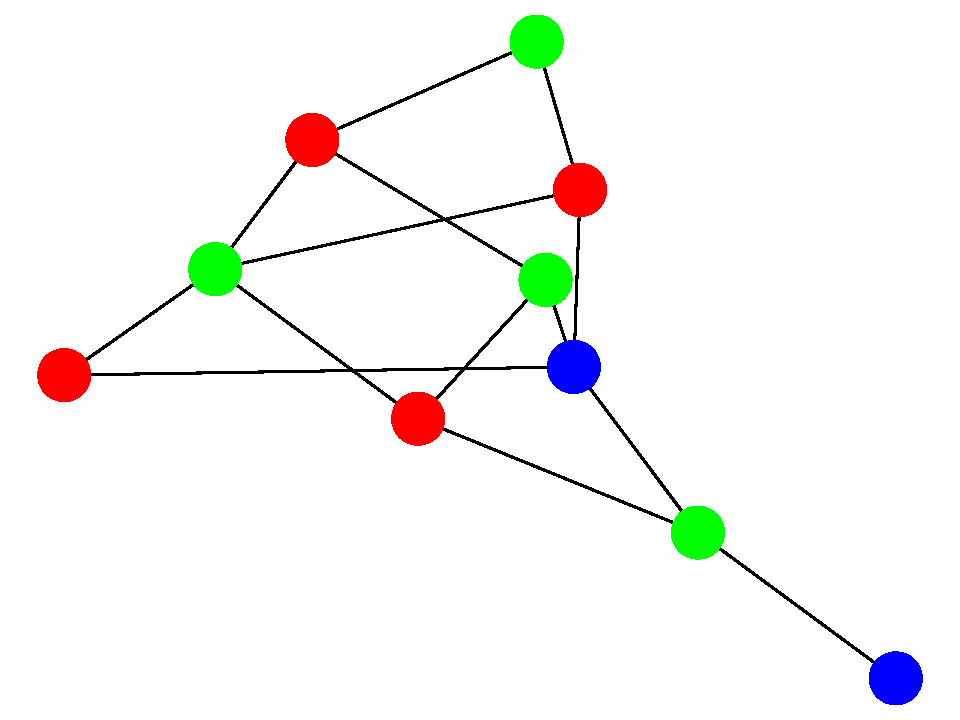
\includegraphics[height=3cm]{figures/experiments_figures/dataset_figures/graph_coloring/exmp_tiny_0.pdf} &  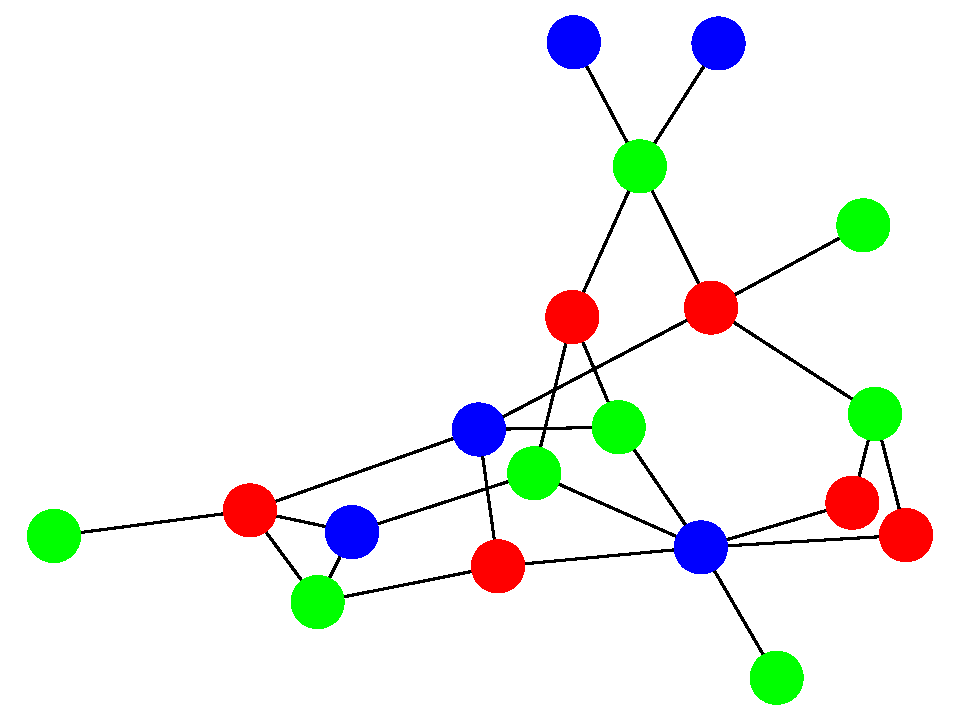
\includegraphics[height=3cm]{figures/experiments_figures/dataset_figures/graph_coloring/exmp_tiny_9.pdf}\\
        (a)  $|V|=10$ & (b)  $|V|=19$\\[4pt]
        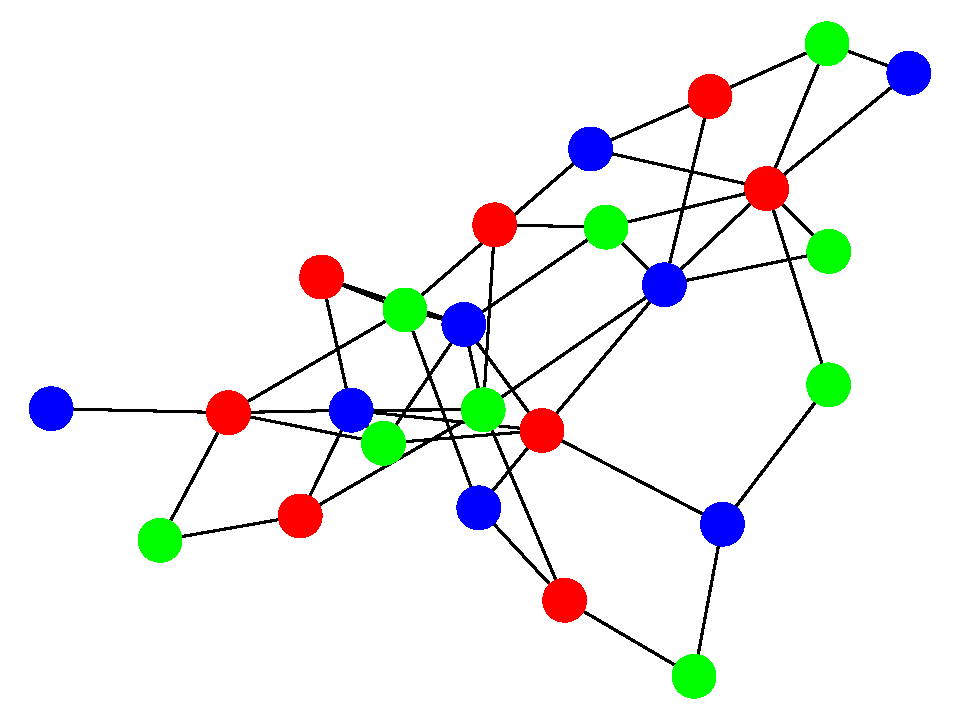
\includegraphics[height=4cm]{figures/experiments_figures/dataset_figures/graph_coloring/exmp_large_4.pdf} & 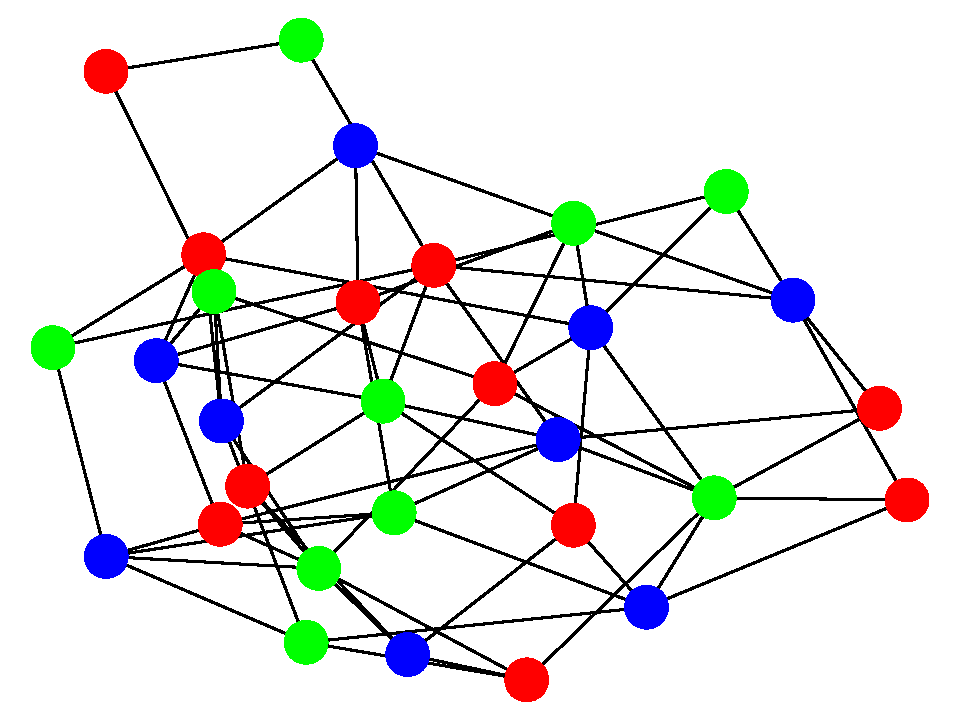
\includegraphics[height=4cm]{figures/experiments_figures/dataset_figures/graph_coloring/exmp_large_9.pdf}\\
        (c)  $|V|=25$ & (d)  $|V|=30$\\
    \end{tabular}
    \caption[Examples of graph coloring]{Examples of valid graph color assignments from the dataset (best viewed in color). Due to the graph sizes and dense adjacency matrices, edges can be occluded or cluttered in (c) and (d).}
    \label{fig:experiments_graph_coloring_examples}
\end{figure}

\paragraph{Models} We compare GraphCNF to a variational autoencoder and an autoregressive prediction model which generates one node at a time. 
Considering graph coloring does not require edge generation, we only use the first step of GraphCNF's three-step generation. 
For all models, we apply the same Graph Attention network \cite{GraphAttentionNetwork}. 
Note that due to the different sampling techniques, we cannot guarantee a fully fair comparison in terms of number of parameters and layer depth across models.
For instance, Normalizing Flows require considerably more parameters than autoregressive models although being much faster to sample from.
Thus, we tried to balance the complexity of the model and the sampling time when designing the models. 
More details can be found in Appendix~\ref{sec:appendix_hyperparams_graph_coloring}.

As autoregressive models require a manually prescribed node order, we compare the following: a \emph{random} ordering per graph, \textit{largest\_first} which is inspired by heuristics of automated theorem provers that start from the nodes with the most connections, and \textit{smallest\_first}, where we reverse the order of the previous heuristic. 

\paragraph{Metrics} We evaluate the models based on two metrics. First, the likelihood of the test dataset is measured by bits per node. A low likelihood shows the generalization property of the model to new graphs, and the coverage of all possible solutions for a graph by the model. 
The second metric we use is \textit{validity}. 
Validity is measured by randomly sampling a color assignment from the model for each graph in the test dataset, and reporting the percentage of samples which were a valid solution by having different colors for all adjacent nodes. 
Therefore, this metric represents the modeled discrete distribution and its closeness to the learned rules. 
Note that we sample with a temperature value of $T=1.0$, meaning that we sample from the original softmax distribution in autoregressive models and the original prior in normalizing flows and variational autoencoders. 
A lower temperature value reduces the variance during sampling and biases the samples towards the most likely values.
Nonetheless, we do not lower it here because we want to test the full discrete distribution of the model.

\begin{table}[t]
	\caption[Results on graph coloring]{Results on the graph coloring problem. The column \textit{time} shows the average time for the different models needed to sample a batch of 128 graph coloring assignments on a NVIDIA TitanRTX. In the last row, we report the results of GraphCNF with affine coupling layers. The standard deviation was omitted for readability and can be found in the appendix, Table~\ref{tab:appendix_results_graph_coloring}.}
	\label{tab:result_table_graph_coloring}
	\centering
	\begin{tabular*}{\columnwidth}{@{\extracolsep{\fill}}l*{6}{c}}
		\toprule
		& \multicolumn{3}{c}{$10\leq|V|\leq20$} & \multicolumn{3}{c}{$25\leq|V|\leq50$} \\
		\cmidrule{2-4} \cmidrule{5-7}
		\textbf{Method} & \textbf{Validity} & \textbf{Bits per node} & \textbf{Time} & \textbf{Validity} & \textbf{Bits per node} & \textbf{Time}  \\
		\midrule
		VAE & $44.95\%$ & $0.84$bpd & $0.05$s & $7.75\%$ & $0.64$bpd & $0.10$s \\
		% Autoregressive & & & $0.69$s & & & $2.88$s \\
		% - Smallest\_first & $76.86\%$ & $0.73$bpd & & $32.27\%$ & $0.50$bpd &\\
		% - Random & $88.62\%$ & $0.70$bpd & & $49.28\%$ & $0.46$bpd &\\
		% - Largest\_first & $93.41\%$ & $0.68$bpd & & $\bm{71.32\%}$ & $\bm{0.43}$bpd &\\
		RNN$+$Smallest\_first & $76.86\%$ & $0.73$bpd & $0.69$s & $32.27\%$ & $0.50$bpd & $2.88$s\\
		RNN$+$Random & $88.62\%$ & $0.70$bpd & $0.69$s & $49.28\%$ & $0.46$bpd & $2.88$s\\
		RNN$+$Largest\_first & $93.41\%$ & $0.68$bpd & $0.69$s & $\bm{71.32\%}$ & $\bm{0.43}$bpd & $2.88$s\\
		\midrule
		GraphCNF & $\bm{94.56\%}$ & $\bm{0.67}$bpd & $0.28$s & $66.80\%$ & $0.45$bpd & $0.54s$\\
		$-$ Affine & $93.90\%$ & $0.69$bpd & $0.12$s & $65.78\%$ & $0.47$bpd & $0.35$s\\
		\bottomrule
	\end{tabular*}
\end{table}

\paragraph{Results} Table~\ref{tab:result_table_graph_coloring} summarizes the results. 
As we initially expected, the node order has a significant effect on the autoregressive model's performance which becomes the clearest in terms of validity. 
While sorting the nodes according to smallest\_first leads to only $32\%$ valid solutions on the large dataset, reversing the order simplifies the task for the model such that it generates more than twice as many valid color assignments. 
The ordering also shows to become more crucial for harder tasks.
In contrast, GraphCNF is invariant of the order of nodes.
Despite generating all nodes in parallel, it outperforms all node orderings on the small dataset, while being close to the largest\_first ordering on the larger dataset. 
Even the bits per node are on par with the autoregressive models.
Although having more parameters, the sampling with GraphCNF is considerably faster than the autoregressive models.
Replacing the logistic mixture coupling layers with standard affine coupling can speed up the sampling in GraphCNF because the mixture coupling requires an iterative algorithm to be inverted.
When using those, the sampling time is about halved while the validity and likelihood slightly suffer. 
This demonstrates that logistic mixture coupling layers are beneficial but not essential for deep Categorical Normalizing Flows.

Interestingly, when finetuning the encoding dimensionality in Categorical Normalizing Flows, we find that while for the small datasets any dimensionality greater than or equals to $2$ obtains good performance, the large dataset considerably benefits from using a higher dimensionality of $6$. 
Given that both datasets use the same number of categories, namely $3$, this difference underlines that a higher dimensionality is not only crucial for encoding, but also for the transformations inside the flow.

In conclusion, the order of nodes has a significant impact on autoregressive models in graph generation tasks. GraphCNF can compete or even outperform autoregressive models with optimized node orderings while being significantly faster in sampling and independent of an order. This is especially beneficial in tasks where an optimal order of nodes is not known, as it is the case for molecule generation. 

\subsection{Molecule generation}
\label{sec:experiments_molecule_generation}

\paragraph{Task} Modeling and generating graphs is a crucial in biology and chemistry for applications such as drug discovery and property optimization, where molecule generation has emerged as a common benchmark \cite{JunctionTreeVAE, GraphNVP, GraphAF}. 
In a molecule graph, the nodes are atoms and the edges represent bonds between atoms, both represented by categorical features. 
Using a dataset of existing molecules, the goal is to learn a distribution of valid molecules as not all possible combinations of atoms and bonds are valid.
For instance, atoms have a limited number of bonds they can form. 
Modeling such a distribution via a latent based model can be useful for applications as drug discovery and property optimization \cite{GraphAF, MolecularRNN}. 

\paragraph{Datasets} We perform experiments on the Zinc250k \cite{Zinc250k} and MOSES \cite{MosesDataset} dataset. 
The Zink250k dataset consists of 250,000 drug-like molecules. The molecules contain up to 38 atoms of 9 different types, with three different bond types possible between the atoms. 
The Moses dataset is significantly larger and contains 1.9 million molecules with up to 30 atoms of 7 different types. 
For both datasets, we follow the preprocessing of \citet{GraphAF} and represent molecules in a form in which hydrogen is removed. 
The distributions of node and edge types are heavily biased in both datasets, as over 70\% of the atoms are carbon, while for instance bromine appears less than 0.002\%. 
This makes the modeling task additionally challenging.

\paragraph{Models} Various approaches have been proposed for molecule generation. 
For baselines to GraphCNF, we focus on models that consider molecules as a graph and not as text representation like SMILES, as we are interested in general graph modeling approaches. 
As VAE-based approaches, we consider R-VAE \cite{GraphVAEConstrained} and Junction-Tree VAE (JT-VAE) \cite{JunctionTreeVAE}. 
R-VAE is a one-shot generation model which uses a regularization framework to ensure semantic validity. 
JT-VAE represents a molecule as a junction tree of sub-graphs that are obtained from the training dataset. 
We also compare our model to GraphNVP \cite{GraphNVP} and GraphAF \cite{GraphAF} as introduced in Section~\ref{sec:related_work_graph_modeling}.

\paragraph{Metrics} The standard evaluation metrics on molecule generation are validity, uniqueness, and novelty, measured on a set of 10,000 samples. Validity describes the proportion of graphs that represent valid molecules. Uniqueness is the percentage of unique graphs, and novelty measures the proportion of generated molecules which have not been seen during training. 
While a high validity shows that the model has learned the rules for creating molecules, a high uniqueness and novelty ensure that the model is not simply memorizing the training dataset or a small set of molecules. 
The fourth metric which is commonly used for VAEs is the proportion of molecules that can be accurately reconstructed from latent space. 
Normalizing flows on the other hand have an invertible mapping and therefore score 100\% on this metric. 
While our encoding does not strictly guarantee a 100\% reconstruction, we test our model on this metric as well to show that it maintains an invertible mapping. 

\paragraph{Results} Table~\ref{tab:result_table_molecule_generation_zinc250k} shows that GraphCNF generates almost twice as many valid molecules than other one-shot approaches. 
Yet, the novelty and uniqueness stay at almost 100\%. 
Even the autoregressive normalizing flow, GraphAF, is outperformed by GraphCNF by 15\%.
However, the rules for generating valid molecules can be enforced in autoregressive models by masking out the invalid outputs. 
This has been the case for JT-VAE as it has been trained with those manual rules, and thus achieves a validity of 100\%. 
Nevertheless, we are mainly interested in the model's capability of learning the rules by itself and being not specific to any application. 
While GraphNVP and GraphAF sample with a lower standard deviation from the prior to increase validity, we explicitly sample from the original prior (temperature $T=1.0$) to underline that our model covers the whole latent space well.

Surprisingly, we found out that most invalid graphs consist of two or more molecules that in isolation are valid. 
This can happen as one-shot generation models have no guidance regarding generating a single connected graph. 
In contrast, autoregressive models do not commonly suffer from this issue as this would require to generate a node without any edges prevented by the manually picked node order.
By taking the largest sub-graph of these predictions, we obtain a validity ratio of $96.35\%$ making our model generate almost solely valid molecules \emph{without any manually encoded rules}. 


\begin{table}[t]
	\caption[Molecule generation results on the Zinc250k dataset]{Performance on molecule generation trained on Zinc250k \cite{Zinc250k}, calculated on 10k samples and averaged over 4 runs. Scores of baselines are taken from their respective papers. % (JT-VAE \cite{JunctionTreeVAE}, GraphAF \cite{GraphAF}, R-VAE \cite{GraphVAEConstrained}, GraphNVP \cite{GraphNVP}). 
	The column \textit{parallel} indicates which model performs one-shot generation (\cmark) and which use autoregressive prediction (\xmark). In the column \textit{general}, (\xmark) denotes that a model is specialized on molecule generation and uses manually encoded rules.
	}
	\label{tab:result_table_molecule_generation_zinc250k}
	\centering
	\begin{tabular}{lcccccc}
        \toprule
        \textbf{Method} & \textbf{Validity} & \textbf{Uniqueness} & \textbf{Novelty} & \textbf{Reconstruction} & \textbf{Parallel} & \textbf{General}\\
        \midrule
        JT-VAE [\citenum{JunctionTreeVAE}] & $100\%$ & $100\%$ & $100\%$ & $71\%$ & \xmark & \xmark\\
        %\footnotesize{\cite{JunctionTreeVAE}} & & & & & \\
        GraphAF [\citenum{GraphAF}] & $68\%$ & $99.10\%$ & $100\%$ & $100\%$ & \xmark & \cmark\\
        %\footnotesize{\cite{GraphAF}} & & & & & \\
        R-VAE [\citenum{GraphVAEConstrained}] & $34.9\%$ & $100\%$ & $-$ & $54.7\%$ & \cmark & \cmark\\
        %\footnotesize{\cite{GraphVAEConstrained}} & & & & & \\
        GraphNVP [\citenum{GraphNVP}] & $42.60\%$ & $94.80\%$ & $100\%$ & $100\%$ & \cmark & \cmark\\
        %\footnotesize{\cite{GraphNVP}} & & & & & \\
        \midrule
        GraphCNF & $83.41\%$  & $99.99\%$ & $100\%$ & $100\%$ & \cmark & \cmark\\
        & \footnotesize{($\pm2.88$)} & \footnotesize{($\pm0.01$)} & \footnotesize{($\pm0.00$)} & \footnotesize{($\pm0.00$)} & & \\[3.5pt]
        $+$ Sub-graphs & $96.35\%$ & $99.98\%$ & $99.98\%$ & $100\%$ & \cmark & \cmark\\
        & \footnotesize{($\pm2.21$)} & \footnotesize{($\pm0.01$)} & \footnotesize{($\pm0.02$)} & \footnotesize{($\pm0.00$)} & &\\
        \bottomrule
    \end{tabular}
\end{table}

\begin{table}[t]
	\caption[Molecule generation results on the Moses dataset]{Performance on Moses \cite{MosesDataset}, calculated on 10k samples and averaged over 4 runs. Score for GraphAF taken from \citet{GraphAF}, and JT-VAE from \citet{MosesDataset}. }
	\label{tab:result_table_molecule_generation_moses}
	\centering
	\begin{tabular}{lcccc}
		\toprule
		\textbf{Method} & \textbf{Validity} & \textbf{Uniqueness} & \textbf{Novelty}\\
		\midrule
		JT-VAE \cite{JunctionTreeVAE} & $100\%$ & $99.92\%$ & $91.53\%$ \\
		GraphAF \cite{GraphAF} & $71\%$\textsuperscript{\dag} & $99.99\%$ & $100\%$ \\
		\midrule
		GraphCNF & $82.56\%$  & $100.0\%$ & $100\%$ \\
		& \footnotesize{($\pm2.34$)} & \footnotesize{($\pm0.00$)} & \footnotesize{($\pm0.00$)} \\[3.5pt]
		$+$ Sub-graphs & $95.66\%$  & $99.98\%$ & $100\%$ & \\
		& \footnotesize{($\pm2.58$)} & \footnotesize{($\pm0.01$)} & \footnotesize{($\pm0.00$)} \\
		\bottomrule
	\end{tabular}
\end{table}

To emphasize that our findings are not limited to a single dataset, we present the results on the Moses dataset in Table~\ref{tab:result_table_molecule_generation_moses}. Overall, our model achieves similar performance on this dataset.
Finally, we show 12 randomly sampled molecules from our model in Figure~\ref{fig:appendix_molecule_generation}. 
In general, GraphCNF can generate a very diverse set of molecules with a variety of atom types, even those that occur less than $0.1\%$ in the dataset. 
This qualitative analysis endorses the previous quantitative results of obtaining close to 100\% uniqueness on 10k samples. 

\begin{figure}[t]
    \centering
    \begin{tabular}{cccc}
        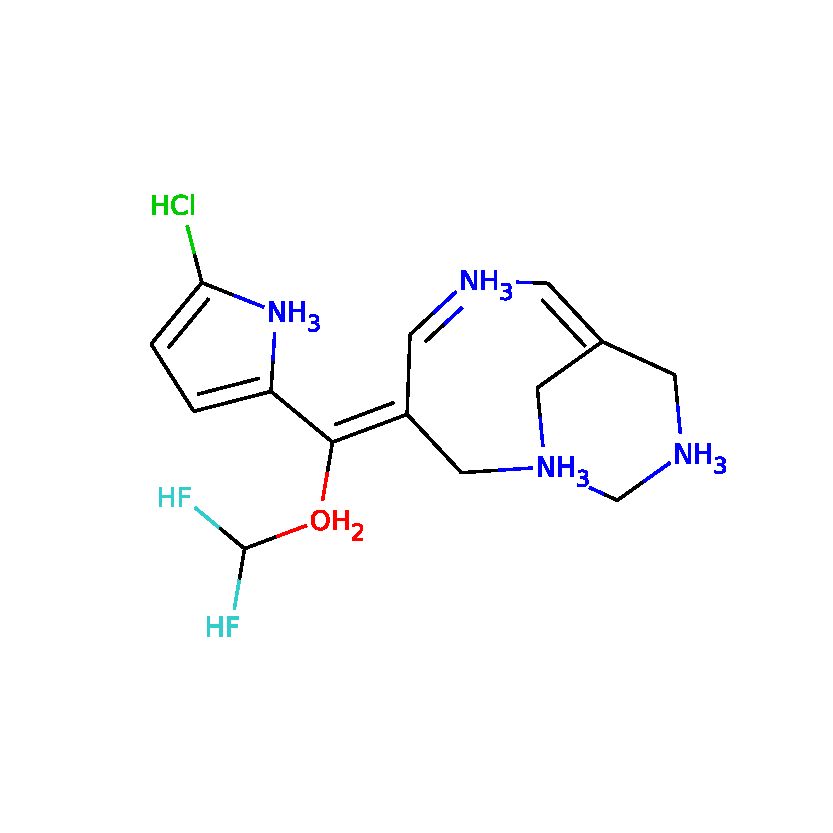
\includegraphics[width=0.22\textwidth]{figures/experiments_figures/molecule_samples/generated_molecule_796_v.pdf} & 
        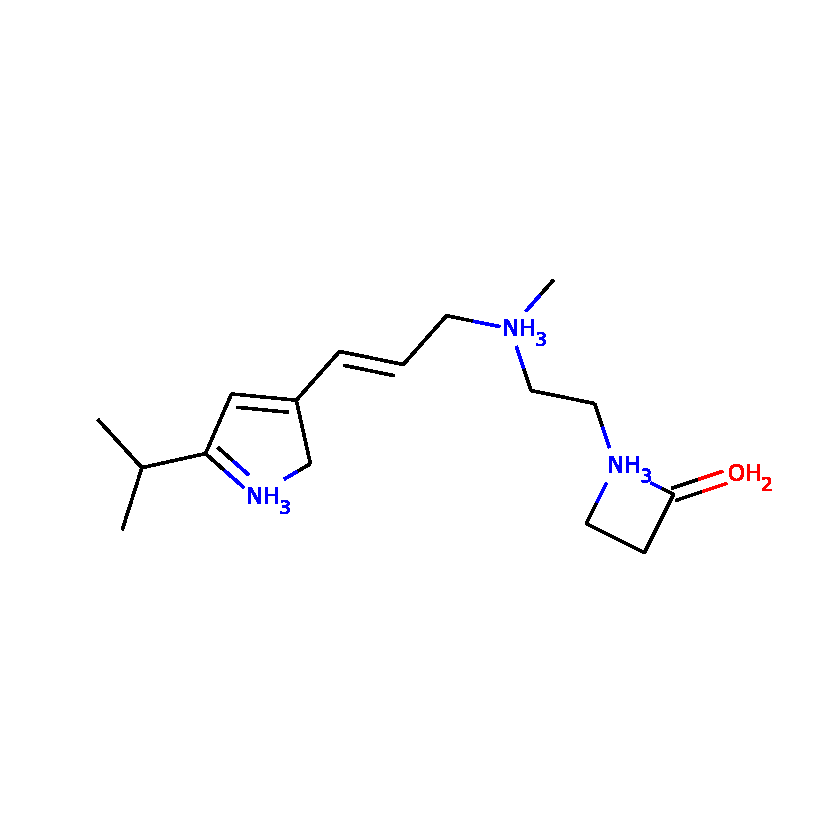
\includegraphics[width=0.22\textwidth]{figures/experiments_figures/molecule_samples/generated_molecule_1_v.pdf}  & 
        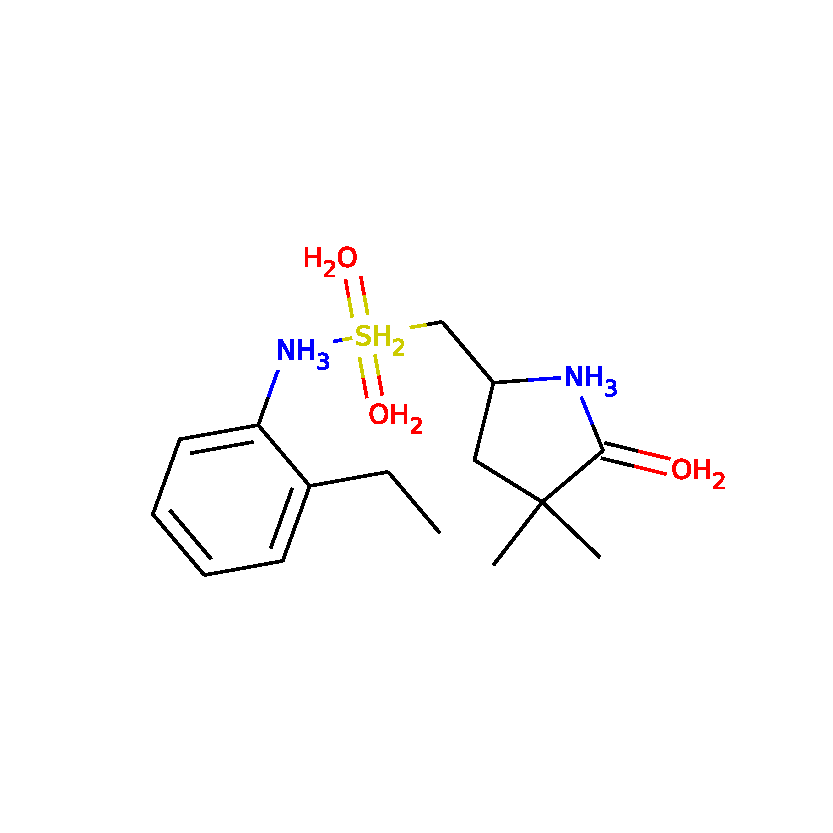
\includegraphics[width=0.22\textwidth]{figures/experiments_figures/molecule_samples/generated_molecule_6_v.pdf}  & 
        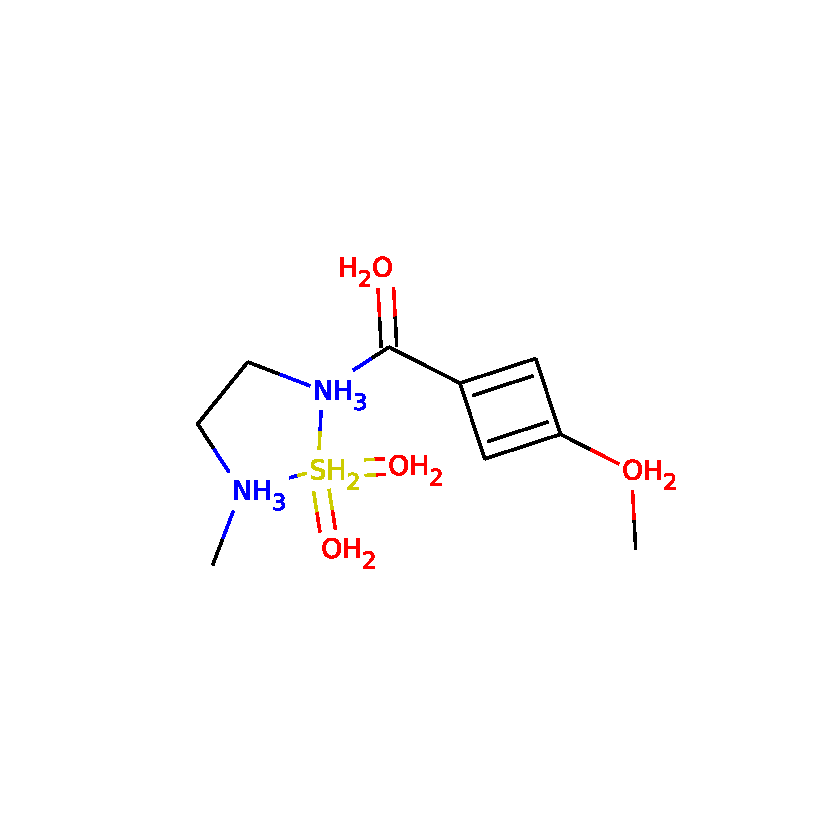
\includegraphics[width=0.22\textwidth]{figures/experiments_figures/molecule_samples/generated_molecule_8_v.pdf} \\ 
        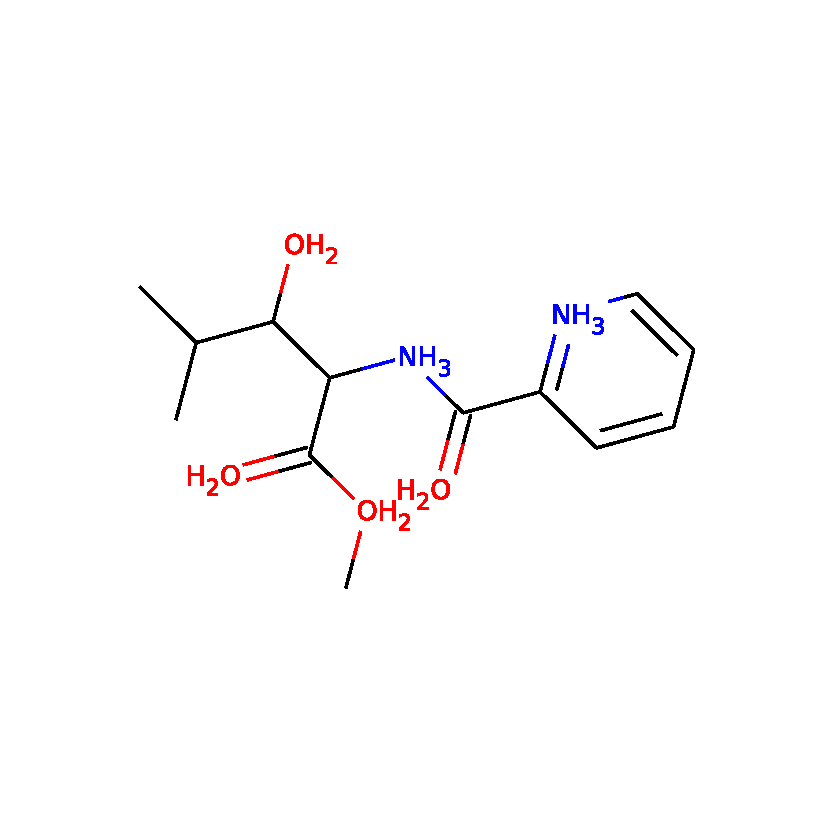
\includegraphics[width=0.22\textwidth]{figures/experiments_figures/molecule_samples/generated_molecule_10_v.pdf} & 
        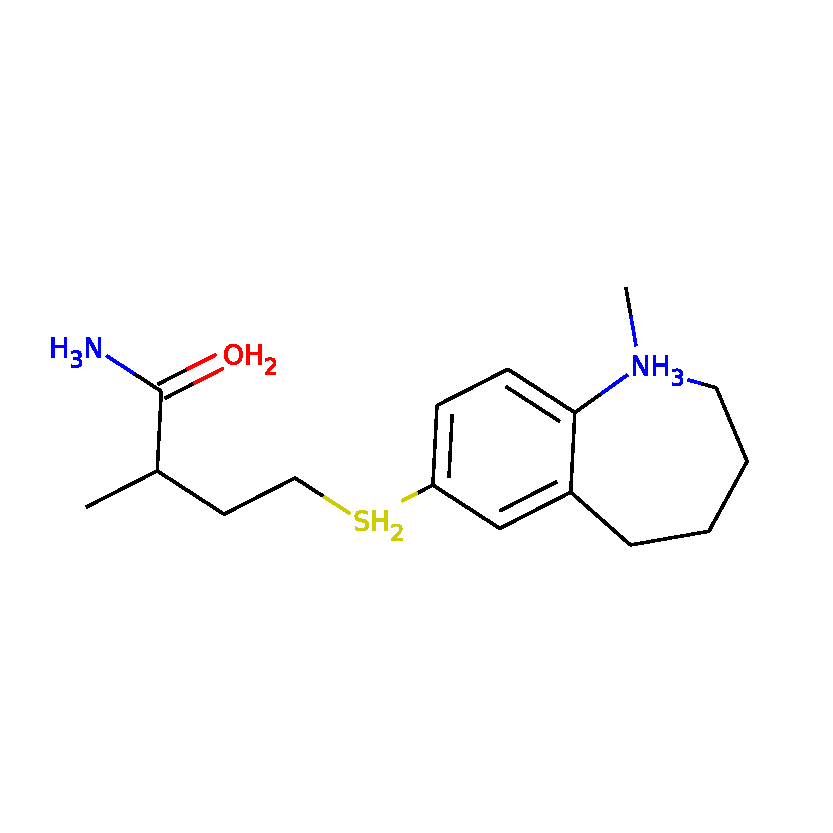
\includegraphics[width=0.22\textwidth]{figures/experiments_figures/molecule_samples/generated_molecule_13_v.pdf} &
        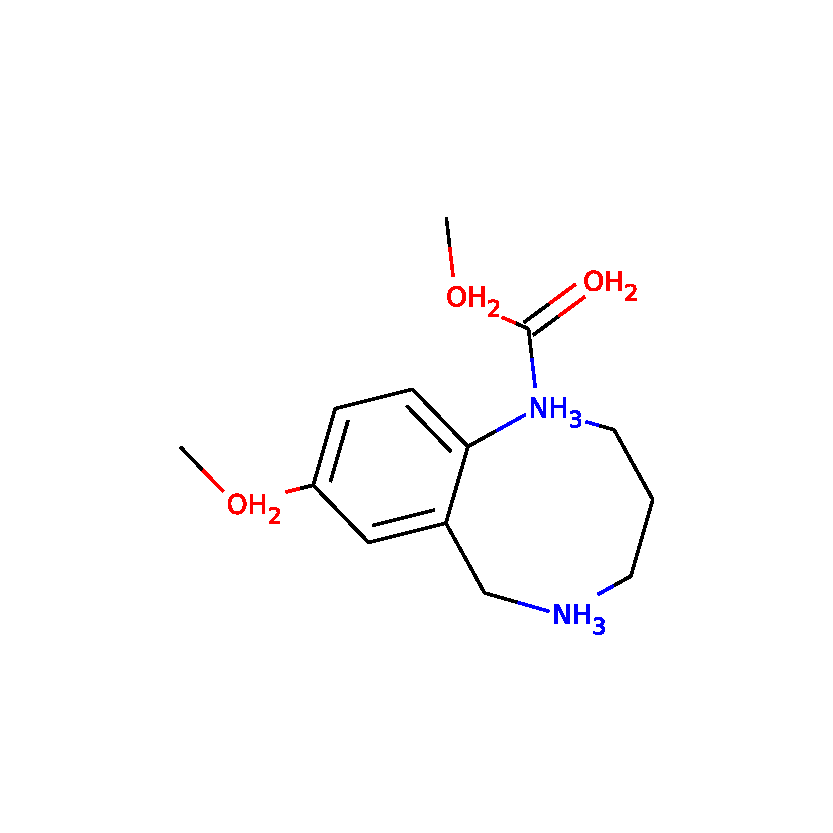
\includegraphics[width=0.22\textwidth]{figures/experiments_figures/molecule_samples/generated_molecule_16_v.pdf} &
        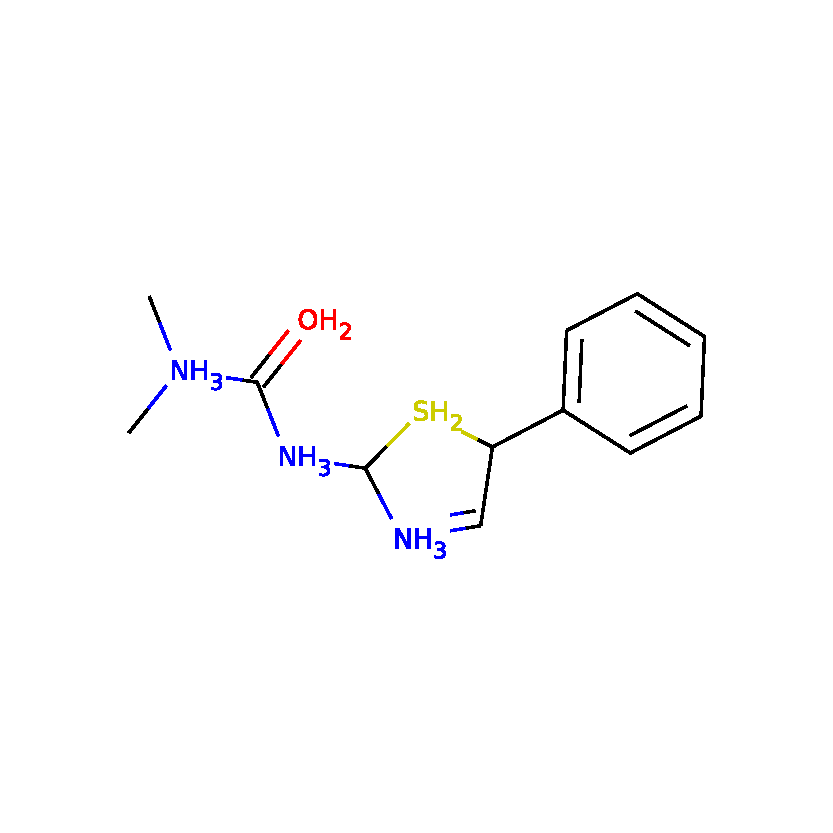
\includegraphics[width=0.22\textwidth]{figures/experiments_figures/molecule_samples/generated_molecule_19_v.pdf} \\
        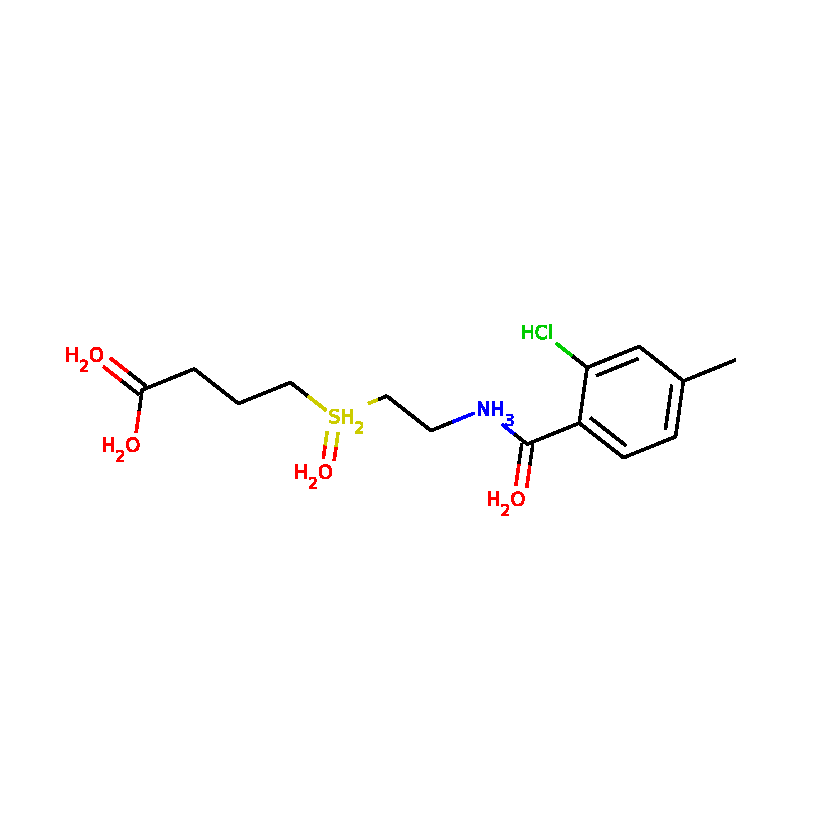
\includegraphics[width=0.22\textwidth]{figures/experiments_figures/molecule_samples/generated_molecule_120_v.pdf} & 
        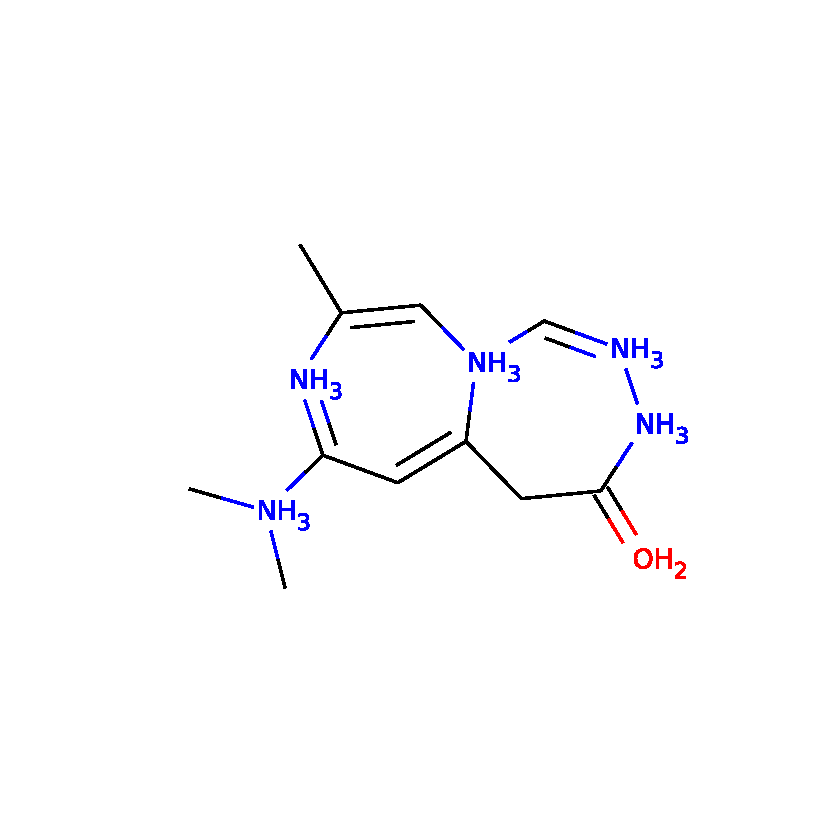
\includegraphics[width=0.22\textwidth]{figures/experiments_figures/molecule_samples/generated_molecule_22_v.pdf} &
        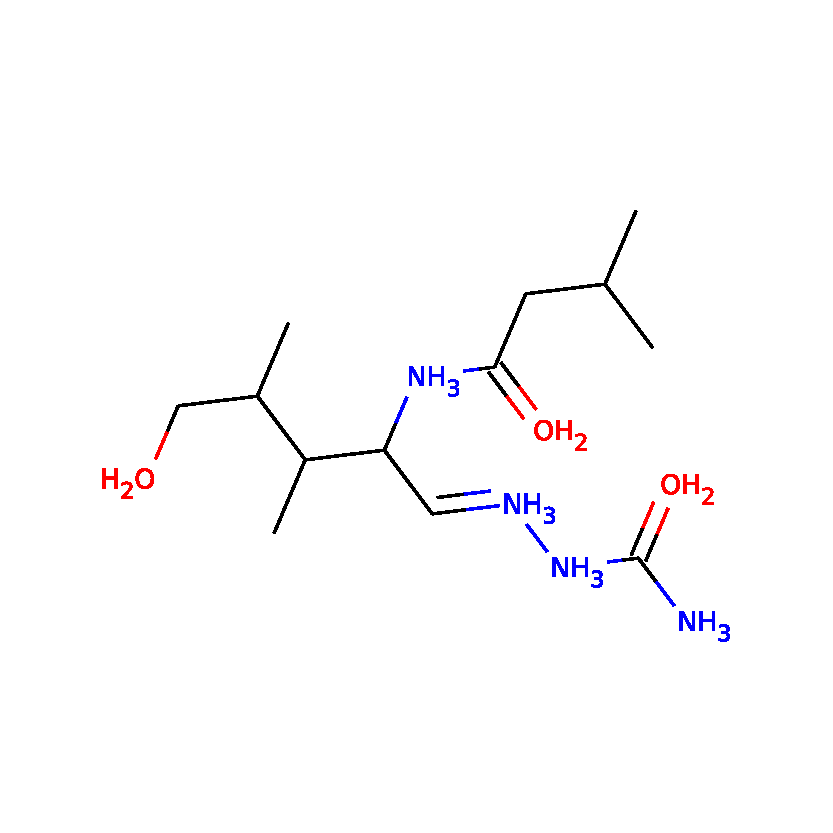
\includegraphics[width=0.22\textwidth]{figures/experiments_figures/molecule_samples/generated_molecule_23_v.pdf} &
        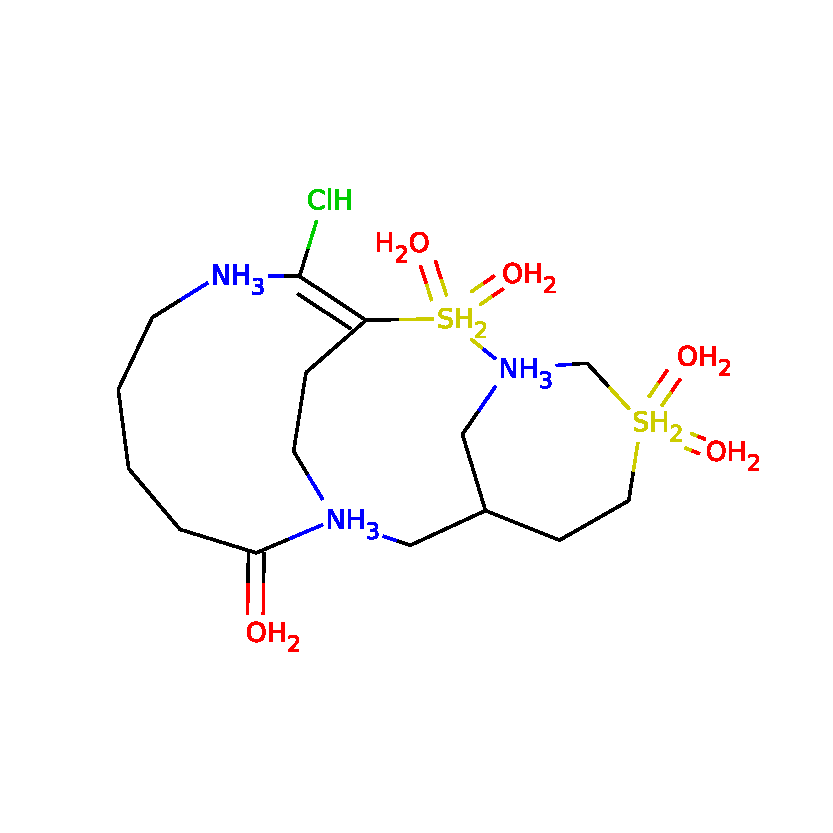
\includegraphics[width=0.22\textwidth]{figures/experiments_figures/molecule_samples/generated_molecule_269_v.pdf}
        \\
    \end{tabular}
    \caption[Samples of molecule graphs from GraphCNF]{Visualization of molecules generated by GraphCNF which has been trained on the Zinc250k \cite{Zinc250k} dataset. Nodes with black connections and no description represent carbon atoms. All of the presented molecules are valid. Best viewed in color and digitally for large molecules.}
    \label{fig:appendix_molecule_generation}
\end{figure}

\subsection{Language modeling}
\label{sec:experiments_language_modeling}

\paragraph{Task} Finally, we test Categorical Normalizing Flows on the task of language modeling. 
The goal of language modeling is to capture grammar and semantic rules of language from large text corpora, and has gained increasingly interest since the recent developments and capabilities of large language models \cite{BERT, GPT2, GPT3}.
Meanwhile, latent-based language models are mostly based on variational autoencoders and suffer in particular from posterior collapse, as decoders like autoregressive models tend to ignore the latent space.
Normalizing flows could potentially offer a new, more stable approach, as they do not rely on strong decoders and work with exact likelihood estimates. 


\paragraph{Datasets} We experiment with two popular character-level datasets, Penn Treebank \cite{PennTreeBank} and text8 \cite{text8}. 
The Penn Treebank consists of 5M characters and has a vocabulary size of $K=51$ characters.
We follow the setup of \citet{SemiDiscreteNFSequence} and split the dataset into sentences of a maximum length of 288. 
Text8 contains about 100M characters and has a vocabulary size of $K=27$. 
We again follow the preprocessing of \citet{mikolov2012subword} and train the models on an input sequence length of 256.
In addition to character-level experiments, we test our model on a word-level language modeling dataset, Wikitext103 \cite{Wikitext}, with a vocabulary size of $K=10,000$. 
Discrete Normalizing Flows are not able to handle such a high number of classes due to its approximations \cite{TranDiscreteFlows}, while Categorical Normalizing Flows can handle such vocabularies. 
Similar to text8, we train the models on a sequence length of 256 for Wikitext103.

\paragraph{Models} For the character-level datasets, we use an encoding dimensionality of 3 per token and increase it to 10 for the word-level experiment.
Each flow applies mixture coupling layers being autoregressive across time and latent dimensions. 
For the character-level experiments, we set the number of mixtures equals to the vocabulary size to verify our motivation on using the mixture coupling layers. 
In the case of the word-level experiment, we limit the number of mixtures to $64$.
We use the same LSTM \cite{LSTM} with hidden size 1024 for all flows and baselines. 

We compare Categorical Normalizing Flows against Latent Normalizing Flows by \citet{SemiDiscreteNFSequence} who reported results on the Penn Treebank dataset.
Their model uses a two-layer Bi-LSTM as encoder and decoder, and 5 flow layers for the prior.
To guarantee a fair comparison and pin down our comparison to the encoding strategy, we also implement a Latent Normalizing Flow with the setup of Categorical Normalizing Flows except the encoding and decoding, for which we use a two-layer Bi-LSTM predicting the mean and scale of logistic distributions.

\begin{table}[t]
	\caption[Results on language modeling]{Results on language modeling measured in bits per character and averaged across 3 seeds (standard deviation shown as $\pm...$). The reconstruction error, also in bits per character, is shown in brackets. Results by \citet{SemiDiscreteNFSequence} did not report a standard deviation.
	}
	\label{tab:result_table_token_level}
	\centering
	\setlength\tabcolsep{4mm}
	\begin{tabular}{lccc}
		\toprule
		\textbf{Model} & \textbf{Penn Treebank} & \textbf{text8} & \textbf{Wikitext103} \\
		\midrule
		LSTM baseline & $1.28$ \footnotesize{$\pm0.01$} & $1.44$ \footnotesize{$\pm0.01$} & $4.81$ \footnotesize{$\pm0.05$}\\[4pt]
		Latent NF & & & \\
		- \citet{SemiDiscreteNFSequence} & $1.42$ \footnotesize{(0.10)} & $-$ & $-$ \\
		- 1 layer & $1.40$ \footnotesize{$\pm0.02$} \footnotesize{(0.04)} & $1.61$ \footnotesize{$\pm0.01$} \footnotesize{(0.03)} & $7.05$ \footnotesize{$\pm0.31$} \footnotesize{(1.09)}\\
		\midrule
		Categorical NF - 1 layer & $1.27$ \footnotesize{$\pm0.01$} \footnotesize{(0.00)} & $1.45$ \footnotesize{$\pm0.01$} \footnotesize{(0.00)} & $5.43$ \footnotesize{$\pm0.09$} \footnotesize{(0.32)}\\
		\bottomrule
	\end{tabular}
\end{table}

\paragraph{Results} The results in Table~\ref{tab:result_table_token_level} show that Categorical Normalizing Flows with a single layer are performing on par with their non-latent autoregressive counterparts. 
The reconstruction loss of the discrete tokens from continuous space, i.e. the average negative log-likelihood of the decoder, is lower than $1e$-$3$bpd showing that the posterior is almost deterministic. 
Furthermore, when comparing to \citet{SemiDiscreteNFSequence}, we see a significant improvement while using only 1 instead of 5 flows and a much simpler encoding.
Our re-implementation 
This underlines the importance of using a factorized posterior and removing any interactions between variables from the decoder. 
One notable difference between our setup of Latent NF and \citet{SemiDiscreteNFSequence} is the lower reconstruction error despite the prior being considerably smaller in number of parameters and depth. 
As the only other major difference is the type of coupling layer (\citet{SemiDiscreteNFSequence} use non-linear squared flows), we can conclude that mixture coupling layers promote the shift of likelihood optimization towards the prior, and push the decoder to being deterministic.

For word-level language modeling, a single mixture coupling layer is not flexible enough to learn all possible sequences.
Thus, we see a small gap between the LSTM baseline and Categorical Normalizing Flows, although the flow's flexibility could be improved by using more transformations/layers.
Nonetheless, this experiment shows that Categorical Normalizing Flows can generalize to large categorical distributions without being limited by gradient approximations or such.
In contrast, Latent Normalizing Flows achieve a considerably worse performance which is also attributed to training difficulties. 
Since decoding $10,000$ categories from a latent space is a challenging task in itself, we experienced instabilities when balancing the reconstruction error of the decoder with the prior likelihood.
These instabilities are also because the decoder, encoder and prior all work on the same latent space but changes in the encoding need to be propagated to the decoder and prior by consecutive gradient updates (i.e. decoder and prior run a step behind the encoder).
Categorical Normalizing Flows, on the other hand, did not show to have those issues as the decoder is independently applied across categorical variables, and therefore much simpler than in Latent Normalizing Flows.

\subsection{Discussion}
\label{sec:experiments_discussion}

The experiments on sets, graphs, and language modeling show that Categorical Normalizing Flows are widely applicable and can model categorical distributions precisely.
In the following section, we will discuss the important aspects of Categorical Normalizing in more detail.
In particular, we take another look at the encoding distributions and elaborate on the reasons why the mixture model is sufficient.
We also visualize the latent space of trained flows to gain further insights into the modeling capability of Categorical Normalizing Flows.
We conclude this section by discussing the differences to Discrete Normalizing Flows under the consideration of the obtained experimental results.

\subsubsection{Encoding distributions} 

Across all the tasks that we experimented on, the simple mixture model encoding has shown to work well with Categorical Normalizing Flows while being the most efficient at the same time.
Despite the additional flexibility, we experienced that the linear flow and variational encoding method mainly relied on a logistic mixture model as well.
This finding might seem counter-intuitive at first as several works have reported a significant gain by applying strong encoding distribution in variational dequantization for the task of image modeling \cite{Flow++, EmielDequantization, VFlow}. 

Besides the natural integration of logistics in our flow architecture which presumably leads to the favoring of a logistic encoding, there are two differences between categorical encoding and dequantization that are potentially crucial for the variational framework. 
Firstly, images are quantized, continuous signals that inherently contain noise from several sources \cite{NoiseModelsImages}. 
This noise can be both independent across pixels (e.g. white noise) or correlated with close-by pixels.
Variational dequantization can model this noise by a flexible dequantization distribution which needs to be complex enough to capture the noise's true mean and variance. 
In categorical distributions, however, we do not have such noise signals as categories are naturally discrete.  

Secondly, in dequantization, the encoding volumes of discrete values have sharp edges, i.e. the probability density function has a sudden change to zero.
As discussed by \citet{Flow++}, such volumes are more challenging to model for a normalizing flow as it requires several additional transformations.
Allowing the flow to change the encoding distribution in the first place simplifies the modeling objective.
Meanwhile, in Categorical Normalizing Flows, we do not have this issue as the volumes per category are separated with regions of low probability density between them, and usually do not contain sharp edges.
Thus, based on these two aspects, we argue that variational encoding does not (significantly) improve the modeling capabilities of Categorical Normalizing Flows, although it is important in the image domain.

The encoding distributions of Categorical Normalizing Flows all rely on the idea of having a factorized decoder across categorical variables.
This not only provides the encoding to be efficient during sampling, but also allows for an exact likelihood estimate in the case of a mixture model or linear encoding.
Latent Normalizing Flows, on the other hand, introduce interactions among variables in the decoder, and thus, models a lower bound. 
In general, we found Latent Normalizing Flows only to work well when we were able to train the decoder to be close to deterministic.
This was the case for the set modeling experiments and the character language modeling, with applying an appropriate loss scheduling, but not for the word-level experiments due to the large number of categories.
Still, in all experiments we experienced Latent NFs to be instable, in particular in the beginning of the training when the decoder propagates high gradients back to the encoder. 
This causes the encoding distribution to change abruptly, and the prior has to adapt to these changes within the next iterations. 
However, this can again lead to a high loss when the transformations in the prior do not fit to the new encoding, and thus map them to points of low likelihood.
Thus, we see a loss peak across couple of iterations until the model balances itself out again, or diverges.
Such situations were encouraged by having rare categories in the dataset, as in the Penn Treebank and Wikitext103.  

Compared to Latent Normalizing Flows, Categorical Normalizing Flows offer two benefits.
Firstly, CNFs are more stable and simpler to train as no loss scheduling is required, and the likelihood remains an exact estimate.
Secondly, the encoding of CNFs is much more efficient than Latent NFs. 
Despite selecting suitable encoder and decoder architectures for the respective tasks, the additional complexity did not show to help in our experiments. 
Thus, we come to the conclusion that Categorical Normalizing Flows are more widely applicable, and Latent NFs might only the better choice if there exists a task-specific decoder that integrates pre-known knowledge about the data.

\subsubsection{Visualization of the latent space} 
\label{sec:experiments_discussion_latent_space}

To gain insights into the inner working of Categorical Normalizing Flows, we visualize the latent space at different stages of the flow.
We hope to see interactions among categories and understand how Categorical Normalizing Flows utilize continuous transformations to learn categorical distributions.
For visualization purposes, we limit the latent space dimensionality to 2 and accumulate the samples across categorical variables. 
We show the mapping of the mixture model to a single logistic by color-coding the modes of each category differently.
The samples in the forward direction are gathered from about 1k categorical data points, each sampled 8 times from the encoding distribution.
For inverting the flow, we sampled 8k times from the base distribution.
For reproducibility, the exact details of the visualization are summarized in Appendix~\ref{sec:appendix_latent_space_visualization}.

\begin{figure}[t!]
    \centering
    \begin{subfigure}{\textwidth}
        \centering
        \begin{tabular}{cccc}
            \textit{Encoding distribution} &
            \textit{Flow layer 4} & 
            \textit{Flow layer 6} & 
            \textit{Base distribution} \\
            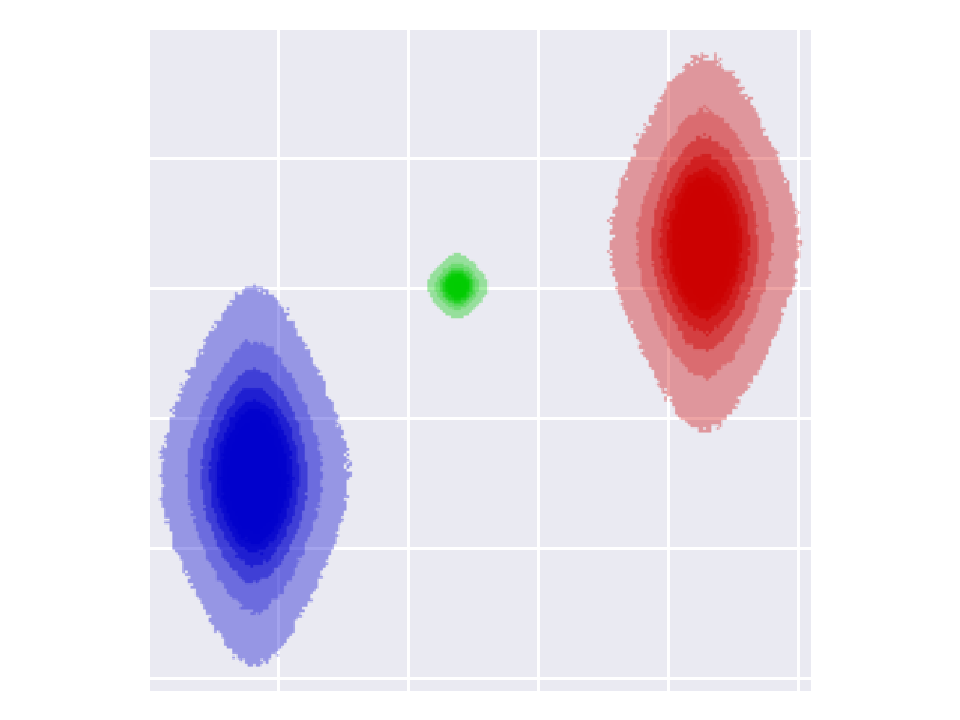
\includegraphics[width=0.225\textwidth]{figures/experiments_figures/latent_space/graph_coloring/layer_forward_01.pdf} & 
            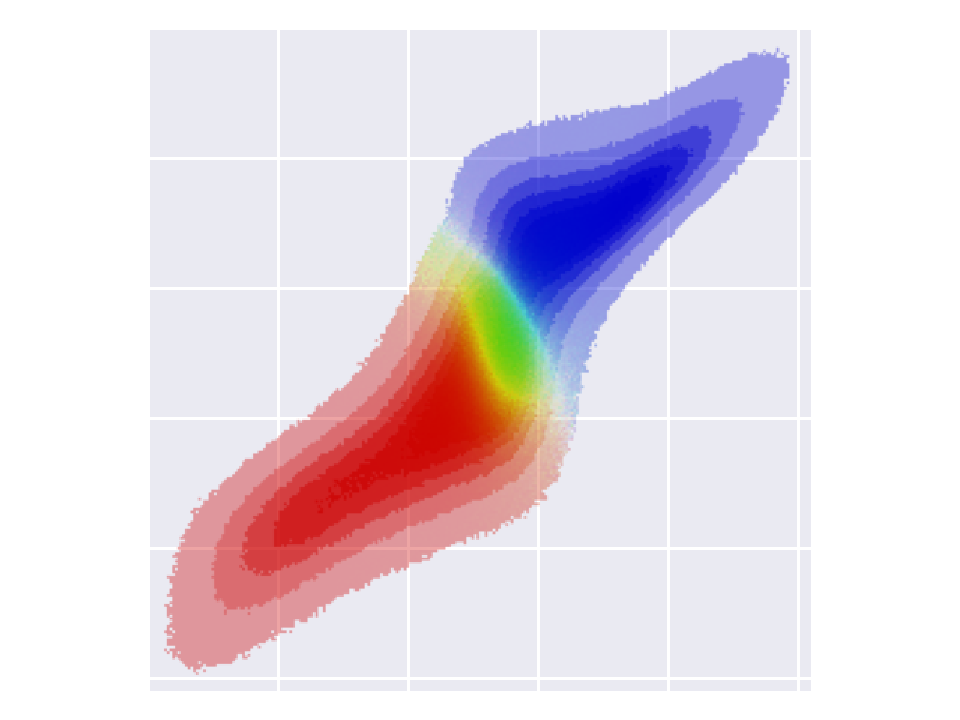
\includegraphics[width=0.225\textwidth]{figures/experiments_figures/latent_space/graph_coloring/layer_forward_13.pdf}  & 
            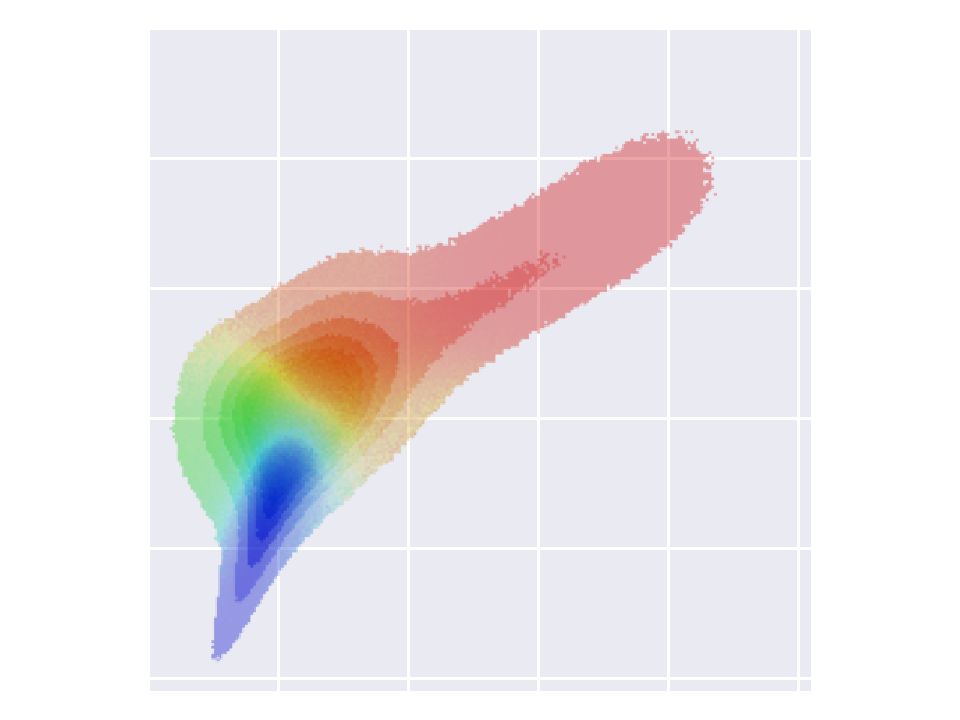
\includegraphics[width=0.225\textwidth]{figures/experiments_figures/latent_space/graph_coloring/layer_forward_19.pdf}  & 
            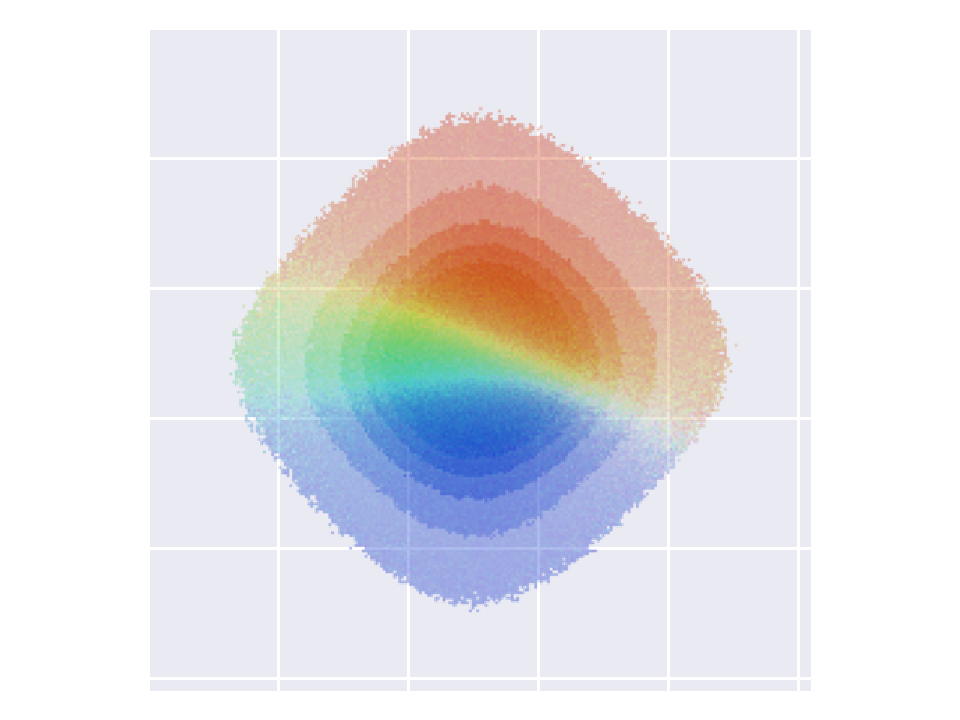
\includegraphics[width=0.225\textwidth]{figures/experiments_figures/latent_space/graph_coloring/layer_forward_25.pdf}
            \\
        \end{tabular}
        \caption{Forward sampling\\[0.5cm] }
    \end{subfigure}
    \begin{subfigure}{\textwidth}
        \centering
        \begin{tabular}{cccc}
            \textit{Encoding distribution} &
            \textit{Flow layer 4} & 
            \textit{Flow layer 6} & 
            \textit{Base distribution} \\
            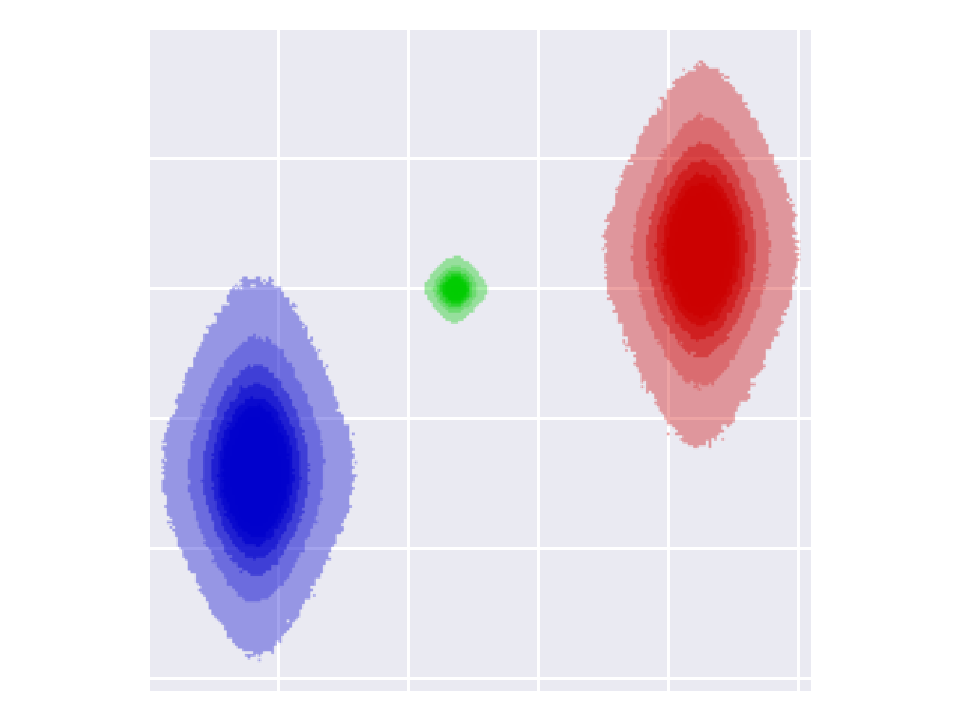
\includegraphics[width=0.225\textwidth]{figures/experiments_figures/latent_space/graph_coloring/layer_reverse_26.pdf} & 
            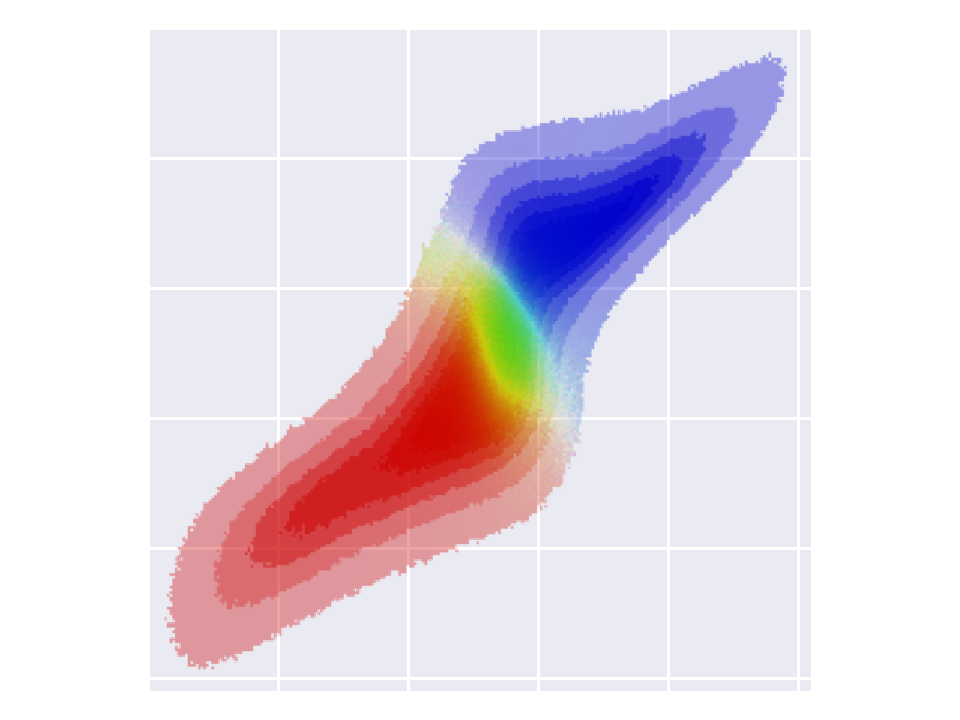
\includegraphics[width=0.225\textwidth]{figures/experiments_figures/latent_space/graph_coloring/layer_reverse_14.pdf}  & 
            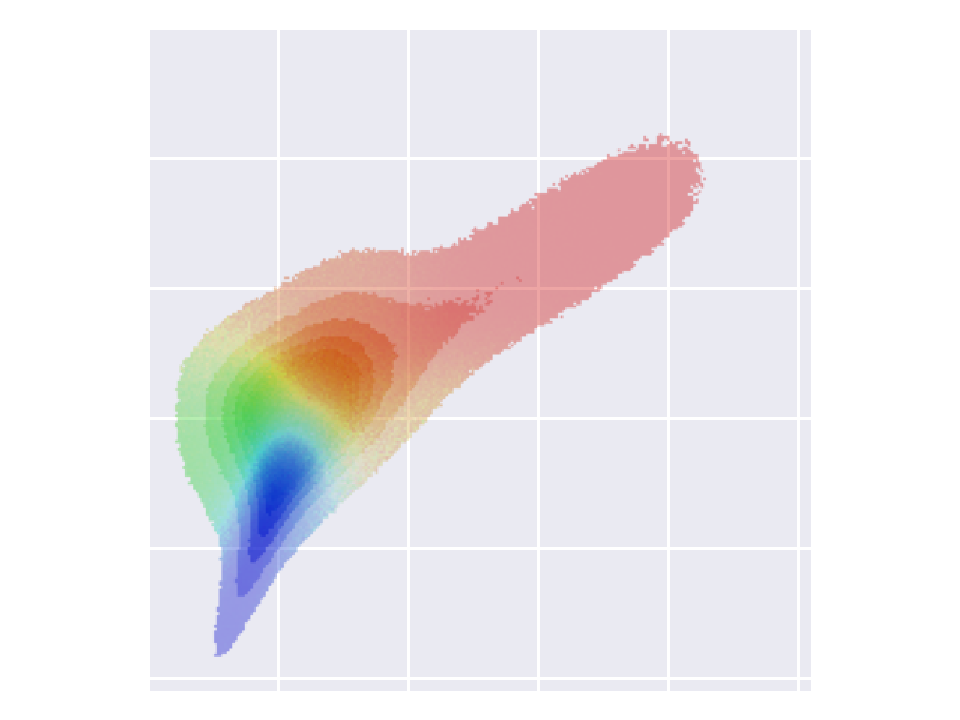
\includegraphics[width=0.225\textwidth]{figures/experiments_figures/latent_space/graph_coloring/layer_reverse_08.pdf}  & 
            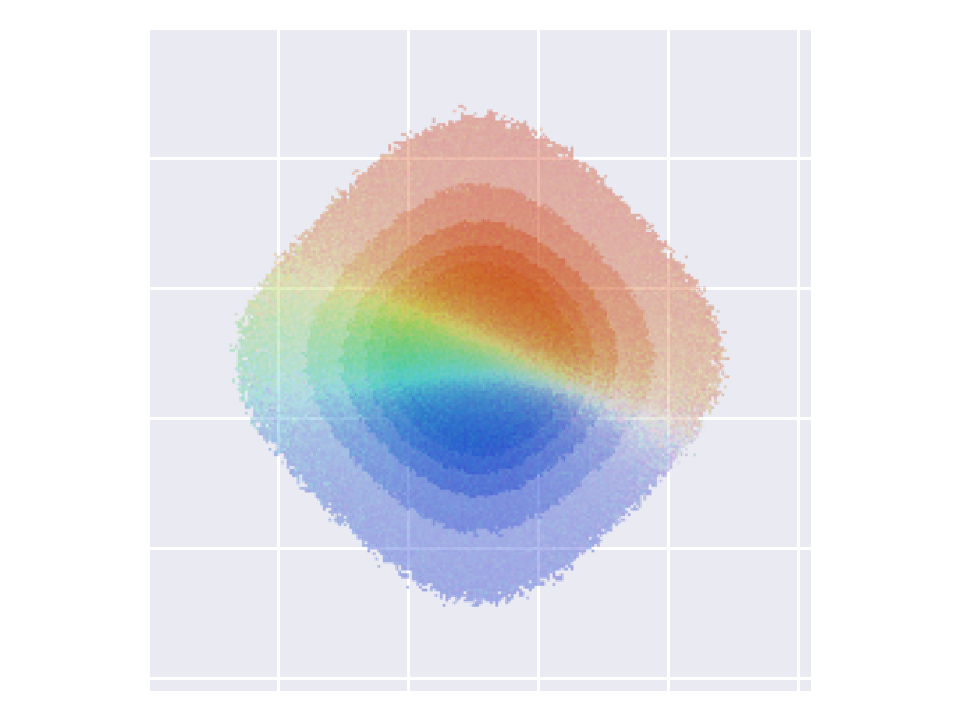
\includegraphics[width=0.225\textwidth]{figures/experiments_figures/latent_space/graph_coloring/layer_reverse_02.pdf}
            \\
        \end{tabular}
        \caption{Reverse sampling\\[0.2cm]}
        \label{fig:experiments_discussion_latent_space_graph_coloring_reverse}
    \end{subfigure}
    \caption[Latent space of graph coloring flow]{Visualization of the latent space in a 8-layer flow trained on graph coloring with 3 categories (shown in red, blue and green; best viewed in color and digital). The density of each category is colored differently and normalized independently. Overlapping distributions are shown by averaging the RGB colors weighted by their probability density. The left most figure shows the learned mixture encoding distribution $q(\bm{z}|\bm{x})$, the center figures show the latent spaces after corresponding coupling flow layers and right most shows the modeled base distribution (logistic). The latent space is scaled to fit into the figure size for each visualization independently. Subfigure (a) shows the probability densities in forward mode, i.e. pushing dataset examples through the flow, and (b) during generation, i.e. when sampling from the base distribution and reversing the flows.
    A larger visualization of all flow layers can be found in Appendix~\ref{sec:appendix_latent_space_visualization}.}
    \label{fig:experiments_discussion_latent_space_graph_coloring}
\end{figure}

Figure~\ref{fig:experiments_discussion_latent_space_graph_coloring} shows the latent space of a GraphCNF model on the task of graph coloring.
The model is trained on the small dataset as a latent dimensionality of 2 has shown to work well there.
The encoding distribution is, as expected, a mixture of three logistic distributions, each with a different mean and scale.
Interestingly, the green color has a significantly smaller scale than the other two, but this pattern is not constant across seeds. 
The layers in between show that the categories are stepwise merged, depending on the specific input/node in a graph.
While in layer 4 we have small areas where multiple categories occur (the yellow, cyan, and purple areas), most parts can be clearly associated with one color.
In layer 6, the combined area is growing and takes on a significant part of the overall probability density.
Finally, the base distribution still seems to be split into three parts, one for each category.
However, when looking closely at the respective parts, we can see that the colors are not pure, meaning that there is also a considerable amount of samples from the other two categories in the parts.
For instance, the red part is \textit{sprinkled} with yellow and purple pixels (the exact location is possibly due to the variance in the visualization).
Hence, we can say that each part resembles a \textit{dominant} color, i.e. if possible the node will be colored respectively, but also supports different colors when necessary.

The latent space that is created when inverting the flows (Figure~\ref{fig:experiments_discussion_latent_space_graph_coloring_reverse}), i.e. during sampling, is almost exactly the same as in the forward direction. 
Minor differences can be spotted in flow layer 6 for the red density for instance, but those do not influence the samples in categorical space. 
Thus, we can validate that the encoding distribution does not constitute any difficulties to the flow and that the flow can accurately model the mixture input distribution.

\begin{figure}[t!]
    \centering
    \begin{subfigure}{\textwidth}
        \centering
        \begin{tabular}{cccc}
            \textit{Encoding distribution} &
            \textit{Flow layer 2} & 
            \textit{Flow layer 3} & 
            \textit{Base distribution} \\
            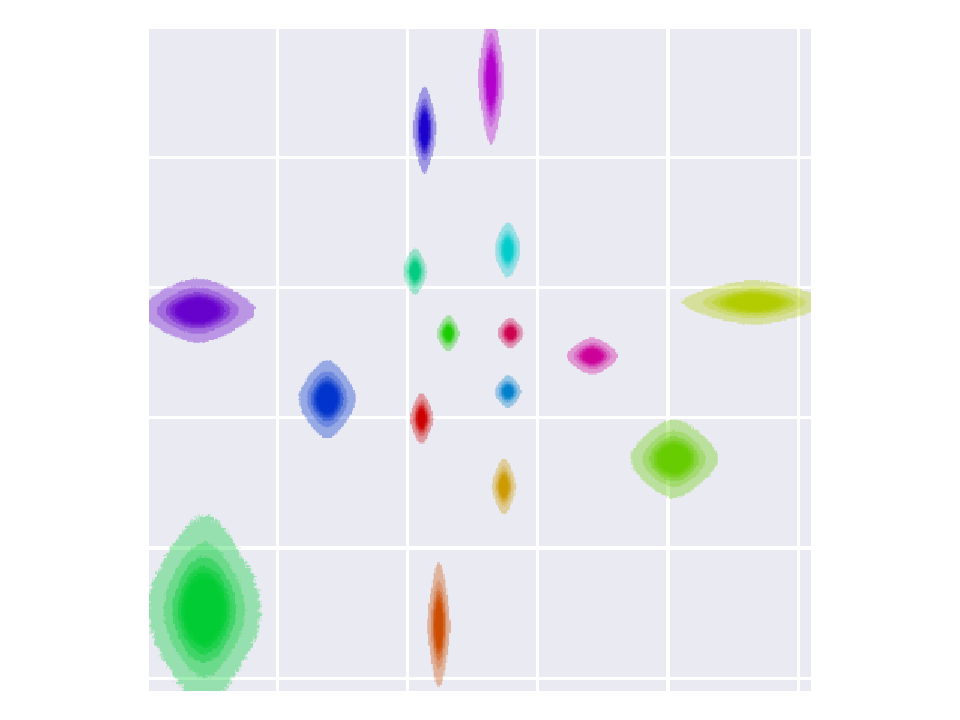
\includegraphics[width=0.225\textwidth]{figures/experiments_figures/latent_space/set_modeling/layer_forward_01.pdf} & 
            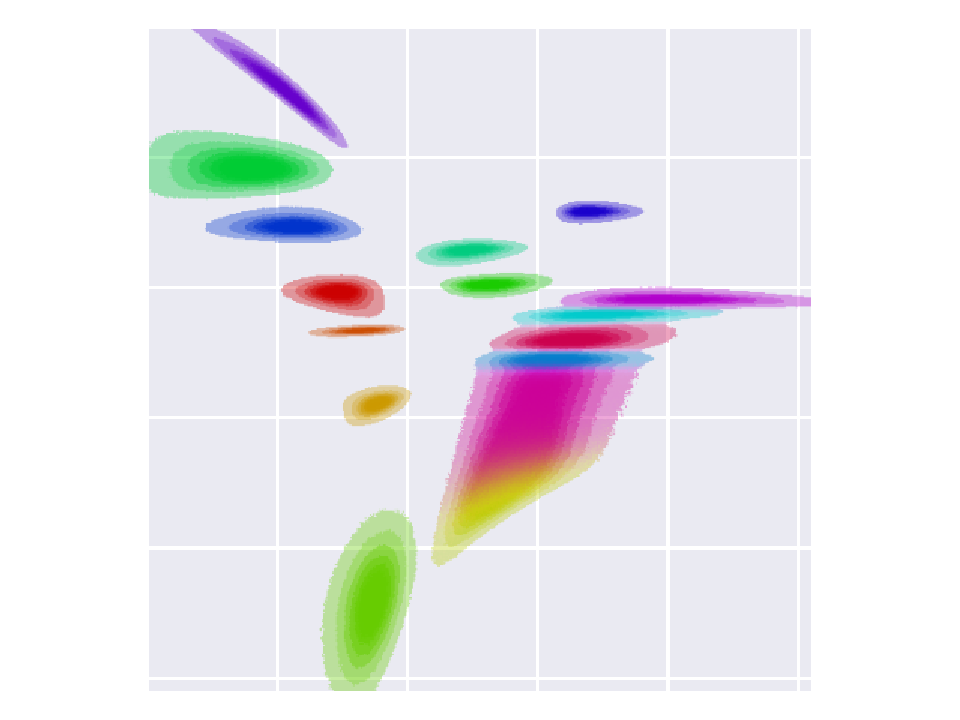
\includegraphics[width=0.225\textwidth]{figures/experiments_figures/latent_space/set_modeling/layer_forward_07.pdf}  & 
            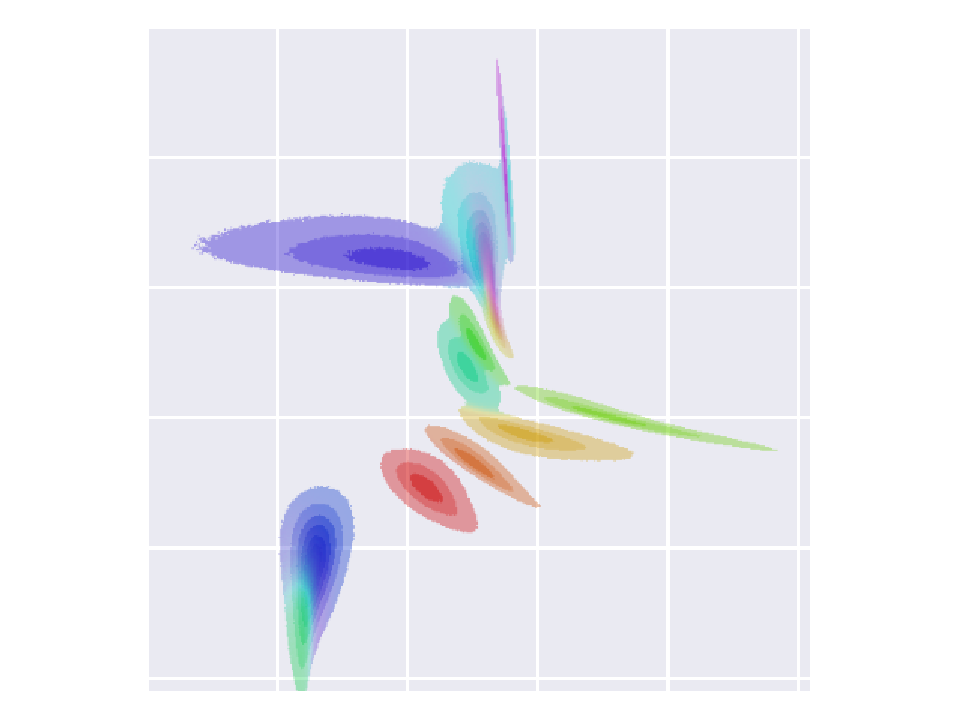
\includegraphics[width=0.225\textwidth]{figures/experiments_figures/latent_space/set_modeling/layer_forward_10.pdf}  & 
            \includegraphics[width=0.225\textwidth]{figures/experiments_figures/latent_space/set_modeling/layer_forward_13.pdf}
            \\
            \multicolumn{4}{c}{\includegraphics[width=0.95\textwidth]{figures/experiments_figures/latent_space/set_modeling/legend_visu.pdf}}\\
        \end{tabular}
        \caption{Forward sampling\\[0.5cm] }
    \end{subfigure}
    \begin{subfigure}{\textwidth}
        \centering
        \begin{tabular}{cccc}
            \textit{Encoding distribution} &
            \textit{Flow layer 2} & 
            \textit{Flow layer 3} & 
            \textit{Base distribution} \\
            \includegraphics[width=0.225\textwidth]{figures/experiments_figures/latent_space/set_modeling/layer_reverse_13.pdf} & 
            \includegraphics[width=0.225\textwidth]{figures/experiments_figures/latent_space/set_modeling/layer_reverse_07.pdf}  & 
            \includegraphics[width=0.225\textwidth]{figures/experiments_figures/latent_space/set_modeling/layer_reverse_04.pdf}  & 
            \includegraphics[width=0.225\textwidth]{figures/experiments_figures/latent_space/set_modeling/layer_reverse_01.pdf}
            \\
            \multicolumn{4}{c}{\includegraphics[width=0.95\textwidth]{figures/experiments_figures/latent_space/set_modeling/legend_visu.pdf}}\\
        \end{tabular}
        \caption{Reverse sampling\\[0.2cm]}
    \end{subfigure}
    \caption[Latent space of set modeling flow]{Visualization of the latent space in a 4-layer flow trained on set modeling with 16 categories (best viewed in color and digital).
    The illustration follows the same setup as Figure~\ref{fig:experiments_discussion_latent_space_graph_coloring}.
    The legend beneath the latent space visualization show the color assignment for the 16 categories $C_{0}$ to $C_{15}$.}
    \label{fig:experiments_discussion_latent_space_set}
\end{figure}

To show the effect of more categories, we also visualize the latent space of a Categorical Normalizing Flow trained on set modeling in Figure~\ref{fig:experiments_discussion_latent_space_set}. 
We can see that some categories are combined at different stages throughout the flow. 
As there are no clear relations among the categories, the decision of which categories to combine when is arbitrary and changes across seeds.
Similarly to the base distribution in graph coloring, we experience a clear separation of categories in the logistics.
Again, those colors are not pure and any category can be created based on any of sample in the logistic.
Note that the visually larger purple part is due to the combination of categories with similar colors ($C_{10}, C_{11}, C_{12}$, and $C_{13}$) and not because of a larger probability density of a single category.

In conclusion, the visualization of the latent space shows that:
\begin{itemize}
    \item The transformation flexibility provided by the continuous space is used to partly merge densities of different categories. For instance in graph coloring, the probability density of green and red are merged in the first flows for those nodes that can have any of the two colors without breaking the validity constraint (for example, see Figure~\ref{fig:experiments_graph_coloring_examples}a, bottom right node). 
    Meanwhile, other variables stay with a unique category.
    This merge process happens throughout the flow at different stages, until all categories have been merged into the base distribution.
    \item The continuous base distribution is split into areas of dominant colors. Such a separation can help to influence the categorical output during sampling, for instance when we are looking for a certain output. 
    This can be particularly of interest for applications like drug discovery and property optimization which work on latent generative models.
    \item Looking at the latent space allows us to interpret the model. With a sufficient number of samples, the probability density per category can be visualized throughout the flow and shows how the model maps the mixture model back to the base distribution. Furthermore, the merging process shows the interactions among categories that are modeled by the flow.
\end{itemize}

\subsubsection{Comparison to Discrete Normalizing Flows}

One of the key aspects of Categorical Normalizing Flows' expressiveness is the flexible transformations in continuous space. 
As seen in the last subsection, the flow often combines parts of probability densities of two or more categories while other parts stay separated.
Such transformations seem to be crucial for modeling categorical distributions.
In contrast, Discrete Normalizing Flows do not allow such transformation.
Due to the invertibility constrain in discrete space, categories can only be permuted or combined by an equal ratio (i.e. two categories can be mapped to the same output by a coupling layer if the input contains the information which category it is). 
Stochastic combinations or ones with flexible weights would break the invertibility because instead of probability densities, categories are represented by a single number. 
This limits Discrete Normalizing Flows in becoming universal (i.e. being able to learn any input distribution) as continuous normalizing flows are.

Nevertheless, representing categories by a single number has one decisive advantage: the input is always the same for a discrete data point.
When training Categorical Normalizing Flows, the first step is to sample from the encoding distribution $\tilde{\bm{z}}\sim q(\bm{z}|\bm{x})$, which will be different every time we sample.
To learn the true categorical distribution, the flow has to model an (optimal) transformation for each continuous data point. 
This variation in the input increases computation and time needed for training considerably.
For instance, when we compare the training speed of the LSTM baseline with the autoregressive Categorical Normalizing Flow on language modeling (text8 dataset), the flow takes almost 5 times as many iterations to obtain the same performance as the baseline.
Similarly, on simple datasets like set shuffling, a considerable amount of optimization steps are necessary to achieve the close-to-optimal performance (about 100k iterations) although there is little variation in the categorical dataset. 
The phenomenon of long training times for continuous normalizing flows has also been found on image modeling \cite{VFlow, Flow++}.

Therefore, a future direction would be to combine the benefits of a discrete input with the flexible transformations of Categorical Normalizing Flows.
One possibility to do so is to introduce stochastic layers into the normalizing flows \cite{StochasticNF, SurVAE}.
While this breaks the initial invertibility assumption of normalizing flows, it uses variational inference with a similar idea as the encoding distribution of Categorical Normalizing Flows. 
Especially the idea of surjective flows by \citet{SurVAE}, where only the forward direction of a flow layer is deterministically invertible while the reverse is stochastic, can be an interesting direction for Discrete NFs.
However, it should be kept in mind that Discrete Normalizing Flows have also the disadvantage of differentiating through discrete operators which introduce additional, considerable challenges.
Thus, we leave this idea as a potential starting point for future work.
% IDEA: We can express an autoregressive model as surjective discrete NF

% \begin{itemize}
%     \item Discuss in more detail the variational encoding (paragraph conclusion)
%     \item Visualize the latent space and its transitions (check graph coloring and set modeling)
%     \item GraphCNF (permutation invariance)
%     \begin{itemize}
%         \item GraphCNF is more memory intensive and requires more parameters. RNNs on the other hand are slow in sampling. If sampling is not a major priority and an "optimal" order is known, RNN might work well. In other cases and more general, GraphCNF is the better choice.
%     \end{itemize}
%     \item General continuous normalizing flows
%     \begin{itemize}
%         \item One current limitation of continuous flows is the training speed. While purely autoregressive models can learn simple categorical distributions within a few iterations, normalizing flows take much longer. Even if NFs are autoregressive.
%         We found that this noise can be helpful and acts as a regularizer for small datasets as it has been the case for the Penn Treebank in the language experiments. 
%         On the other hand, this sampling noise is not there anymore in Discrete Normalizing Flows. 
%         Possible future direction: combine flexibility of Categorical NF with "discreteness" of Discrete NFs 
%     \end{itemize}
%     \item 
% \end{itemize}
\newpage
\section{Conclusion}
\label{sec:conclusion}
We present Categorical Normalizing Flows which learn a categorical, discrete distribution by a continuous normalizing flow.
This is implemented by a joint objective to optimize the representation of categorical data in continuous latent space via variational inference, and the model likelihood of a normalizing flow on this space. 
We thereby use variational inference only for representing the discrete data in continuous space, while all interactions between categorical variables should be learned in the normalizing flow.
Hence, we enforce a factorized (approximate) posterior which maintains almost unique decoding while still allowing flexible encoding distributions. 
In experiments on sets, graphs, and language modeling, we find that a plain mixture model is sufficient for modeling discrete distributions accurately while providing an efficient way for encoding and decoding categorical data. 
In addition, we experience that the optimal encoding dimensionality of the continuous latent space does not only depend on the number of categories, but also on the complexity of the interactions among variables.

Based on Categorical Normalizing Flows, we propose a normalizing flow on graph modeling, GraphCNF.
In contrast to autoregressive models, GraphCNF is permutation-invariant to the order of nodes in a graph, meaning it assigns an equal likelihood to any permutation.
Furthermore, we introduce a three-step generation process that adds the nodes, edge attributes, and adjacency matrix stepwise to the latent space to improve efficiency and stabilize training.
Tested on the tasks of graph coloring and molecule generation, GraphCNF outperforms autoregressive and other one-shot approaches constituting a new state-of-the-art for normalizing flows on molecule generation. 

These results emphasize the potential of normalizing flows on modeling categorical distributions, especially for such with non-sequential data. 
The domains and applications we experimented on in this thesis are not exhaustive and Categorical Normalizing Flows can be applied to many more. 
One application with increasing interest is parallel language modeling which could enable deep models like GPT3 \cite{GPT3} with a much greater generation speed.
Furthermore, recent work by \citet{VFlow} has shown that combining dequantization with a variational framework for increasing the number of dimensions leads to considerable improvements in image modeling, which agrees with our findings on categorical data.

Besides, the insights we gained in how Categorical Normalizing Flows model discrete distributions can potentially help to improve the design of Discrete Normalizing Flows.
While continuous approaches have smooth gradients but inherit noise during training, discrete flows have to tackle optimization issues and their limited modeling capability.
Combining continuous approaches with discrete can be a promising direction as in such models flows can choose between the best of both worlds, depending on the modeling task at hand.
\newpage

\renewcommand\refname{Bibliography}
\addcontentsline{toc}{section}{Bibliography}
\bibliographystyle{bibstyle}
\bibliography{references_mendeley}

\newpage
\addtocontents{toc}{\protect\setcounter{tocdepth}{1}} 
\appendix
\titleformat{\section}[hang]
{\Large\bfseries}
{\thesection.}{0.4em}{}
\titlespacing{\section}{0pc}{0.5cm}{0.5cm}
\titleformat{\subsection}[hang]
{\large\bfseries}
{\thesubsection.}{0.4em}{}
\titlespacing{\subsection}{0pc}{0.4cm}{0.3cm}


\section{Expressiveness of logistic mixture coupling layers}
\label{sec:appendix_mixture_optimality}

The following section details the proof to show that under mild assumptions, Categorical Normalizing Flows with autoregressive logistic mixture coupling layers can be as powerful as other non-latent based recurrent neural networks with a pure autoregressive likelihood objective. 
This has not been the case for previous attempts on modeling categorical data with normalizing flows in continuous space as seen in \cite{SemiDiscreteNFSequence}.

We start with a single layer autoregressive mixture coupling layer and assume that the categories are encoded by a mixture of logistics. 
The base distribution is also a standard logistic.
Recall that the logistic mixture coupling for a single element $z$ is defined by the following transformation:
\begin{equation}
    y = \sigma^{-1}\left(\sum_{i=1}^{K} \pi_i \sigma\left(\frac{z-\mu_i}{\exp(-s_i)}\right)\right)\cdot \exp(a)+b
\end{equation}
where $\bm{\pi}, \bm{\mu}, \bm{\sigma}, a$ and $b$ are parameterized by a neural network, and $K$ is the number of mixtures.
As we are aiming to model a standard logistic as base distribution, we set $a=0,b=0$.
The log-determinant Jacobian (LDJ) of a mixture coupling layer for a single element is then as follows:
\begin{eqnarray}
\gamma_i & = & \frac{z-\mu_i}{\exp(-s_i)}\\
\text{LDJ}_{\text{coup}} & = & \log \left(\sum \pi_i \cdot \exp\left[\gamma_i - s_i - 2\log\left(1+\exp(\gamma_i)\right)\right]\right)\\
& = & \log \left(\sum \pi_i \cdot \exp\left[\gamma_i - s_i\right]/\left(1+\exp(\gamma_i)\right)^2\right)
\end{eqnarray}
The coupling layer maps a mixture of $K$ logistics back to a single one.
Hence, in this case, the optimal setting is if those $K$ mixtures represent the logistics for the categories in the encoding distribution.
Additionally, the variational framework ensures that we train the encoding mixtures to be clearly separated. 
Thus, we can assume that for a sampled latent $z$ from $q(z|x)$, $|\gamma_j|\gg0$ for all $j\in\{1,...,K\}$ except one, which we denote here with $i$. Then we can reduce the LDJ to:
\begin{eqnarray}
\text{LDJ}_{\text{coup}} & = & \log \pi_i + \gamma_i - s_i - 2\log\left(1+\exp(\gamma_i)\right)\\
& = & \log \pi_i + \log\left(\exp(\gamma_i)/\left(1+\exp(\gamma_i)\right)\right) - s_i - \log\left(1+\exp(\gamma_i)\right)\\
& = & \log \pi_i - s_i - \log\left(1+\exp(-\gamma_i)\right) - \log\left(1+\exp(\gamma_i)\right)
\end{eqnarray}	
Next, we have to add the LDJ we obtain from the encoding distribution. 
For a single element $z$, this is:
\begin{eqnarray}
\text{LDJ}_{\text{encode}} & = & s_i + \log\left(1+\exp(-\gamma_i)\right) + \log\left(1+\exp(\gamma_i)\right)
\end{eqnarray}
where we reuse the index $i$ from $\text{LDJ}_{\text{coup}}$. 
The overall objective we are left with for an input $x$ is:
\begin{eqnarray}
\text{LDJ}_{\text{model}} & = & \text{LDJ}_{\text{encode}} + \text{LDJ}_{\text{coup}} \\
& = & \log \pi_i
\end{eqnarray}	
Therefore, optimizing the logistic mixture coupling layer reduces to optimizing a softmax distribution over categories which is exactly the same objective as a standard autoregressive model on categorical distribution. 
We have shown that this property also holds in practice as can be seen at the experiments on language modeling (Section~\ref{sec:experiments_language_modeling}).

\newpage
\section{Visualization of the latent space}
\label{sec:appendix_latent_space_visualization}

In the following, we outline the visualization method of the latent space used in Section~\ref{sec:experiments_discussion_latent_space}.


\begin{figure}[b!]
    \centering
    \begin{tabular}{ccc}
        \textit{Encoding distribution} &
        \textit{Flow layer 1} & 
        \textit{Flow layer 2} \\
        \includegraphics[width=0.3\textwidth]{figures/experiments_figures/latent_space/graph_coloring/layer_forward_01.pdf} & 
        \includegraphics[width=0.3\textwidth]{figures/experiments_figures/latent_space/graph_coloring/layer_forward_04.pdf}  & 
        \includegraphics[width=0.3\textwidth]{figures/experiments_figures/latent_space/graph_coloring/layer_forward_07.pdf}
        \\[0.4cm]
        \textit{Flow layer 3} &
        \textit{Flow layer 4} & 
        \textit{Flow layer 5} \\
        \includegraphics[width=0.3\textwidth]{figures/experiments_figures/latent_space/graph_coloring/layer_forward_10.pdf} & 
        \includegraphics[width=0.3\textwidth]{figures/experiments_figures/latent_space/graph_coloring/layer_forward_13.pdf}  & 
        \includegraphics[width=0.3\textwidth]{figures/experiments_figures/latent_space/graph_coloring/layer_forward_16.pdf}
        \\[0.4cm]
        \textit{Flow layer 6} &
        \textit{Flow layer 7} & 
        \textit{Base distribution} \\
        \includegraphics[width=0.3\textwidth]{figures/experiments_figures/latent_space/graph_coloring/layer_forward_19.pdf} & 
        \includegraphics[width=0.3\textwidth]{figures/experiments_figures/latent_space/graph_coloring/layer_forward_22.pdf}  & 
        \includegraphics[width=0.3\textwidth]{figures/experiments_figures/latent_space/graph_coloring/layer_forward_25.pdf}
        \\
    \end{tabular}
    \caption[Complete latent space of graph coloring flow (large)]{Visualization of the latent space for all 8 layers of the flow applied on graph coloring (see Figure~\ref{fig:experiments_discussion_latent_space_graph_coloring} for an explanation of the figure). We only show the forward direction as the reverse only differs in negligible aspects.}
    \label{fig:appendix_latent_space_visualization_graph_coloring}
\end{figure}

The first step we take is to collect about 8,000 examples from the training set and forward them through the model as we have done it during training.
Thereby, we save the latent representation $\bm{z}$ after each flow block consisting of an activation normalization, invertible 1x1 convolutions, and a logistic mixture coupling layer.
To reduce the variance, we repeat this process 32 times, each time with different samples from the encoding distribution $q(\bm{z}|\bm{x})$.
After collecting all samples, we convert the observed latents per layer into a histogram in the continuous space with 512 bins for each dimension.
Additionally, we accumulate the histograms across categorical variables to obtain a more stable and general impression of the probability densities in latent space.

To show the densities per category, we color the bins depending on the proportion of latents that represent a specific category. 
For instance, for graph coloring, we visualize the three categories with blue, green, and red. 
If at a position multiple categories occur, we average their RGB color based on the proportion of latents assigned to each category.
In order to see the latent space of all categories equally, we normalize the probability density per category independently.
This means that we first create a histogram for each category separately, then normalize it to have a maximum of 1, and finally combine the histogram of all categories.
Although this strategy does not represent densities across categories correctly, we are able to visualize the densities per category accurately and have no issues with strongly peaked distribution.
If we would have normalized the joint histogram, for instance, the blue and red densities in the encoding distribution (Figure~\ref{fig:appendix_latent_space_visualization_graph_coloring}) would not have been visible.

Finally, we also bin the histogram values to get a clearer distinction between dense and sparse probability mass.
Areas with lower density are more transparent than other parts in the figure and appear with a lighter color.
This gives us finally latent space visualization shown in Figure~\ref{fig:experiments_discussion_latent_space_graph_coloring}, \ref{fig:experiments_discussion_latent_space_set} and \ref{fig:appendix_latent_space_visualization_graph_coloring}.

% \begin{figure}[b!]
%     \centering
%     \begin{tabular}{ccc}
%         \textit{Encoding distribution} &
%         \textit{Flow layer 1} & 
%         \textit{Flow layer 2} \\
%         \includegraphics[width=0.3\textwidth]{figures/experiments_figures/latent_space/set_modeling/layer_forward_01.pdf} & 
%         \includegraphics[width=0.3\textwidth]{figures/experiments_figures/latent_space/set_modeling/layer_forward_04.pdf} & 
%         \includegraphics[width=0.3\textwidth]{figures/experiments_figures/latent_space/set_modeling/layer_forward_07.pdf}
%         \\[0.4cm]
%         \textit{Flow layer 3} &
%         \textit{Base distribution} & \\
%         \includegraphics[width=0.3\textwidth]{figures/experiments_figures/latent_space/set_modeling/layer_forward_10.pdf} & 
%         \includegraphics[width=0.3\textwidth]{figures/experiments_figures/latent_space/set_modeling/layer_forward_13.pdf} & 
%         \\
%     \end{tabular}
%     \caption[Complete latent space of graph coloring flow (large)]{Visualization of the latent space for all 8 layers of the flow applied on graph coloring (see Figure~\ref{fig:experiments_discussion_latent_space_graph_coloring} for an explanation of the figure). We only show the forward direction as the reverse only differs in negligible aspects.}
%     \label{fig:appendix_latent_space_visualization_graph_coloring}
% \end{figure}

\newpage
\section{Experimental settings}
\label{sec:appendix_hyperparams}

In this section, we detail the hyperparameter settings and datasets for all experiments. All experiments have been implemented using the deep learning framework PyTorch \cite{PyTorch}.
The experiments for graph coloring and molecule generation have been executed on a single NVIDIA TitanRTX GPU. The average training time was between 1 and 2 days. The set and language experiments have been executed on a single NVIDIA GTX1080Ti in 4 to 16 hours. All experiments have been repeated with at least 3 different random seeds. Our code is published at \href{https://github.com/phlippe/CategoricalNF}{https://github.com/phlippe/CategoricalNF}.

\subsection{Set modeling}
\label{sec:appendix_hyperparams_set}
\paragraph{Dataset details} We use two toy datasets, set shuffling and set summation, to simulate a discrete distribution over sets in our experiments. Note that we do not have a classical split of train/val/test dataset, but instead train and test the models on samples from the same discrete distribution. This is because we want to verify whether a categorical normalizing flow and other baselines can model an arbitrary discrete distribution. 
The special property of sets is that permuting the elements of a set still represent the same set. However, a generative model still has to learn all possible permutations. While an autoregressive model considers those permutations as different data points, a permutation-invariant model as Categorical Normalizing Flow contains an inductive bias to assign the exact same likelihood to any permutation. 

In set shuffling, we only have one set to model which is the following (with categories $C_{1}$ to $C_{16}$):
$$\{C_{1}, C_{2}, C_{3}, C_{4}, C_{5}, C_{6}, C_{7}, C_{8}, C_{9}, C_{10}, C_{11}, C_{12}, C_{13}, C_{14}, C_{15}, C_{16}\}$$
This set has $16!$ possible permutations and therefore challenging to model. The optimal likelihood in bits per element is calculated by $\log_2 \left(16!\right) / 16 \approx 2.77$. %where $16^{16}$ represents all possible assignments for an arbitrary set of 16 elements with 16 possible values. 

The dataset set summing contains of 2200 valid sets for $N=16$ and $L=42$. An example for a valid set is:
$$\{1, 1, 1, 1, 2, 2, 2, 2, 2, 2, 3, 3, 3, 3, 6, 8\}$$
For readability, the set is sorted by ascending values, although any permutation of the elements represent the exact same set. Taking into account all possible permutations of the sets in the dataset, we obtain a optimal likelihood of $\log_2 \left(6.3\cdot10^{10}\right) / 16 \approx 2.24$.
The values for the sequence length $N$ and sum $L$ was chosen such that the task is challenging enough to show the differences between Categorical Normalizing Flows and its baselines, but also not too challenging to prevent unnecessarily long training times and model complexities.

\paragraph{Hyperparameter details} Table~\ref{tab:appendix_hyperparameters_sets} shows an overview of the hyperparameters per model applied on set modeling. We use the notation ``\{val1, val2, ...\}'' to show the different values we have tried during the hyperparameter search. Thereby, the underlined value denotes the hyperparameter value with the best performance and finally was being used to generate the results in Table~\ref{tab:result_table_sets}. 

The number of encoding coupling layers in Categorical Normalizing Flows are sorted by the used encoding distribution. The mixture model uses no additional coupling layers, while for the linear flows, we apply 4 affine coupling layers using an external input for the discrete category. For the variational encoding distribution $q(\bm{z}|\bm{x})$, we use 4 mixture coupling layers across the all latent variables $\bm{z}$ with external input for $\bm{x}$. A larger dimensionality of the latent space per element showed to be beneficial for all encoding distributions. Note that due to a dimensionality larger than 1 per element, we are able to apply the channel mask instead of a chess mask and maintain permutation invariance compared to the baselines.

In variational dequantization and Discrete NF, we sort the categories randomly for set shuffling (the distribution is invariant to the category order/assignment) and in ascending order for set summation. In Discrete NF, we followed the published code from \citet{TranDiscreteFlows} for their coupling layers and implemented it in PyTorch \cite{PyTorch}. We use a discrete prior over the set elements which is jointly optimized with the flow. However, we experienced significant optimization issues due to the straight-through gradient estimator in the Gumbel Softmax. 

Across this paper, we experiment with the two optimizers Adam \cite{Adam} and RAdam \cite{RAdam}, and experienced RAdam to work slightly better. The learning rate decay is applied at every update and leads to exponential decay. However, we did not observe the choice of this hyperparameter to be crucial.

\begin{table}[ht!]
    \centering
    \caption[Hyperparameter overview for the set modeling experiments]{Hyperparameter overview for the set modeling experiments presented in Table~\ref{tab:result_table_sets}}
    \label{tab:appendix_hyperparameters_sets}
    \renewcommand{\arraystretch}{1.2}
    \begin{tabular}{lccc}
        \toprule
        \textbf{Hyperparameters} & \textbf{Categorical NF} & \textbf{Var. dequant.} & \textbf{Discrete NF}\\
        \midrule
        Latent dimension & \{2, \underline{4}, 6\} & 1 & 16\\
        \#Encoding couplings & - / 4 / 4 & 4 & - \\
        \#Coupling layers & 8 & 8 & \{4, \underline{8}\} \\
        Coupling network & Transformer & Transformer & Transformer \\
        - Number of layers & 2 & 2 & 2 \\
        - Hidden size & 256 & 256 & 256 \\
        Mask & Channel mask & Chess mask & Chess mask\\
        \#Mixtures & 8 & 8 & - \\
        Batch size & 1024 & 1024 & 1024\\
        Training iterations & 100k & 100k & 100k\\
        Optimizer & \{Adam, \underline{RAdam}\} & RAdam & \{SGD, \underline{Adam}, RAdam\}\\
        Learning rate & 7.5e-4 & 7.5e-4 & \{1e-3, \underline{1e-4}, 1e-5\} \\
        Learning rate decay & 0.999975 & 0.999975 & 0.999975\\
        Temperature (GS) & - & - &  \{\underline{0.1}, 0.2, 0.5\}\\
        \bottomrule
    \end{tabular}
\end{table}

\subsection{Graph coloring}
\label{sec:appendix_hyperparams_graph_coloring}

\paragraph{Dataset details}
In our experiments, we focus on the 3-color problem meaning that a graph has to be color with using $K=3$ colors. We generate the datasets by randomly sampling a graph and using an SAT solver\footnote{We have used the following solver from the OR-Tools library in python: \href{https://developers.google.com/optimization/cp/cp_solver}{https://developers.google.com/optimization/cp/cp\_solver}} for finding one valid coloring assignment. 
In case no solution can be found, we discard the graph and sample a new graph. 
We further ensure that every graph cannot be colored by less than 3 colors in order to exclude too simple graphs. 
For creating the graphs, we take inspiration from \citet{GraphColoringDL} and first uniformly sample the number of nodes between $10\leq|V|\leq20$ for the small dataset, and $25\leq|V|\leq50$ for the large dataset.
Next, we sample a value $p$ between $0.1$ and $0.3$ which represents the probability of having an edge between a random pair of nodes. Thus, $p$ controls how dense a graph is, and we aim to have both dense and sparse graphs in our dataset. 
For each pair of nodes, we sample from a Bernoulli distribution with probability $p$ of adding an edge between the two nodes or not. Finally, we check whether each node has at least one connection and that all nodes can be reached from any other node. This ensures that we have one connected graph and not multiple sub-graphs. 
Overall, we create a train/val/test size of 192k/24k/24k for the small dataset, and 450k/20k/30k for the large graphs. 

During training, we randomly permute the colors of a graph (e.g. red becomes blue, blue becomes green, green becomes red) as any permutation is a valid color assignment. When we sample a color assignment from our models, we explicitly use a temperature value of 1.0. For the autoregressive model and the VAE, this means that we sample from the softmax output. A common alternative is to take the argmax, which corresponds to a temperature value of 0.0. However, we stick to the original distribution because we want to test whether the models capture the full discrete distribution of valid color assignments and not only the most likely solution. For the normalizing flow, a temperature of 1.0 corresponds to sampling from the prior distribution as it was used during training.

\paragraph{Hyperparameter details} Table~\ref{tab:appendix_hyperparameters_graph_coloring} shows an overview of the used hyperparameters. If ``/'' is used in the table, the first parameter refers to the hyperparameter value used on a small dataset and the second for the larger dataset. The activation function used within the graph neural networks is GELU \cite{GELU}. Interestingly we experience that a larger latent space dimensionality is crucial for larger graphs despite having the same number of categories as the small dataset. This shows that having an encoding being flexible in the number of dimensions can be further important for datasets where complex relations between categorical variables need to be modeled. Increasing the number of dimensions on the small dataset did not show any significant differences in performance. 
The number of mixtures in the mixture coupling layers is in general beneficial to be large. However, this can also increase the sampling time. In the case of sampling time being crucial, the number of mixtures can be decreased in the cost of slightly worse performance.

The input to the autoregressive model is the graph with the color assignment at time step $T$ where each category including unassigned nodes is represented by an embedding vector. We experiment with an increasing number of hidden layers. While more layers are especially important for sub-optimal node ordering, the performance does not significantly improve for more than 5 layers. As the sampling time also increases linearly with the number of layers, we use 5 hidden layers for the models.

For the variational autoencoder, we encode each node by a latent vector of size 4. As VAEs have shown to benefit from slowly adding the KL divergence between prior and posterior to the loss, we experiment with a scheduler where the slope is based on a sigmoid and stretched over 10k iterations. 

\begin{table}[ht!]
    \centering
    \caption[Hyperparameter overview for the graph coloring experiments]{Hyperparameter overview for graph coloring experiments presented in Table~\ref{tab:result_table_graph_coloring}}
    \label{tab:appendix_hyperparameters_graph_coloring}
    \renewcommand{\arraystretch}{1.2}
    \begin{tabular}{lccc}
        \toprule
        \textbf{Hyperparameters} & \textbf{GraphCNF} & \textbf{Variational AE} & \textbf{Autoregressive}\\
        \midrule
        Latent dimension & \{\underline{2}, 4\} / \{2, 4, \underline{6}, 8\} & 4 & -\\
        \#Coupling layers & \{6, \underline{8}\} & - & - \\
        (Coupling) network & GAT & GAT & GAT \\
        - Number of layers & \{3, \underline{4}, 5\} & 5 & \{3, 4, \underline{5}, 6, 7\} \\
        - Hidden size & 384 & 384 & 384 \\
        - Number of heads & 4 & 4 & 4 \\
        Mask & Channel mask & - & -\\
        \#Mixtures & \{4, \underline{8}, 16\} / \{4, 8, \underline{16}\} & - & - \\
        Batch size & 384 / 128 & 384 / 128 & 384 / 128\\
        Training iterations & 200k & 200k & 100k\\
        Optimizer & RAdam & RAdam & RAdam \\
        Learning rate & 7.5e-4 & 7.5e-4 & 7.5e-4 \\
        KL scheduler & - & \{1.0, \underline{0.1$\to$0.5}, 0.1$\to$1.0\} & - \\
        \bottomrule
    \end{tabular}
\end{table}

\paragraph{Detailed results}
Table~\ref{tab:appendix_results_graph_coloring} shows the standard deviation of the results reported in Table~\ref{tab:result_table_graph_coloring}. 
Each model was run with 3 different seeds.

\begin{table}[t]
	\caption[Detailed results on graph coloring]{Results on the graph coloring problem, including standard deviation over 3 seeds. The column \textit{time} is excluded since it is constant over seeds.}
	\label{tab:appendix_results_graph_coloring}
	\centering
	\begin{tabular*}{\columnwidth}{@{\extracolsep{\fill}}l*{4}{c}}
		\toprule
		& \multicolumn{2}{c}{$10\leq|V|\leq20$} & \multicolumn{2}{c}{$25\leq|V|\leq50$} \\
		\cmidrule{2-3} \cmidrule{4-5}
		\textbf{Method} & \textbf{Validity} & \textbf{Bits per node} & \textbf{Validity} & \textbf{Bits per node}  \\
		\midrule
		VAE & $44.95\%$ \footnotesize{$\pm 5.32\%$} & $0.84$ \footnotesize{$\pm 0.04$} & $7.75\%$ \footnotesize{$\pm 1.59\%$} & $0.64$ \footnotesize{$\pm 0.02$} \\
		RNN$+$Smallest\_first & $76.86\%$ \footnotesize{$\pm 0.84\%$} & $0.73$ \footnotesize{$\pm 0.02$} & $32.27\%$ \footnotesize{$\pm 1.41\%$} & $0.50$ \footnotesize{$\pm 0.01$}\\
		RNN$+$Random & $88.62\%$ \footnotesize{$\pm 0.65\%$} & $0.70$ \footnotesize{$\pm 0.01$} & $49.28\%$ \footnotesize{$\pm 1.53\%$} & $0.46$ \footnotesize{$\pm 0.01$}\\
		RNN$+$Largest\_first & $93.41\%$ \footnotesize{$\pm 0.42\%$} & $0.68$ \footnotesize{$\pm 0.01$} & $\bm{71.32\%}$ \footnotesize{$\pm 0.77\%$} & $\bm{0.43}$ \footnotesize{$\pm 0.01$}\\
		\midrule
		GraphCNF & $\bm{94.56\%}$ \footnotesize{$\pm 0.55\%$} & $\bm{0.67}$ \footnotesize{$\pm 0.00$} & $66.80\%$ \footnotesize{$\pm 1.14\%$} & $0.45$ \footnotesize{$\pm 0.01$}\\
		$-$ Affine & $93.90\%$ \footnotesize{$\pm 0.68\%$} & $0.69$ \footnotesize{$\pm 0.02$} & $65.78\%$ \footnotesize{$\pm 1.03\%$} & $0.47$ \footnotesize{$\pm 0.01$}\\
		\bottomrule
	\end{tabular*}
\end{table}


\subsection{Molecule generation}

\paragraph{Dataset details} The Zinc250k \cite{Zinc250k} dataset we use contains 239k molecules of which we use 214k molecules for training, 8k for validation and 17k for testing. We follow the preprocessing of \citet{GraphAF} and represent molecules in the kekulized form in which hydrogen is removed. This leaves the molecules with up to 38 heavy atoms, with a mean and median size of about 23.  The smallest graph consists of 8 nodes. Thereby, Zinc250k considers molecules with 8 different atom types where the distribution is significantly imbalanced. The most common atom is carbon with 73\% of all nodes in the dataset. Besides oxygen (10\%) and nitrogen (12\%), the rest of the atoms occur in less than 2\% of all nodes, with the rarest atom being Bromine (0.002\%). Between those atoms, the dataset contains 3 different bonds or edge types, namely a single, double and triple covalent bonds describing how many electrons are shared among the atoms. In over 90\% of all node pairs there exist no bond. In 7\% of the cases, the atoms are connected with a single connection, 2.4\% with a double and 0.02\% with a triple connection. A similar imbalance is present in the Moses dataset and is based on the properties of molecules. Figure~\ref{fig:appendix_molecule_generation_dataset_statistics} visualizes the dataset statistics for both Zinc250k and Moses. Nevertheless, we experienced that GraphCNF was able to generate a similar distribution, where adding the third stage (adding virtual edges later) considerably helped to stabilize the edge imbalance. 



\paragraph{Hyperparameter details} We summarize our hyperparameters in Table~\ref{tab:appendix_hyperparameters_molecule_generation}. Generally, a higher latent dimensionality is beneficial for representing nodes/atoms, similar to the graph coloring task. However, we experienced that a lower dimensionality for edges is slightly better, presumably because the flow already has a significant amount of latent variables for edges. Many edges, especially the virtual ones, do not contain much information.
In addition, a deeper flow showed to gain better results offering more complex transformations. However, in contrast to the graph coloring model, GraphCNF on molecule generation requires a considerable amount of memory as we have to model a feature vector per edge. Nevertheless, we did not experience any issues due to the limited batch size of 96, and during testing, we could scale up the batch size easily to more than 128 on an NVIDIA GTX 1080Ti for both datasets. 


\begin{table}[ht!]
    \centering
    \caption[Hyperparameter overview for the molecule generation experiments]{Hyperparameter overview for molecule generation experiments presented in Table~\ref{tab:result_table_molecule_generation_zinc250k} and \ref{tab:result_table_molecule_generation_moses}}
    \label{tab:appendix_hyperparameters_molecule_generation}
    \renewcommand{\arraystretch}{1.2}
    \begin{tabular}{lc}
        \toprule
        \textbf{Hyperparameters} & \textbf{GraphCNF}\\
        \midrule
        Latent dimension (V/E) & \{4, \underline{6}, 8\} / \{\underline{2}, 3, 4\}\\
        \#Coupling layers ($f_1$/$f_2$/$f_3$) & 4 / \{4, \underline{6}\} / \{4, \underline{6}\} \\
        Coupling network ($f_1$/$f_{2,3}$) & Relational GCN / Edge-GNN\\
        - Number of layers ($f_1$/$f_2$/$f_3$) & \{3/3/3, \underline{3/4/4}, 4/4/4\}\\
        - Hidden size (V/E) & \{\underline{256}, 384\} / \{\underline{128}, 192\} \\
        Mask & Channel mask\\
        \#Mixtures (V/E) & \{8, \underline{16}\} / \{4, \underline{8}, 16\}\\
        Batch size (Zinc250k/Moses) & 64 / 96\\
        Training iterations & 150k\\
        Optimizer & RAdam \cite{RAdam}\\
        Learning rate & {2e-4, \underline{5e-4}, 7.5e-4, 1e-3}\\
        \bottomrule
    \end{tabular}
\end{table}

\begin{figure}
    \centering
    \begin{subfigure}{0.49\textwidth}
       \centering
       \includegraphics[width=\linewidth]{figures/experiments_figures/dataset_figures/zinc250k/zinc250k_node_distribution.pdf}
       \caption{Zinc250k: Node distribution}
    \end{subfigure}
    \hfill
    \begin{subfigure}{0.49\textwidth}
       \centering
       \includegraphics[width=\linewidth]{figures/experiments_figures/dataset_figures/moses/moses_node_distribution.pdf}
       \caption{Moses: Node distribution}
    \end{subfigure}
    \begin{subfigure}{0.49\textwidth}
       \centering
       \includegraphics[width=\linewidth]{figures/experiments_figures/dataset_figures/zinc250k/zinc250k_node_attributes.pdf}
       \caption{Zinc250k: Node attributes}
    \end{subfigure}
    \hfill
    \begin{subfigure}{0.49\textwidth}
       \centering
       \includegraphics[width=\linewidth]{figures/experiments_figures/dataset_figures/moses/moses_node_attributes.pdf}
       \caption{Moses: Node attributes}
    \end{subfigure}
    \begin{subfigure}{0.49\textwidth}
       \centering
       \includegraphics[width=\linewidth]{figures/experiments_figures/dataset_figures/zinc250k/zinc250k_edge_attributes.pdf}
       \caption{Zinc250k: Edge attributes}
    \end{subfigure}
    \hfill
    \begin{subfigure}{0.49\textwidth}
       \centering
       \includegraphics[width=\linewidth]{figures/experiments_figures/dataset_figures/moses/moses_edge_attributes.pdf}
       \caption{Moses: Edge attributes}
    \end{subfigure}
    \caption[Dataset statistic of Zinc250k and Moses]{Dataset statistic of Zinc250k and Moses. (a,b) The node count distribution represents the number of nodes per graph in the dataset. (c,d) The plot shows the frequency of an arbitrary node having a specific categorical node attribute, i.e. atom type. (e,f) Similar to the node attributes, we visualize here the percentage of edges being single, double or triple bonds. The category "virtual" represent the cases where there is no connection/bond between two atoms. }
    \label{fig:appendix_molecule_generation_dataset_statistics}
\end{figure}
\newpage


\subsection{Language modeling}

\paragraph{Dataset details} The three datasets we use for language modeling are the Penn Treebank \cite{PennTreeBank}, text8 \cite{text8} and Wikitext103 \cite{Wikitext}. The Penn Treebank with a preprocessing of \citet{mikolov2012subword} consists of approximately 5M characters and has a vocabulary size of $K=51$. We follow the setup of \citet{SemiDiscreteNFSequence} and split the dataset into sentences of a maximum length of 288. Furthermore, instead of an end-of-sentence token, the length is passed to the model and encoded by an external discrete prior which is created based on the sentence lengths in the training dataset.

Text8 contains about 100M characters and has a vocabulary size of $K=27$. We again follow the preprocessing of \citet{mikolov2012subword} and split the dataset into 90M characters for training, and 5M characters each for validation and testing. We train and test the models on a sequence length of 256.

In contrast to the previous two datasets, we use Wikitext103 as a word-level language dataset. First, we create a vocabulary and limit it to the most frequent 10,000 words in the training corpus. We thereby use pre-trained Glove \cite{Glove} embeddings to represent the words in the baseline LSTM networks and to determine the logistic mixture parameters in the encoding distribution of Categorical Normalizing Flows. Due to this calculation of the mixture parameters, we use a small linear network as a decoder. The linear network consists of three linear layers of hidden size 512 with GELU \cite{GELU} activation and output size of 10,000 (the vocabulary size). Similarly to text8, we train and test the models on an input sequence length of 256.

\paragraph{Hyperparameter details} The hyperparameters for the language modeling experiments are summarized in Table~\ref{tab:appendix_hyperparameters_language_modeling}. We apply the same hyperparameters for the flow and baseline if applicable. The best latent dimensionality for character-level has been shown to be 3, although larger dimensionality showed to gain similar performance. For the word-level dataset, it is beneficial to increase the latent dimensionality to 10. However, note that 10 is still significantly smaller than the Glove vector size of 300. As Penn Treebank has a limited training dataset on which LSTM networks easily overfit, we use a dropout \cite{Dropout} of 0.3 throughout the models and dropout an input token with a chance of 0.1. The other datasets seemed to benefit slightly by a small input dropout to prevent overfitting at later stages of the training.

\begin{table}[ht!]
    \centering
    \caption[Hyperparameter overview for the language modeling experiments]{Hyperparameter overview for the language modeling experiments presented in Table~\ref{tab:result_table_token_level}}
    \label{tab:appendix_hyperparameters_language_modeling}
    \renewcommand{\arraystretch}{1.2}
    \begin{tabular}{lccc}
        \toprule
        \textbf{Hyperparameters} & \textbf{Penn Treebank} & \textbf{text8} & \textbf{Wikitext103}\\
        \midrule
        (Max) Sequence length & 288 & 256 & 256 \\
        Latent dimension & \{2, \underline{3}, 4\} & \{2, \underline{3}, 4\} & \{8, \underline{10}, 12\}\\
        \#Coupling layers & 1 & 1 & 1 \\
        Coupling network & LSTM & LSTM & LSTM \\
        - Number of layers & 1 & 2 & 2 \\
        - Hidden size & 1024 & 1024 & 1024 \\
        - Dropout & \{0.0, \underline{0.3}\} & 0.0 & 0.0 \\
        - Input dropout & \{0.0, 0.05, \underline{0.1}, 0.2\} & \{0.0, \underline{0.05}, 0.1\} & \{0.0, \underline{0.05}, 0.1\} \\
        \#Mixtures & 51 & 27 & 64 \\
        Batch size & 128 & 128 & 128\\
        Training iterations & 100k & 150k & 150k\\
        Optimizer & RAdam & RAdam & RAdam\\
        Learning rate & 7.5e-4 & 7.5e-4 & 7.5e-4 \\
        \bottomrule
    \end{tabular}
\end{table}

% \newpage
% \input{sections/notes.tex}

\end{document}
